% Version of Document Management
% $Revision: $

% Version with Table of Contents generation, to create pdf version

% pour l'ajout ci-dessous, voir https://tex.stackexchange.com/questions/720126/compiling-of-pdf-a-1b-compatible-document-fails-due-to-latex-error-loading-a-cl
\RequirePackage[2024-05-01]{latexrelease}

\title{Manuel Utilisateur de CodeBlocks}
\def\newcharencode{utf8}        % set character encoding
\ProvidesFile{booleans.tex}[2006/11/01 HighTec template]
\RequirePackage{snapshot}       % list dependencies in .dep
\RequirePackage{ifthen}         % control structures
\makeatletter
\@ifundefined{newcharencode}{   % cp1252
    \RequirePackage[ansinew]{inputenc}% package for input encoding under windows
}{
    %\RequirePackage{ucs}       % utf-8
    \RequirePackage[utf8]{inputenc}
}
\newboolean{html}               % specials for presentation with beamer.cls
\newboolean{book}               % print document as book
\newboolean{mathmode}           % specials for propser presentation
\newboolean{tabreg}             % for generation of list of tables otherwise set Tabreg false
\newboolean{figreg}             % for generation of list of figures otherwise set Figreg false
\newboolean{glossreg}           % for generation of glossary
\newboolean{acroreg}            % for generation of acronyms
\newboolean{nomreg}             % for generation of nomenclature
\newboolean{urlreg}             % for generation of url catalogue
\newboolean{bibreg}             % for generation of Bibliography otherwise set Bibreg false
\newboolean{multiidx}           % for generation of multiple index
\newboolean{changereg}          % list of changes
\newboolean{indreg}             % for generation of Index otherwise set Indreg false
\newboolean{shortdocu}          % use for short docu
%% set defaults %%%%%%%%%%%%%%%%%%%%%%%%%%%%%%%%%%%
\setboolean{html}{false}        % for option for common_pack.tex
\setboolean{book}{false}        % print document as book
\setboolean{mathmode}{false}    % enable amslatex
\setboolean{tabreg}{false}      % for generation of list of tables otherwise set Tabreg false
\setboolean{figreg}{false}      % for generation of list of figures otherwise set Figreg false
\setboolean{glossreg}{false}    % for generation of glossary
\setboolean{acroreg}{false}     % for generation of acronyms
\setboolean{nomreg}{false}      % for generation of nomenclature
\setboolean{urlreg}{false}      % for generation of url catalogue
\setboolean{bibreg}{false}      % for generation of Bibliography otherwise set Bibreg false
\setboolean{multiidx}{false}    % for generation of multiple index
\setboolean{changereg}{false}   % list of changes
\setboolean{indreg}{false}      % for generation of Index otherwise set Indreg false
\setboolean{shortdocu}{false}   % use for short docu
       % boolean declaration
% booleans already defined and set in mystyles/booleans, eventually set to an other value here ...
\setboolean{urlreg}{true}       % for url catalogue
\setboolean{bibreg}{false}      % for bibliography
\setboolean{indreg}{false}      % for index generation
\setboolean{shortdocu}{true}    % oneside document
%\setboolean{figreg}{true}       % for figure list
%\setboolean{tabreg}{true}       % for table list
%\setboolean{html}{true}

%\def\lngfr{french}
%\def\lngen{english}
%\def\lngge{german}

%%%%% options %%%%%%%%%
\def\lang{french}
\def\graphmode{final}           % graphmodes: draft: box; final: including figures

% generate url catalog for toolchain
\def\urlfilename{mystyles/url_codeblocks}

%%%%%%%% parameter for titlepage %%%%%%%%%%
\def\Subject{Code::Blocks}
\def\Title{Manuel Utilisateur}
\def\DocVersion{2.1.17}

% style for documentation
\ProvidesFile{format_docu.tex}[2007/05/26 HighTec template]
%%%%%%%%%%%%%%%%%%%%%%%%%%%%%%%%%%%%%%%%%%%%%%%%%%%%%%%%%%%%%%%%%%%%%%%%%%%%%%%%%%%%%%%%%%%%%%%%%%%%%%%%%%%%%%%%%%%%%%%%%%%%%%%
% Some of the ifthenelse (but apparently/strangely not All) have problems when they are used by MikTeX 22.10 though it was OK 
% with a previous version 22.03, particularly when they are used to build an html version by htlatex.
% They have been replaced by the standard TeX syntax \if ...[ \else ... ]\fi in different .tex files within mystyles folder.
%%%%%%%%%%%%%%%%%%%%%%%%%%%%%%%%%%%%%%%%%%%%%%%%%%%%%%%%%%%%%%%%%%%%%%%%%%%%%%%%%%%%%%%%%%%%%%%%%%%%%%%%%%%%%%%%%%%%%%%%%%%%%%%
\ifthenelse{\boolean{shortdocu}}{\def\docupagemode{oneside}}{\def\docupagemode{twoside}}
%\ifthenelse{\boolean{shortdocu}}{\def\docupagemode{twoside=false}}{\def\docupagemode{twoside=true}}
\ifthenelse{\equal{\lang}{german}}{%
    % german language
    \documentclass[index=totoc,ngerman,12pt,\docupagemode,paper=a4,headings=normal,headsepline,numbers=noenddot,footsepline,\graphmode]{scrbook}
%    \documentclass[idxtotoc,ngerman,12pt,\docupagemode,a4paper,normalheadings,headsepline,pointlessnumbers,footsepline,\graphmode]{scrbook}
}{
    \ifthenelse{\equal{\lang}{french}}{%
    % french language
        \documentclass[index=totoc,french,12pt,\docupagemode,paper=a4,headings=normal,headsepline,numbers=noenddot,footsepline,\graphmode]{scrbook}
    }{
    % english by default
        \documentclass[index=totoc,english,12pt,\docupagemode,paper=a4,headings=normal,headsepline,numbers=noenddot,footsepline,\graphmode]{scrbook}
    }
}

\ifthenelse{\boolean{nomreg}}{\usepackage[\lang]{nomencl}\makeglossary}{}
\ifthenelse{\boolean{glossreg}}{\usepackage{glosstex}}{}

% common packages
\ProvidesFile{common_pack.tex}[2005/01/02 HighTec template]
\makeatletter
\@ifundefined{htmlmode}{\usepackage{mparhack}}{}% correct marginal in document
\makeatother
% select conditional text within document
\usepackage{version}
\def\includecomment{\includeversion}
\def\excludecomment{\excludeversion}

\ifthenelse{\equal{\lang}{german}}{%
    \usepackage[ngerman]{babel}                 % translate figure -> Abbildung etc.
    \usepackage{ngerman}                        % new sgerman hyphenation
}{}

%\ifthenelse{\equal{\lang}{french}}{%
%    \usepackage[french]{babel}                 % Should be nice, but give errors ! At least with listings package
%    \usepackage{french}
%}{}
% produce several index
\ifthenelse{\boolean{indreg}}%
{%
    \ifthenelse{\boolean{multiidx}}{\usepackage[makeindex]{splitidx}}{\usepackage[makeindex]{splitidx}}
    \newindex[Index]{idx}                       % common index
}{}
\usepackage{fancyvrb, listings}                 % verbatim input and complex verbatim
\usepackage{url}                                % breaking urls
\usepackage{float, morefloats}                  % utility for placing figures with here [H] option; subfigure placing% normally # of floats 18 -> with more float 38
\usepackage{afterpage}                          % figures not before first reference
\afterpage{\clearpage}                          %
\ifthenelse{\boolean{mathmode}}{\usepackage{amsbsy,amsmath,amstext,amsfonts,amssymb}}{}% for AMS-Latex -> formula
\usepackage{xcolor}                             % switch from color to xcolor package (driver independent)
\usepackage{ifpdf}                              % with this package \ifpdf \else \fi
\ifpdf                                          % We are not running pdftex
    \usepackage[pdftex, \graphmode]{graphicx}   % Package for graphics import
    \usepackage{epstopdf}                       % pdflatex understands eps -> use --shell-escape option for Texlive and --enable-write18 for Miktex
\else
    \usepackage[dvips, \graphmode]{graphicx}    % Package for graphic import of EPS, TIF, BMP
\fi
\usepackage{array,longtable,tabularx}           %%%%%%%%%% tool for tables; colortbl not used here
\def\tpath{tables/}                             % path for tables
\usepackage{xspace}                             % adds spaces in context without .! etc
\usepackage[\lang]{hyperref}                    % include hyperrefs in pdf; select lang for autoref
\usepackage{attachfile}                         % attach files in a pdf-document
%\ifpdf
    \graphicspath{{figures/svg/}{figures/png}{figures/pdf/}{figures/eps/}{../figures/svg/}{../figures/png}{../figures/pdf/}{../figures/eps/}}
%\else
%    \graphicspath{{figures/svg/}{figures/png/}{figures/pdf/}{figures/eps/}{../figures/svg/}{../figures/png/}{../figures/pdf/}{../figures/eps/}}
%\fi

\usepackage{makecell}
\usepackage{xcolor}
\usepackage{scrhack}    % Suggested in logs but not really useful apparently
\usepackage{enumitem}   % to be able to use [noitemsep] in enumerate, itemize,... to reduce the vertical step between \item

\topmargin=-1cm \oddsidemargin=0mm \evensidemargin=0mm
\textheight24cm \textwidth16cm \marginparsep=3mm \marginparwidth=15mm %\reversemarginpar
\partopsep 0pt %\topsep 0pt
\parskip 1.7ex plus0.3ex minus0.2ex \parindent 0pt
\frenchspacing \footskip 10mm \abovecaptionskip10pt

% setup for pdf generation
\ProvidesFile{hypersetup.tex}[2006/11/01 HighTec template]

\definecolor{dgreen}{rgb}{0,0.5,0.25}       % define colors
\definecolor{gray}{rgb}{0.5,0.5,0.5}
\definecolor{light}{rgb}{0.95,0.988,1}
\definecolor{webgreen}{rgb}{0, 0.5, 0}
\definecolor{webblue}{rgb}{0, 0, 0.5}
\definecolor{webred}{rgb}{0.5, 0, 0}
\definecolor{bluelight}{rgb}{.6, 0.8, 1}    % dark blue of hightec
\definecolor{bibblue}{rgb}{.1333, 0, 0.871} % dark blue of hightec

\def\Author{Code::Blocks Community}

\makeatletter
\@ifundefined{mykeywords}{\def\mykeywords{ }}{}
\makeatother

{\hypersetup{
%    ps2pdf,
%    bookmarks=true,
%    backref=true,
%    pagebackref=true,
    plainpages=false,
    extension=pdf,
    bookmarksopen=true,
    bookmarksnumbered=true,
    bookmarksopenlevel=0,
    breaklinks=true,
    colorlinks=true,
    linkcolor=webblue,
    citecolor=bibblue,
    filecolor=dgreen,
    extension=pdf,
    urlcolor=blue,
    pdffitwindow=true,
    pdfpagemode=UseOutlines,
    pdfpagelayout=SinglePage, % SinglePage
    pdfstartview=Fit,         % Fit, FitB
    pdfmenubar=true,
    pdftoolbar=true,
    pdfauthor = {\Author},
    pdftitle = {\Title},
    pdfsubject = {\Subject},
    baseurl = {},
    pdfcreator = {PdfLaTeX and hyperref package},
    pdfproducer = {pdflatex},
    pdfkeywords = {\mykeywords}
}

\attachfilesetup{
    color = {0 .5 0},
    mimetype = text/plain,
    subject = {Source Code},
    author = {\Author},
    description = {Example}
}
\def\attach#1{\textattachfile{#1}{#1}}

\ProvidesFile{macros.tex}[2006/02/01 HighTec template]
%%%%%%%%%%%%%%%% url catalog from addison wesley %%%%%%%%%%%%%%%%%%%%%%%%%%%%%
\makeatletter
\@ifundefined{htmlmode}{}{%
    \setboolean{html}{true}
}

\def\@URN#1{{\fontsize{8}{10}\selectfont#1}}
%\def\ShowURN#1{\@URN{#1}:\quad}
\def\ShowURN#1{\quad}
\newcommand{\urlbibitem}[2]{\bibitem#1#2}

\newenvironment{theurlbibliography}[1]
    {\chapter{URL catalog}
%  \label{URLBIB}\addcontentsline{toc}%
%       {chapter}{\protect\numberline{}{URL catalog}}
%  \markboth{URL catalog}{URL catalog}
    \begin{list}
        {\urlbiblabel{\arabic{enumiv}}}
        {
            \labelwidth\z@ \labelsep\z@ \leftmargin\parindent
            \itemindent-\parindent
            \usecounter{enumiv}%
            \let\p@enumiv\@empty
            \renewcommand\theenumiv{\@arabic\c@enumiv}}%
        \sloppy\clubpenalty4000\widowpenalty10000%
        \nonfrenchspacing
        \raggedright
        \addtolength\itemsep{0pt plus 2pt minus 2pt}%
        \small
    }
    {\renewcommand\@noitemerr
        {\@warning{Empty~ `theurlbibliography'~ environment}}
    \end{list}}

%%%%%%%%%%%%%%% macros %%%%%%%%%%%%%%%%%%%%%%%%%%%%%%%%%%
\ifthenelse{\equal{\lang}{german}}{%
    \def\hintname{Hinweis}
    \def\au{\glqq}%
    \def\ao{\grqq}%
    \def\gl{Gleichung~}%
    \def\pa{Seite~}%
    \ifthenelse{\boolean{html}}{%
        \newcommand{\pxref}[1]{\autoref{#1}}                        % for references
    }{%
        \newcommand{\pxref}[1]{\autoref{#1} auf \pa\pageref{#1}}    % for references
    }
}{}

\ifthenelse{\equal{\lang}{english}}{%
    \def\hintname{Note}
    \def\au{"}%
    \def\ao{"}%
    \def\gl{equation~}%
    \def\pa{page~}%
    \ifthenelse{\boolean{html}}{%
        \newcommand{\pxref}[1]{\autoref{#1}}                        % for simple references
    }{%
        \newcommand{\pxref}[1]{\autoref{#1} on \pa\pageref{#1}}     % for references with page number
    }
}{}

\ifthenelse{\equal{\lang}{french}}{%
    \def\hintname{Note }
    \def\au{"}%
    \def\ao{"}%
    \def\gl{équation~}%
    \def\pa{page~}%
    \ifthenelse{\boolean{html}}{%
        \newcommand{\pxref}[1]{\autoref{#1}}                        % pour références simple
    }{%
        \newcommand{\pxref}[1]{\autoref{#1} à la \pa\pageref{#1}}   % pour références avec n° de page
    }
}{}

\newcommand{\tab}{\hspace{5mm}}%
\setlength{\@fptop}{0pt} % figures on empty pages are placed at the start of page

% macros for software documentation
\def\var#1{\textless{#1}{\textgreater}}     % for variable
\providecommand{\samp}[1]{'#1'}             % set text in quotes ''
\providecommand{\file}[1]{\texttt{#1}}      % for filename within the text
\providecommand{\optional}[1]{[#1]}         % for optional parameters
\providecommand{\opt}[1]{\mbox{\texttt{#1}}}% option of compiler, assembler, linker etc
\def\osp{\textbackslash}                    % define operating system path for windows
\newcommand*{\menu}[1]{%
    \begingroup% falls ein aufrufendes Makro \@tempa oder \@tempb verwendet
        \let\@tempb\relax
        \@for\@tempa:=#1\do{%
            \@tempb'\def\@tempb{\ensuremath{\rightarrow}}%
            \@tempa'
        }%
    \endgroup
}

% hints in a document
\newcommand{\hint}[1]{\begin{center}\fcolorbox{black}{light}{\parbox{.775\columnwidth}{\textbf{\hintname:}\vspace{.2cm}\\ #1}}\end{center}}%

% for input of cmdline text
\providecommand{\cmdline}[1]{\texttt{#1}}% for command line text
\ifthenelse{\not\boolean{html}}{%
    \lstnewenvironment{cmd}
    {\lstset{basicstyle=\footnotesize\ttfamily, stringstyle=\ttfamily, keywordstyle=\footnotesize\ttfamily, showstringspaces=false}}
    {}
}{}
\newcommand{\cmdinput}[1]{\lstinputlisting[basicstyle=\small\ttfamily, stringstyle=\ttfamily, keywordstyle=\small\ttfamily, showstringspaces=false]{#1}}

% for input of code (verbatim)
% docu and html mode
\newcommand{\codeline}[1]{\fontencoding{T1}\selectfont\lstinline{#1}\fontencoding{\encodingdefault}\selectfont}% code within text
\lstset{captionpos=t, morecomment=[is]{/*}{*/},% prefix i for deleting such comments
    basicstyle=\small\sffamily, stringstyle=\sffamily, commentstyle=\color{black}, showstringspaces=false, tabsize=2, language=C}
% for avoid boldface for keywords set keywordstyle=\small\sffamily
\fvset{tabsize=2, fontsize=\footnotesize, fontfamily=courier}
\newcommand{\codeinput}[1]{\VerbatimInput[tabsize=2, fontsize=\footnotesize, fontfamily=courier]{#1}}% code input as file with rel. path
\DefineVerbatimEnvironment{code}{Verbatim}{tabsize=2, fontsize=\footnotesize, fontfamily=courier}%

\ifthenelse{\boolean{html}}{                        % use normal size for code environment
    \lstset{captionpos=t, morecomment=[is]{/*}{*/}, % prefix i for deleting such comments
    basicstyle=\sffamily, stringstyle=\sffamily, commentstyle=\color{black}, showstringspaces=false, tabsize=2, language=C}
}{}
\DefineVerbatimEnvironment{cmd}{Verbatim}{tabsize=2, fontsize=\footnotesize, fontfamily=courier}%

% Macros for IDE
\def\codeblocks{Code::Blocks\xspace}
\ifthenelse{\not\boolean{html}}{%
    \providecommand{\launch}[2]{\href{run:#1}{#2}}
}{%
    \providecommand{\launch}[2]{\href{#1}{#2}}
}

%%%%%%%%%%%%%%%%%%%%%%%%%%%%%%%%%%%%%%%%%%%%%%%%%%%%%%%%%%%%%%%%%%%%
\def\copyrightyear{\copyright\ \number\the\year\xspace}% insert year for copyright
\newcommand\genterm[1]{\@afterindentfalse% \vskip 1.5ex
  {\parindent \z@
    \raggedsection\normalfont\sectfont\nobreak#1\par\nobreak}\nobreak
  \@afterheading}
\ifthenelse{\not\boolean{html}}{
    \def\hightechook{$\hookrightarrow$}
}{%
    \def\hightechook{\,}
}

% environment for code and option description
\newcommand*\entrylabel[1]{#1\hfil}
\newlength{\Mylen}

\newcommand{\optlabel}[1]{%
    \settowidth{\Mylen}{\opt{#1}}%
    \ifthenelse{\lengthtest{\Mylen > \labelwidth}}%
        {\parbox[b]{\labelwidth}%
        {\makebox[0pt][l]{\opt{#1}}\\}}
        {\opt{#1}}%
        \hfil\relax}
\def\codelabel#1{%
    \settowidth{\Mylen}{#1}%
    \ifthenelse{\lengthtest{\Mylen > \labelwidth}}%
        {\parbox[b]{\labelwidth}%
        {\makebox[0pt][l]{\fontencoding{T1}\selectfont\Verb+#1+\fontencoding{\encodingdefault}}\\}}
        {\fontencoding{T1}\selectfont\Verb+#1+\fontencoding{\encodingdefault}}%
        \hfil\relax}

\newcommand{\genlabel}[1]{%
    \settowidth{\Mylen}{#1}%
    \ifthenelse{\lengthtest{\Mylen > 0pt}}%
        {\parbox[b]{\labelwidth}%
        {\makebox[0pt][l]{\textbf{#1}}\\}}
        {\genterm{#1}}%
        \hfil\relax}

\newenvironment{entry}
    {\begin{list}{}%
        {\renewcommand{\makelabel}{\entrylabel}%
         \setlength{\labelwidth}{.2\columnwidth}
         \setlength{\leftmargin}{\labelwidth}
         \addtolength{\leftmargin}{\labelsep}
        }%
     }
{\end{list}}

\newenvironment{gentry}
    {\begin{list}{}%
        {\renewcommand{\makelabel}{\entrylabel}%
         \setlength{\labelwidth}{.05\columnwidth}
         \setlength{\leftmargin}{\labelwidth}
         \addtolength{\leftmargin}{\labelsep}
        }%
     }
{\end{list}}

\newcommand{\macrolabel}[1]{%
    \settowidth{\Mylen}{\Macro{#1}}%
    \ifthenelse{\lengthtest{\Mylen > \labelwidth}}%
        {\parbox[b]{\labelwidth}%
        {\makebox[0pt][l]{\Macro{#1}}\\}}
        {\Macro{#1}}%
        \hfil\relax}

\newenvironment{macroentry}%
    {\renewcommand{\entrylabel}{\macrolabel}\begin{entry}}{\end{entry}}
\newenvironment{codeentry}%
    {\renewcommand{\entrylabel}{\codelabel}\begin{entry}}{\end{entry}}
\newenvironment{optentry}%
    {\renewcommand{\entrylabel}{\optlabel}\begin{entry}}{\end{entry}}
\newenvironment{genentry}%
    {\renewcommand{\entrylabel}{\genlabel}\begin{gentry}}{\end{gentry}}

%%%%%%%%%%%%%%%%%%% links in index for pdf %%%%%%%%%%%%%%%%%%%%%%%%%%%%%%%
\newcommand*{\indexrm}[1]{\textrm{\hyperpage{#1}}}
\newcommand*{\indexit}[1]{\textit{\hyperpage{#1}}}
\newcommand*{\indexbf}[1]{\textbf{\hyperpage{#1}}}
\newcommand*{\indexsl}[1]{\textsl{\hyperpage{#1}}}
\newcommand*{\indexsf}[1]{\textsf{\hyperpage{#1}}}
\newcommand*{\indexsc}[1]{\textsc{\hyperpage{#1}}}
\providecommand*{\hyperpage}[1]{#1}

% Change list
\ifthenelse{\equal{\lang}{german}}{%
    \providecommand{\ChangeListName}{\"Anderungsliste}
    \providecommand{\ChangeListPreambleText}{Sie finden im Folgenden eine Auflistung aller
    wesentlichen \"Anderungen. Zu jeder Version ist dann jeweils angegeben, auf welchen Seiten dieser
Dokumentation die \"Anderungen zu finden sind. Auf den entsprechenden Seiten finden Sie dazu passende Randmarkierungen.}}
{
    \providecommand{\ChangeListName}{List of changes}
    \providecommand{\ChangeListPreambleText}{At this list of changes you will find all significant changes.
    The numbers behind the versions are the pages, where the changes are described. At the margins of these
    pages you will find corresponding version marks.}
}
\providecommand*{\ChangedAt}[2]{%
  \marginline{\footnotesize\fbox{\strut#1}}%
  \glossary{#2>#1|indexrm}%
}
\newcommand*{\OnlyAt}[1]{%
  \marginline{\def\and{,\\}\footnotesize #1}%
}
\makeglossary

\newcommand\printchangelist{\@input@{\jobname.chn}}
\newenvironment{thechangelist}
  {\setchapterpreamble{\ChangeListPreambleText\par\bigskip}
   \addchap{\ChangeListName}
   \markboth{\ChangeListName}{\ChangeListName}
   \setlength{\parindent}{0pt}
   \setlength{\parskip}{0pt plus .3pt}
   \def\and{,\ }
   \let\item\@idxitem}
  {\clearpage}
\makeatother

%%%%%%%%%%%%%%%%%%% links for pdf %%%%%%%%%%%%%%%%%%%%%%%%%%%%%%%%%%%%%%%%
\DeclareRobustCommand*{\Macro}[1]{\mbox{\texttt{\char`\\#1}}}

\usepackage{optparams}



% change layout of scrbook.cls
\renewcommand*{\partpagestyle}{empty}
\renewcommand*{\chapterpagestyle}{empty}
\renewcommand*{\chapterheadstartvskip}{\vspace*{.3\baselineskip}}
\renewcommand*{\chapterheadendvskip}{\vspace{0.5\baselineskip plus.1\baselineskip minus.167\baselineskip}}

\makeatletter
\renewcommand\section{\@startsection{section}{1}{\z@}%
  {-.75ex \@plus -1ex \@minus -.1ex}%
  {.75ex \@plus.1ex}%
  {\raggedsection\normalfont\sectfont\nobreak\size@section\nobreak}}
\renewcommand\subsection{\@startsection{subsection}{2}{\z@}%
  {-.5ex\@plus -1ex \@minus -.1ex}%
  {.5ex \@plus .1ex}%
  {\raggedsection\normalfont\sectfont\nobreak\size@subsection\nobreak}}
\renewcommand\subsubsection{\@startsection{subsubsection}{3}{\z@}%
  {-.25ex\@plus -1ex \@minus -.1ex}%
  {.25ex \@plus .1ex}%
  {\raggedsection\normalfont\sectfont\nobreak\size@subsubsection\nobreak}}
\renewcommand\paragraph{\@startsection{paragraph}{4}{\z@}%
  {-.1ex \@plus.05ex \@minus.05ex}%
  {-1em}%
  {\raggedsection\normalfont\sectfont\nobreak\size@paragraph\nobreak}}
\renewcommand\subparagraph{\@startsection{subparagraph}{5}{\parindent}%
  {-.1ex \@plus.05ex \@minus .05ex}%
  {-1em}%
  {\raggedsection\normalfont\sectfont\nobreak\size@subparagraph\nobreak}}
\setcounter{secnumdepth}{5}

\def\ps@headings{\let\@mkboth\markboth
  \def\@evenhead{\vbox{\hsize=\textwidth
   \hb@xt@ \textwidth{{\headfont\strut\leftmark\hfil\Subject\ V\DocVersion}}%
   \if@hsl \vskip 1.5\p@ \hrule \fi}}
  \def\@oddhead{\vbox{\hsize=\textwidth
   \hb@xt@ \textwidth{{\headfont\Subject\ V\DocVersion\hfil\strut\rightmark}}%
   \if@hsl \vskip 1.5\p@ \hrule \fi}}
  \def\@evenfoot{\vbox{\hsize=\textwidth
   \if@fsl \hrule \vskip 3\p@ \fi
   \hb@xt@ \textwidth{{\pnumfont\thepage\hfil Code::Blocks}}}}%
  \def\@oddfoot{\vbox{\hsize=\textwidth
   \if@fsl \hrule \vskip 3\p@ \fi
   \hb@xt@ \textwidth{{Code::Blocks\pnumfont\hfil\thepage}}}}%
  \def\chaptermark##1{%
   \markboth {\ifnum \c@secnumdepth >\m@ne
      \if@mainmatter
        \chaptermarkformat\fi
      \fi
        ##1}{}}%
  \def\sectionmark##1{%
    \markright {\ifnum \c@secnumdepth >\z@
        \sectionmarkformat\fi
        ##1}}}
\makeatother

% For listing colorization (\begin{lstlisting] ....
\definecolor{darkGreen}{rgb}{0.,0.5,0.0}
\lstset{
	basicstyle=\small,
	keywordstyle=\color{blue} \textbf,
%	commentstyle=\color[gray]{0.5},
	commentstyle=\color{darkGreen},
	stringstyle=\color{red},
	tabsize=4,
	showstringspaces=false
}

\usepackage{optparams}
\makeatletter
\let\figures\relax
\let\screenshot\relax
\let\tables\relax
\let\longtables\relax

\long\def\figures@[#1][#2]#3#4{%
    \begin{figure}[#1]\centering\includegraphics[#2]{#3}\caption{#4}\label{fig:#3}\end{figure}
}
\newcommand{\figures}{%
    \optparams{\figures@}{[hbt!][scale=1]}%
}

\long\def\tables@[#1]#2#3{%
    \begin{table}[#1]\centering\input{\tpath #2}\caption{#3}\label{tab:#2}\end{table}
}
\newcommand{\tables}{%
    \optparams{\tables@}{[hbt!]}%
}

\long\def\longtables@[#1]#2#3{%
    \begin{longtable}[#1]{#2}\hline\centering\input{\tpath #3}\end{longtable}
}
\newcommand{\longtables}{%
    \optparams{\longtables@}{[hbt!]}%
}

\long\def\screenshot@[#1][#2]#3#4{%
    \begin{figure}[#1]\centering\includegraphics[#2]{#3}\caption{#4}\label{fig:#3}\end{figure}
}

\newcommand{\screenshot}{%
    \optparams{\screenshot@}{[hbt!][width=.7\columnwidth]}%
}
\makeatother

%\usepackage[french]{babel}

% own macro file
\includecomment{ASTYLE}
\includecomment{AUTOVERSIONING}
\includecomment{BROWSETRACKS}
\includecomment{CODESNIPPETS}
\includecomment{CODECOMPLETION}
\includecomment{CSCOPE}
\includecomment{DOXYBLOCKS}
\includecomment{EDITORTWEAKS}
\includecomment{ENVVAR}
\includecomment{FILEMANAGER}
\includecomment{HEXEDITOR}
\includecomment{INCREMENTALSEARCH}
\includecomment{LIBFINDER}
\includecomment{NASSISHNEIDERMAN}
\includecomment{SPELLCHECKER}
\includecomment{SRCEXPORTER}
\includecomment{SVN}
\includecomment{TODOLIST}
\includecomment{TOOLSPLUS}
\includecomment{THREADSEARCH}
\includecomment{MOREPLUGINS}
\includecomment{BUILDPROCESS}
\includecomment{CREATEPROJECT}
\includecomment{DEBUGGING}
\includecomment{DEBUGGERSCRIPTS}
\includecomment{MAKEFILES}
\includecomment{CBP2MAKE}
\includecomment{INTERNATIONALIZATION}
\includecomment{ADDINGLANGUAGES}
\includecomment{VARIABLESTYPES}
\includecomment{FILEFORMAT}

\begin{document}
\renewcommand{\contentsname}{Table des Matières}	% ou Sommaire % Ici car \usepackage[french]{babel} donne des erreurs
\ProvidesFile{titlepage.tex}[2003/07/01 HighTec Vorlage]
%%%%%%%%%%%% titlepage %%%%%%%%%%%%%%%%%%%%%%%%%%%%%%%%%%%%%%%%%%%
\newcommand{\clearemptydoublepage}{\newpage{\pagestyle{empty}\cleardoublepage}}
\pagenumbering{roman}
\makeatletter
\@ifundefined{htmlmode}{%
    \begin{titlepage}
    \begin{flushleft}
    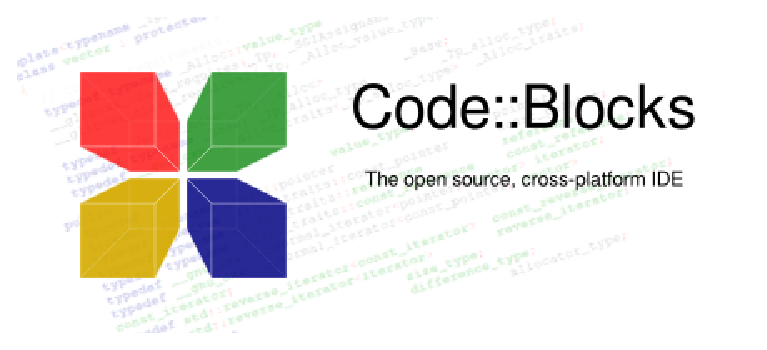
\includegraphics[width=\columnwidth]{mystyles/cb_splash}
    \vfill
    \makeatletter
    \@ifundefined{Subtitle}{%
        {\Huge\textbf{\Subject}\\ [2ex] \Title\\ [2ex] \large{Version \DocVersion}\\ [2ex]}
    }{%
        {\Huge\textbf{\Subject}\\ [2ex] \Title\\ \Subtitle\\ [2ex] \large{Version \DocVersion}\\ [2ex]}
    }
    \makeatother
    \vfill
    Merci à l'équipe \codeblocks  :\\

    Anders F. Björklund (afb), Biplab Kumar Modak (biplab), Bartomiej wiecki (byo),
    Paul A. Jimenez (ceniza), Koa Chong Gee (cyberkoa), Daniel Orb (daniel2000), Lieven de Cock (killerbot), Yiannis Mandravellos (mandrav), Mispunt (mispunt), Martin Halle (mortenmacfly), Jens Lody (jens), Jerome Antoine (dje), Damien Moore (dmoore),
    Pecan Heber (pecan), Ricardo Garcia (rickg22), Thomas Denk (thomasdenk), tiwag (tiwag), stahta01 (stahta01), Teodor Petrov (oBFusCATed), BlueHazzard (BlueHazzard), Andrew Cottrell (AndrewCot), Miguel Gimenez (wh11204) 

    Et bien d'autres contributeurs...

    Manuel original en Anglais et en Allemand (V1.x) par Mario Cupelli (mariocup)\\
    Traduction en français de la version originale anglaise et corrections/ajouts dans la version 2 par Gérard Durand (gd\_on).\\
    Quelques paragraphes sont directement recopiés depuis le WiKi de \codeblocks. N'hésitez pas à le visiter sur \url{https://wiki.codeblocks.org/index.php/Main_Page}, les informations y sont peut-être plus à jour.\\

    Il est permis de copier, distribuer et/ou modifier ce document dans le respect de la licence "GNU Free Documentation", Version 1.2 ou toute autre version postérieure publiée par la "Free Software Foundation".

    Manuel Utilisateur mis à jour en novembre 2022
    \end{flushleft}
    \end{titlepage}
    \pagestyle{headings}
%%%%%%%%%%%% Table of contents %%%%%%%%%%%%%%%%%%%%%%%%%%%%%%%%%%%%%%%%%%%
% This ifthenelse is desactivated, because it has problems with recent Miktex versions (22.10), though it was OK with a previous one (22.03).
% More, it's only used when shortdocu is false, which is not the standard case for C::B documentation.
%    \ifthenelse{\boolean{shortdocu}}{}{
%%        \tableofcontents
%        \ifthenelse{\boolean{figreg}}{\listoffigures}{}
%        \ifthenelse{\boolean{tabreg}}{\listoftables}{}
%    }
    \clearemptydoublepage \pagestyle{headings}
    \pagenumbering{arabic}
}{%
    \begin{titlepage}
        \@ifundefined{Subtitle}{%
            \Huge\textbf{{\Subject} {\Title}}\\
        }{
            \Huge\textbf{{\Subject} {\Title} {\Subtitle}}\\
        }
        \large{Version \DocVersion}
    \end{titlepage}
    \clearemptydoublepage \pagestyle{headings}
    %\tableofcontents
    \clearemptydoublepage \pagenumbering{arabic}
    \pagenumbering{arabic}
}
\makeatother

\ifhtml
	% No tableofcontents
\else
	\tableofcontents{}
\fi
\chapter{Gestion de Projet \codeblocks}

Les textes de plusieurs paragraphes (par exemple le chapitre \pxref{sec:variables_types} ou la \pxref{sec:plugins}) sont les documentations officielles du site Wiki de \codeblocks (éventuellement revues et complétées) où elles ne sont disponibles qu'en anglais.
Cette documentation est une extension de la version originale 1.1, assemblée et/ou écrite par Mario Cupelli.

\hint{Remarque du traducteur : 
Les références aux menus sont traduites en français. Cela suppose donc que vous avez installé la francisation de l'interface de \codeblocks que vous pouvez obtenir, notamment via le forum, dans la rubrique CodeBlocks Translation. Ne plus utiliser celle du site original LaunchPad bien trop ancienne et largement dépassée. Utiliser plutôt une nouvelle version, aussi sur Launchpad, via \url{https://launchpad.net/codeblocks-gd}. Les images ci-dessous sont celles de la documentation originale, en anglais}

L'illustration ci-dessous montre l'apparence de la fenêtre de l'interface utilisateur de \codeblocks.

\figures[H][width=\columnwidth]{codeblocks}{Environnement de développement Intégré (IDE) de \codeblocks}

\begin{description}
\item[Gestion] Cette fenêtre contient l'interface \menu{Projets} qui dans le texte suivant sera référencée comme vue du projet. Cette vue affiche tous les projets ouverts dans \codeblocks à un instant donné. L'onglet \samp{Symboles} de la fenêtre Gestion affiche les symboles, les variables etc.
\item[Éditeur] Dans l'illustration ci-dessus, un fichier source nommé \file{hello.c} est ouvert avec colorisation de syntaxe dans l'éditeur.
\item[Liste des fichiers ouverts] affiche une liste de tous les fichiers ouverts dans l'éditeur, dans cet exemple : \file{hello.c}.
\item[CodeSnippets] peut être affiché via le menu \menu{Vue, CodeSnippets}. Ici vous pouvez gérer des modules de texte, des liens vers des fichiers et des liens vers des urls.
\item[Journaux \& autres]. Cette fenêtre est utilisée pour sortir des résultats de recherche, des messages envoyés par un compilateur etc..
\end{description}

La barre d'état donne un aperçu des paramétrages suivants :

\begin{itemize}
\item Chemin absolu d'un fichier ouvert dans l'éditeur.
\item L'éditeur utilise l'encodage par défaut de votre système d'exploitation. Cette configuration sera affichée par défaut.
\item Numéros de ligne et de colonne de la position actuelle du curseur dans l'éditeur.
\item Le mode de configuration du clavier pour insérer du texte (Insertion ou Remplacement).
\item État actuel du fichier. Un fichier modifié sera marqué comme \codeline{Modifie} sinon cette case reste vide. 
\item Autorisation d'un fichier. Un fichier qui est en lecture seule sera affiché \codeline{Lecture seule} dans la barre d'état. Dans la fenêtre \menu{Ouvrir la liste de fichiers} ces fichiers seront identifiés par une icône de verrouillage superposée.

\hint{Dans l'éditeur courant, l'utilisateur peut choisir les propriétés du menu de contexte. Dans le dialogue apparaissant dans l'onglet \menu{Général}, l'option \menu{Le fichier est en lecture seule} peut être sélectionnée. Cette option marquera le fichier correspondant comme étant en lecture seule pour \codeblocks, mais les attributs en lecture et écriture du fichier original ne seront pas modifiés dans le système de fichiers.}

\item Si vous démarrez \codeblocks en ligne de commande avec \opt{--personality=\var{profile}} la barre d'état affichera le profil utilisateur courant, sinon \codeline{default} sera affiché. Les paramètres de \codeblocks sont enregistrés dans le fichier de configuration correspondant \file{\var{personality}.conf}.
\end{itemize}

\codeblocks offre une gestion des projets très flexible et très compréhensible. Le texte suivant ne montre que quelques aspects de la gestion de projets.

\section{Vue du projet}\label{sec:categories}

Dans \codeblocks, les sources et les paramètres d'un processus de génération sont stockés dans un fichier projet \file{\var{name}.cbp}. Les sources en C/C++ et les fichiers d'en-têtes correspondants (ou headers) sont les composants typiques d'un projet. La façon la plus simple de créer un projet est de passer par la commande \menu{Fichier,Projet} et de choisir un assistant. Vous pouvez alors ajouter des fichiers au projet via le menu de contexte \menu{Ajouter des fichiers} de la fenêtre de gestion. 

\codeblocks gère les fichiers de projets en catégories qui dépendent de l'extension des fichiers. Les catégories suivantes sont prédéfinies :

\begin{description}
\item[Sources] contient les fichiers sources dont l'extension est \file{*.c;*.cpp;}.
\item[ASM Sources] contient les fichiers sources dont l'extension est \file{*.s;*.S;*.ss;*.asm}.
\item[Headers] contient, entre autres, les fichiers dont l'extension est \file{*.h;}.
\item[Ressources] contient les fichiers pour paramétrer l'aspect des fenêtres des wxWidgets avec les extensions \file{*.res;*.xrc;}. Ces types de fichiers sont affichés dans l'onglet \samp{Ressources} de la fenêtre de Gestion.
\end{description}

Les paramètres des types et catégories de fichiers peuvent être ajustés via le menu de contexte \menu{Arbre des projets,Éditer les types et catégories de fichiers}. Ici, vous pouvez définir aussi des catégories personnalisées pour les extensions de votre choix. Par exemple, si vous souhaitez lister des scripts d'édition de liens avec l'extension \file{*.ld} dans une catégorie nommée \file{Linkerscript}, vous n'avez qu'à créer une nouvelle catégorie.

\hint{Si vous désactivez \menu{Arbre des projets,Catégoriser par type de fichiers} dans le menu de contexte, l'affichage par catégories sera masqué, et les fichiers seront listés comme ils sont stockés dans le système de fichiers.}

\section{Notes pour les Projets}

Dans \codeblocks, des notes spécifiques peuvent être stockées dans un projet. Ces notes peuvent contenir de brèves descriptions ou des points particuliers pour le projet correspondant. En affichant ces informations à l'ouverture d'un projet, les autres utilisateurs peuvent avoir un rapide aperçu de l'avancement du projet. L'affichage des notes peut être validé ou invalidé via l'onglet Notes des Propriétés d'un projet.

\section{Modèles de Projet}

\codeblocks est fourni avec tout un ensemble de modèles de projets qui sont affichés quand on crée un nouveau projet. Cependant, vous pouvez aussi enregistrer des modèles personnalisés pour y sauvegarder vos propres spécifications d'options de compilation, les optimisations à utiliser, les options spécifiques aux machines etc. Ces modèles seront enregistrés dans \file{Documents and Settings\osp \var{user}\osp Application Data\osp codeblocks\osp UserTemplates} sous Win 7 (ou un chemin équivalent du profil de l'utilisateur, adapté à chaque OS). Si les modèles doivent pouvoir être ouverts par tous les utilisateurs, ils devront être copiés dans un répertoire correspondant de l'installation de \codeblocks. Ces modèles seront alors affichés lors du démarrage suivant de \codeblocks dans \menu{Nouveau,Projet,Modèles utilisateur}.

\hint{Les modèles disponibles dans l'assistant Projet peuvent être édités en les sélectionnant via un clic droit.}

\section{Créer des Projets à partir de Cibles de Génération}

Dans les projets, il est nécessaire d'avoir à disposition différentes variantes de projets. On appelle ces variantes Cibles de Génération. Elles diffèrent par leurs options de compilation, les informations de débogage et/ou le choix des fichiers. Une cible de génération peut aussi être externalisée dans un projet séparé. Pour ce faire, cliquer sur \menu{Projet,Propriétés} puis sélectionner la variante dans l'onglet \samp{Générer les cibles} et cliquer sur le bouton \samp{Créer un projet à partir d'une cible} (voir \pxref{fig:build_targets}).

\screenshot{build_targets}{Cibles de Génération}

\section{Cibles Virtuelles}

Les projets peuvent être également structurés dans \codeblocks en ce qu'on appelle des cibles virtuelles. Une structure fréquemment utilisée de projet consiste en deux cibles de génération, la première cible \samp{Debug} qui contient des informations pour le débogage et la seconde cible \samp{Release} sans ces informations. En ajoutant Cibles Virtuelles via \menu{Projet,Propriétés,Cibles de génération} on peut combiner des cibles de génération individuelles. Par exemple, une Cible Virtuelle \samp{All} peut créer les cibles Debug et Release simultanément. Les cibles virtuelles sont affichées dans la barre de symboles du compilateur dans Générer les cibles.

\section{Étapes Pré- et Post Génération}\label{sec:pre_postbuild}

Dans \codeblocks on peut effectuer des opérations complémentaires avant et après la compilation d'un projet. Ces opérations sont appelées étapes de Pré génération ou Post génération. Des Post générations typiques sont :

\begin{itemize}
\item Création d'un format Intel Hexformat à partir un objet terminé
\item Manipulation d'objets par \cmdline{objcopy}
\item Générer des fichiers de dump par \cmdline{objdump}
\end{itemize}

\genterm{Exemple}

Créer le désassemblage d'un objet sous Windows. Le transfert vers un fichier nécessite l'appel à \cmdline{cmd} avec l'option \opt{/c}.

\begin{lstlisting}
cmd /c objdump -D name.elf > name.dis
\end{lstlisting}

Un autre exemple de Post génération peut être l'archivage d'un projet. Pour cela, créez une cible de génération \samp{Archive} et incluez les instructions suivantes dans l'étape de post génération :

\begin{lstlisting}
zip -j9 $(PROJECT_NAME)_$(TODAY).zip src h obj $(PROJECT_NAME).cbp
\end{lstlisting}

Avec cette commande, le projet actif et ses sources, en-têtes et objets seront compressés en tant que fichier zip. En faisant ainsi, les variables intégrées \codeline{$(PROJECT_NAME)} et \codeline{$(TODAY)}, le nom du projet et la date courante seront extraites (voir \pxref{sec:builtin_variables}). Après l'exécution de la cible \samp{Archive}, le fichier compressé sera stocké dans le répertoire du projet.

Dans le répertoire \file{share/codeblocks/scripts} vous trouverez quelques exemples de scripts. Vous pouvez ajouter un script via le menu \menu{Paramètres,Édition de scripts} et l'enregistrer dans un menu. Si vous exécutez par exemple le  script \file{make\_dist} depuis le menu, alors tous les fichiers appartenant à un projet seront compressés dans une archive \file{\var{project}.tar.gz}.

\section{Ajouter des Scripts à des Cibles de Génération}

\codeblocks offre la possibilité d'utiliser des actions de menus dans les scripts. Le script représente un autre degré de liberté pour contrôler la génération de votre projet.

\hint{Un script peut également être inclus dans une Cible de Génération.}

\section{Espace de travail et Dépendances de Projet}

Des projets multiples peuvent être ouverts dans \codeblocks. En enregistrant les projets ouverts via  \menu{Fichier,Enregistrer l'espace de travail} vous pouvez les rassembler dans un seul espace de travail sous \file{\var{name}.workspace}. Si vous ouvrez \file{\var{name}.workspace} au démarrage suivant de \codeblocks, tous les projets seront de nouveau affichés.

Les logiciels complexes sont un assemblage de composants qui sont gérés dans différents projets \codeblocks. De plus, lors de la génération de tels logiciels, il y a souvent des dépendances entre ces projets.

\genterm{Exemple}

Un projet A contient des fonctions de base qui sont rendues disponibles aux autres projets sous forme d'une librairie. Maintenant, si les sources de ce projet sont modifiées, alors la librairie doit être re-générée. Afin de maintenir la consistance entre un projet B qui utilise ces fonctions et le projet A qui les implémente, le projet B doit dépendre du projet A. Les informations nécessaires aux dépendances des projets sont enregistrées dans l'espace de travail adéquat, ainsi chaque projet peut être généré séparément. L'utilisation des dépendances rend également possible le contrôle de l'ordre dans lequel sont générés les projets. Les dépendances de projets peuvent être configurées en sélectionnant le menu \menu{Projet,Propriétés} puis en cliquant sur le bouton \samp{Dépendances du projet}.

\section{Inclure des Fichiers en Assembleur}

Dans la fenêtre Gestion d'une vue de projet, les fichiers en Assembleur sont affichés dans la catégorie \file{ASM Sources}. L'utilisateur peut changer la liste des fichiers dans les catégories (voir \pxref{sec:categories}). Un clic droit sur un des fichiers assembleur listés ouvrira un menu de contexte. Sélectionner \menu{Propriétés} pour ouvrir une nouvelle fenêtre. Sélectionnez maintenant l'onglet \samp{Générer} et activez les deux champs  \samp{Compiler le fichier} et \samp{Édition de liens du fichier}. Sélectionnez ensuite l'onglet \samp{Avancé} et exécutez les étapes suivantes :

\begin{enumerate}
\item Configurer \samp{Variable de compilation} à CC
\item Sélectionner le compilateur dans \samp{Pour ce compilateur}
\item Sélectionner \samp{Utiliser des commandes personnalisées pour générer ce fichier}
\item Dans la fenêtre, entrez :
\begin{lstlisting}
$compiler $options $includes <asopts> -c $file -o $object
\end{lstlisting}
\end{enumerate}

Les variables de \codeblocks sont identifiées par un \codeline{$} (voir \pxref{sec:command_macros}). Elles sont automatiquement configurées, ainsi vous n'avez à remplacer que l'option de l'assembleur \var{asopt} par vos propres configurations.


\section{Éditeur et Outils}
\begin{samepage}
Cette section regroupe des fonctions internes à l'éditeur

\subsection{Code par Défaut}
\end{samepage}

Les règles de codage dans une compagnie imposent d'avoir un modèle standard. Avec \codeblocks, il est possible d'inclure un contenu prédéfini automatiquement en début de fichier lors de la création d'une nouvelle source C/C++ ou d'en-têtes (headers). Le contenu prédéfini est dénommé code par défaut. Cette configuration peut être sélectionnée dans  \menu{Paramètres,Éditeur} Code par Défaut. Si vous créez un nouveau fichier alors une expansion des variables macro, notamment celles de \menu{Paramètres,Variables Globales}, est effectuée. Un nouveau fichier peut être créé via le menu \menu{Fichier,Nouveau,Fichier}.

\genterm{Exemple}

\begin{lstlisting}
/***************************************************************
 *  Project: $(project)
 *  Function:
 ***************************************************************
 *  $Author: mario $
 *  $Name:  $
 ***************************************************************
 *
 *  Copyright 2007 by company name
 *
 ***************************************************************/
\end{lstlisting}

\subsection{Abréviations}\label{sec:Abbreviations}

Pas mal de frappes au clavier peuvent être économisées dans \codeblocks en définissant des abréviations. Ceci peut s'obtenir en sélectionnant \menu{Paramètres,Éditeur} et en définissant les abréviations par un nom \var{name}, qui peut alors être appelé par un raccourci clavier Ctrl-J (voir \pxref{fig:abbreviation}).

\screenshot{abbreviation}{Définition des abréviations}

On peut également les paramétrer en incluant des variables \codeline{$(NAME}) dans les abréviations.

\begin{lstlisting}
#ifndef $(Guard token)
#define $(Guard token)
#endif // $(Guard token)
\end{lstlisting}

Quand on utilise l'abréviation \var{name} dans un texte source et qu'on utilise Ctrl-J, le contenu de la variable est récupéré puis inclus.
%Inherit Class
%Im Editor kann durch Auswahl von Inherit Class über die rechte Maustaste. ???

\subsection{Personnalités}\label{sec:personalities}

Les configurations de \codeblocks sont enregistrées en tant que données d'application dans un fichier dénommé \file{\var{user}.conf} dans le répertoire de \file{codeblocks}. Ce fichier de configuration contient des informations telles que les derniers projets ouverts, le paramétrage de l'éditeur, l'affichage des barres de symboles etc. Par défaut, la personnalité \samp{default} est utilisée et sa configuration sauvegardée dans un fichier \file{default.conf}. Si \codeblocks est lancé en ligne de commande avec le paramètre \cmdline{--personality=myuser}, le paramétrage sera enregistré dans un fichier \file{myuser.conf}. Si le profil n'existe pas déjà, il sera automatiquement créé. Cette procédure rend possible la création de différents profils pour différentes étapes de travail. Si vous lancez \codeblocks en ligne de commande avec le paramètre additionnel \cmdline{--personality=ask}, une boîte de sélection sera affichée avec tous les profils disponibles.

\hint{Le nom du profil/personnalité courant est affiché dans le coin à droite de la barre d'état.}

\subsection{Fichiers de Configuration}

Les paramètres de \codeblocks sont enregistrés dans le fichier de profil \file{default.conf} dans le répertoire \file{codeblocks} de votre Application Data. Quand vous utilisez des personnalités (ou profils) (voir \pxref{sec:personalities}), les détails de configuration sont enregistrés dans un fichier \file{\var{personality}.conf}.

L'outil \cmdline{cb\_share\_conf}, qu'on trouve dans le répertoire d'installation de \codeblocks, est utilisé pour gérer et enregistrer ces paramétrages.

Si vous souhaitez définir des paramètres standard pour plusieurs utilisateurs de l'ordinateur, le fichier de configuration \file{default.conf} doit être enregistré dans le répertoire \file{\osp Documents and Settings\osp Default User\osp Application Data\osp codeblocks}. Lors du premier démarrage, \codeblocks copiera les valeurs par défaut depuis  \samp{Default User} vers le répertoire "Application data" de l'utilisateur courant.

Pour créer une version portable de \codeblocks sur clé USB, procédez comme suit. Copiez le répertoire d'installation de \codeblocks vers la clé USB et stockez le fichier de configuration \file{default.conf} dans ce répertoire. Cette configuration servira de paramétrage global. Faites attention au fait que ce fichier soit accessible en écriture, sinon les changements de configuration ne pourront y être enregistrés.

\subsection{Navigation et Recherche}

Dans \codeblocks il y a plusieurs façons de naviguer rapidement entre les fichiers et les fonctions. Une procédure typique est la configuration de marques de recherche. Via le raccourci clavier Ctrl-B une marque est posée ou supprimée dans un fichier source. Via Alt-PgUp vous pouvez aller à la marque précédente, et via Alt-PgDn vous pouvez aller à la marque suivante.

Si vous sélectionnez l'espace de travail ou un projet particulier de l'espace de travail dans la vue du projet vous pouvez rechercher un fichier dans le projet. Sélectionnez tout simplement \menu{Rechercher le fichier} depuis le menu de contexte, puis tapez le nom du fichier et le fichier sera sélectionné. Si vous tapez sur la touche Entrée, ce fichier sera ouvert dans l'éditeur (voir \pxref{fig:project_find_file}).

\screenshot[H][width=.45\columnwidth]{project_find_file}{Recherche de fichiers}

Dans \codeblocks vous pouvez facilement naviguer entre les En-têtes/Sources en :

\begin{enumerate}
\item Positionnant le curseur à l'endroit où le fichier d'en-tête (header) est inclus puis ouvrir ce fichier via le menu de contexte \menu{Ouvrir le fichier inclus} (voir \pxref{fig:open_header})
\item Basculer du fichier d'en-tête au fichier source via le menu de contexte \menu{Basculer en-tête/source}
\item Sélectionner par exemple un define dans l'éditeur et choisir \menu{Trouver la déclaration} depuis le menu de contexte pour ouvrir le fichier contenant cette déclaration.
\end{enumerate}

\screenshot{open_header}{Ouverture d'un fichier d'en-têtes}

\codeblocks offre plusieurs possibilités de recherches dans un fichier ou un répertoire. La boîte de dialogue de recherche s'ouvre par \menu{Chercher,Rechercher} (Ctrl-F) ou \menu{Rechercher dans les fichiers} (Ctrl-Shift-F).

Alt-G et Ctrl-Alt-G sont d'autres fonctions utiles. Le dialogue qui s'ouvrira en utilisant ces raccourcis vous permet de choisir des fichiers/fonctions et aller vous positionner à l'implémentation de la fonction sélectionnée (voir \pxref{fig:select_function}) ou bien ouvrir le fichier sélectionné dans l'éditeur. Vous pouvez utiliser dans le dialogue des jokers comme \codeline{*} ou \codeline{?} etc. pour y obtenir une recherche incrémentale.

\screenshot[!hbt][width=.5\columnwidth]{select_function}{Recherche de fonctions}

\hint{Avec le raccourci Ctrl-PgUp vous pouvez aller à la fonction précédente, et via Ctrl-PgDn vous pouvez aller à la fonction suivante.}

Dans l'éditeur, vous pouvez ouvrir un nouveau dialogue Ouvrir des fichiers Ctrl-Tab et vous pouvez passer de l'un à l'autre via la liste affichée. Si vous appuyez sur la touche Ctrl, alors un fichier peut être sélectionné de différentes façons :

\begin{enumerate}
\item Si vous sélectionnez une entrée avec le bouton gauche de la souris, le fichier sélectionné sera ouvert.
\item Si vous appuyez sur la touche Tab vous passez de l'une à l'autre des entrées listées. En relâchant la touche Ctrl le fichier sélectionné sera ouvert.
\item Si vous déplacez la souris au-dessus des entrées listées, alors la sélection courante sera surlignée. En relâchant la touche Ctrl le fichier sélectionné sera ouvert..
\item Si le pointeur de souris est en dehors de la sélection surlignée, vous pouvez utiliser la molette de la souris pour basculer entre les entrées. En relâchant la touche Ctrl le fichier sélectionné sera ouvert.
\end{enumerate}

Une façon commune de développer du logiciel est de jongler avec un ensemble de fonctions implémentées dans différents fichiers. L'extension "Browse Tracker" vous aidera à résoudre cette tâche en vous montrant dans quel ordre ont été sélectionnés les fichiers. Vous pouvez alors naviguer aisément entre les appels de fonctions (voir \pxref{sec:browsetracker}).

L'affichage des numéros de lignes dans \codeblocks peut s'activer via \menu{Paramètres,Éditeur,Paramètres généraux} à l'aide du champ \samp{Afficher les numéros de ligne}. Le raccourci Ctrl-G ou la commande de menu \menu{Rechercher,Aller à la ligne} vous aidera à atteindre la ligne désirée.

\hint{Si vous maintenez la touche Ctrl enfoncée en sélectionnant du texte dans l'éditeur de \codeblocks vous pouvez lancer une recherche Internet, notamment avec Google, via le menu de contexte.}

\subsection{Vue des Symboles}

La fenêtre Gestion de \codeblocks offre une vue arborescente des symboles des sources en C/C++ pour naviguer dans les fonctions et les variables. Dans ce type de vue, vous pouvez travailler sur le fichier courant, le projet courant ou tout l'espace de travail.

\hint{Entrer un terme à chercher ou des noms de symboles dans le masque d'entrée 'Rechercher' du navigateur de Symboles permet d'obtenir une vue filtrée des symboles si concordance il y a.}

Les catégories suivantes existent pour les symboles :

\begin{description}
\item[Fonctions Globales] Liste l'implémentation des fonctions globales.
\item[typedefs globales] Liste l'utilisation des définitions \codeline{typedef}.
\item[Variables globales] Affiche les symboles de variables globales.
\item[Symboles du pré-processeur] Liste les directives du pré-processeur créées par \codeline{#define}.
\item[Macros globales] Liste les macros des directives du pré-processeur
\end{description}

\figures[H][width=.3\columnwidth]{symbols}{Vue des symboles}

Les structures et classes sont affichées par le menu \menu{arbre du bas} et l'ordre de tri peut être modifié via le menu de contexte. Si une catégorie est sélectionnée à la souris, les symboles trouvés seront affichés dans la partie basse de la fenêtre (voir \pxref{fig:symbols}). Double-cliquer sur un symbole ouvrira le fichier où il est défini ou bien la fonction où elle est implémentée, puis on se positionnera sur la ligne correspondante. Un rafraîchissement automatique du navigateur de symboles, sans avoir à sauvegarder de fichier, peut être activé par le menu \menu{Paramètres,Éditeur,Code Complétion} (voir \pxref{fig:cc_realtime_parsing}). Les performances de \codeblocks seront affectées dans les projets comportant de nombreux symboles.

\figures[H][width=.85\columnwidth]{cc_realtime_parsing}{Activation de l'analyse en temps réel}

\hint{Dans l'éditeur, une liste de classes peut être affichée via les menus de contexte \menu{Insérer méthode de classe} ou \menu{Toutes méthodes de classes sans implémentation}.}

\subsection{Inclure des Fichiers d'Aide Externes}

\codeblocks est seulement fourni avec son propre fichier d'aide : normalement, les développeurs ont besoin de bien plus d'aides et de références pour les langages, les librairies, les protocoles, les formats de fichiers et ainsi de suite. Le plugin help rend accessible toute la documentation nécessaire depuis \codeblocks lui-même. Virtuellement, tout document peut être interprété par le système d'aide de \codeblocks, depuis que le "plugin help" a la possibilité, si besoin, de lancer des programmes externes pour visualiser les documents ajoutés.

Une fois qu'a été ajouté un nouveau fichier ou document d'aide, une nouvelle entrée dans le menu "Aide" est disponible afin de pouvoir l'ouvrir.

L'environnement de développement \codeblocks supporte l'inclusion de fichiers d'aide externes via le menu \menu{Paramètres,Environnement}. Insérez le manuel de votre choix (au format chm par ex., voir ci-dessous) dans la sélection \menu{Fichiers d'aide}, sélectionnez \samp{Ceci est le fichier d'Aide par défaut} (voir \pxref{fig:help_files}). L'entrée \codeline{$(keyword)} est un paramètre de substitution pour une sélection particulière dans votre éditeur. Vous pouvez alors sélectionner une fonction dans un fichier ouvert de \codeblocks par un simple clic, et la documentation correspondante s'affichera lorsque vous appuierez sur la touche F1.

Si vous avez inclus plusieurs fichiers d'aide, vous pouvez choisir un terme particulier dans l'éditeur, puis choisir le fichier d'aide adéquat dans le menu de contexte \menu{Chercher dans} pour que \codeblocks y fasse la recherche.

\screenshot{help_files}{Configuration des fichiers d'aide}

Dans \codeblocks vous pouvez également ajouter un support de pages "man". Ajoutez seulement une entrée \menu{man} et spécifiez les chemins comme suit (NdT ici pour Linux!).

\begin{lstlisting}
man:/usr/share/man
\end{lstlisting}

Sous Linux, les pages man sont habituellement installées de toute façon. Sous Windows vous pourriez vouloir les télécharger, par ex. depuis ici : \url{https://www.win.tue.nl/~aeb/linux/man}

\textbf{Options d'Aide}

\begin{itemize}
\item Vous pouvez demander à \codeblocks d'utiliser un fichier particulier comme fichier d'aide par défaut, en cochant la case "Ceci est le fichier d'aide par défaut". Ainsi, ce fichier sera affiché dès lors que vous appuierez sur la touche 'F1'. De plus, si vous écrivez le mot \$(keyword) en tant que mot clé par défaut (voir plus loin), on cherchera ces mots clés dans ce fichier (le mot sélectionné ou le mot sous le curseur du fichier source courant) et les correspondances seront affichées, si elles existent.

\item Vous pouvez demander à \codeblocks d'ouvrir un fichier d'aide sur un sujet de votre choix, en écrivant le mot clé correspondant dans la boîte de texte "Valeur du mot clé par défaut". Si le fichier d'aide est celui par défaut et que vous utilisez \$(keyword) comme mot clé par défaut, l'éditeur utilisera le mot sous le curseur (ou celui sélectionné) dans le fichier d'aide actuellement ouvert comme mot clé, en ouvrant le fichier d'aide par défaut sur le sujet adéquat. Ceci ne sera toutefois vrai que sur le fichier d'aide par défaut : on ne cherchera pas de cette façon dans les autres fichiers d'aide. Par exemple, si vous avez une référence de langage comme fichier d'aide par défaut et que vous ajoutez un fichier d'aide sur une librairie standard, vous obtiendrez l'explication du mot clé du langage en appuyant sur la touche 'F1', mais vous n'aurez pas les fonctions de librairie expliquées de cette façon. Inversement, en configurant le fichier de la librairie par défaut, via la touche F1 vous perdrez cette fonctionnalité pour les mots clés de langage.

\item Si votre fichier d'aide est un fichier HTML, vous pouvez demander à \codeblocks de l'ouvrir avec le visualiseur de fichiers HTML intégré, en cochant l'option correspondante.
\end{itemize}

\codeblocks fourni un \samp{Visualiseur HTML intégré}, qui peut être utilisé pour afficher un simple fichier html et y rechercher des mots clés. Configurez simplement le chemin du fichier html qui doit être analysé et cochez la case  \menu{Ouvrir ce fichier avec le visualiseur d'aide intégré} via le menu \menu{Paramètres,Environnement,Fichiers d'aide}.

\screenshot{embedded_html_viewer}{Visualiseur HTML intégré}

\hint{Si vous sélectionnez un fichier html par double-clic dans l'explorateur (voir \pxref{sec:file_explorer}) alors le visualiseur html intégré sera démarré, du moins si aucune association vers les fichiers html n'est faite par le gestionnaire d'extensions de fichiers.}

\textbf{Fichiers CHM}

Vous pouvez trouver des fichiers d'aide c++ chm sur le web. Ajoutez-les tout simplement dans la boîte de dialogue.

Sous Linux vous avez à installer un visualiseur de fichiers chm pour pouvoir afficher ces fichiers chm. Il y en a plusieurs comme gnochm, kchmviewer, xchm et ainsi de suite. 

% \section{Scripting}
%
% \codeblocks in Console Modus + Scripts

\subsection{Inclure des outils externes}

L'inclusion d'outils externes dans \codeblocks est faisable via \menu{Outils,Configurer les outils,Ajouter}. Les variables internes (voir \pxref{sec:builtin_variables}) peuvent aussi être utilisées comme paramètres des outils. D'autre part, il y a plusieurs sortes d'options de lancement pour démarrer des applications externes. En fonction des options, les applications externes peuvent s'arrêter quand on quitte \codeblocks. Si les applications doivent rester ouvertes après qu'on ait quitté \codeblocks, l'option \menu{Lancer l'outil visible en mode détaché} doit être cochée.

\section{Astuces pour travailler avec \codeblocks}

Dans ce chapitre nous présenterons quelques paramétrages utiles dans \codeblocks.

\subsection{Recherche de Modifications}

\codeblocks fourni une fonctionnalité pour pister les modifications effectuées dans un fichier source et affiche une barre dans la marge là où ont eût lieu les changements. Les modifications sont marquées par une barre de changements jaune alors que celles qui ont déjà été enregistrées sont marquées par une barre de changements verte (voir \pxref{fig:changebar}). Vous pouvez naviguer dans vos changements à l'aide du menu  \menu{Rechercher,Aller à la ligne changée suivante} ou encore \menu{Rechercher,Aller à la ligne changée précédente}. La même fonctionnalité est accessible via les raccourcis clavier Ctrl-F3 et Ctrl-Shift-F3.

\screenshot{changebar}{Recherche de modifications}

Cette fonctionnalité peut être activée ou désactivée via la case à cocher \menu{Utiliser la barre de changements} dans le menu \menu{Paramètres,Éditeur,Marges et tirets}.

\hint{Si un fichier modifié est fermé, alors l'historique des changements tels que défaire/refaire ainsi que la barre de changements sont perdus. À l'aide du menu \menu{Édition,Effacer l'historique des changements} ou le menu de contexte correspondant vous pouvez effacer cet historique même si le fichier reste ouvert.}

\subsection{Échange de données avec d'autres applications}

Les échanges de données entre \codeblocks et d'autres applications sont possibles. Pour cela on utilise, avec Windows, le processus de communication inter processus DDE (Dynamic Data Exchange) et, avec les autres systèmes d'exploitation, une communication basée sur le protocole TCP.

Avec cette interface, différentes commandes peuvent être envoyées vers une instance de \codeblocks en suivant la syntaxe suivante.

\begin{lstlisting}
[<command>("<parameter>")]
\end{lstlisting}

Les commandes suivantes sont actuellement disponibles :

\begin{description}
\item[Open] La commande

\begin{lstlisting}
[Open("d:\temp\test.txt")]
\end{lstlisting}

utilise un paramètre, dans notre cas c'est le nom d'un fichier avec son chemin en absolu, et il s'ouvre dans une instance existante de \codeblocks ou bien, si nécessaire, une première instance démarre.
\item[OpenLine] Cette commande ouvre un fichier dans une instance de \codeblocks et se positionne sur la ligne dont le numéro est entré. Le numéro de ligne est spécifié par \codeline{:ligne}.

\begin{lstlisting}
[OpenLine("d:\temp\test.txt:10")]
\end{lstlisting}

\item[Raise] Donne le "focus" à l'instance de \codeblocks. Aucun paramètre ne doit être entré.
\end{description}

\subsection{Configurer les variables  d'environnement}\label{sec:EnvVars_Cfg}

Voir aussi l'"Extension Variables d'Environnement" dans la \pxref{sec:EnvVar_Plugin}.

La configuration d'un système d'exploitation se fait par ce qu'on appelle les variables d'environnement. Par exemple, la variable d'environnement \codeline{PATH} contient le chemin d'un compilateur installé. Le système d'exploitation analysera cette variable dans l'ordre d'écriture, c'est à dire que les entrées de la fin seront utilisées en dernier dans les recherches. Si plusieurs versions de compilateur ou d'autres applications sont installées, les situations suivantes peuvent se produire :

\begin{itemize}
\item On appelle une version incorrecte d'un logiciel
\item Les logiciels installés s'appellent entre eux
\end{itemize}

Ainsi, on peut tomber sur le cas où différentes versions d'un compilateur ou d'un autre outil sont obligatoires pour différents projets. Lorsque cela arrive, une première solution est de changer les variables d'environnement dans le système d'exploitation pour chaque projet. Toutefois cette procédure est sujette à erreur et manque de flexibilité. Pour ce faire, \codeblocks offre une solution élégante. Différentes configurations de variables peuvent être créées pour un usage uniquement en interne à \codeblocks. De plus, vous pouvez passer de l'une à l'autre de ces configurations. La \pxref{fig:env_variables} montre la boîte de dialogue que vous obtenez via \samp{Variables d'Environnement} dans \menu{Paramètres,Environnement}. On crée une configuration à l'aide du bouton \samp{Créer}.

\screenshot{env_variables}{Variables d'environnement}

L'accès et l'étendue des variables d'environnement ainsi créées sont limités à \codeblocks. Vous pouvez étendre ces variables d'environnement comme toutes les autres variables dans \codeblocks à l'aide de \codeline{$(NAME)}.

\hint{La configuration d'une variable d'environnement pour chaque projet peut être sélectionnée dans le menu de contexte \menu{Propriétés} de l'onglet \samp{Options EnvVars}.}

\genterm{Exemple}

Vous pouvez écrire dans un fichier \file{\var{project}.env} l'environnement utilisé dans une étape de post génération (voir \pxref{sec:pre_postbuild}) puis l'archiver dans votre projet.

\begin{lstlisting}
cmd /c echo \%PATH\%  > project.env
\end{lstlisting}

ou sous Linux

\begin{lstlisting}
echo \$PATH > project.env
\end{lstlisting}

\subsection{Basculer entre diverses dispositions}

En fonction des tâches à effectuer, il peut être utile d'avoir plusieurs configurations ou dispositions (ou présentations) différentes de  \codeblocks et de les sauvegarder. Par défaut, le paramétrage (notamment afficher/masquer les barres d'outils, aspect, etc.) est enregistré dans le fichier de configuration \file{default.conf}. En utilisant l'option en ligne de commande \opt{--personality=ask} au démarrage de \codeblocks, on peut choisir parmi plusieurs possibilités de paramétrages. En dehors de ces paramétrages globaux, il peut se produire une situation où vous souhaitez basculer entre différentes vues de fenêtres ou de barres de symboles pendant une session. L'édition de fichier et le débogage de projets sont deux exemples typiques de telles situations. \codeblocks offre un mécanisme pour enregistrer et sélectionner différentes dispositions afin d'éviter à l'utilisateur d'avoir à fermer et ouvrir manuellement et fréquemment des fenêtres et des barres de symboles. Pour enregistrer une disposition, sélectionnez le menu \menu{Vue,Disposition,Enregistrer la disposition actuelle} et entrez un nom dans \var{nom}. La commande \menu{Paramètres,Éditeur,Raccourcis clavier,Vue,Dispositions,\var{name}} permet de définir un raccourci clavier pour ce processus. Il est ainsi possible de basculer entre les diverses dispositions simplement en utilisant ces raccourcis clavier.

\hint{Autre exemple : éditer un fichier en mode plein écran sans barre de symboles. Vous pouvez créer une disposition comme \samp{Plein Ecran} et lui assigner un raccourci spécifique.}

\subsection{Basculer entre projets}

Si plusieurs projets ou fichiers sont ouverts en même temps, l'utilisateur a besoin d'un moyen pour passer rapidement de l'un à l'autre. \codeblocks possède plusieurs raccourcis pour ce faire.

\begin{description}
\item[Alt-F5] Active le projet précédent de la vue des projets.
\item[Alt-F6] Active le projet suivant de la vue des projets.
\item[F11] Dans l'éditeur, bascule entre un fichier source \file{\var{name}.cpp} et le fichier d'en-tête (header) correspondant \file{\var{name}.h}
\end{description}

\subsection{Configurations étendue des compilateurs}

Lors de la génération d'un projet, les messages du compilateur sont affichés dans l'onglet Messages de génération. Si vous souhaitez recevoir des informations détaillées, l'affichage peut être étendu. Pour cela, cliquez sur \menu{Paramètres,Compilateur et débogueur} puis sélectionnez l'onglet \samp{Autres options} dans le menu déroulant.

\screenshot{compiler_debugger}{Configurer des informations détaillées}

Assurez-vous que le compilateur soit correctement sélectionné. L'option \samp{Ligne de commande complète} des Avertissements du compilateur permet de sortir des informations détaillées. De plus, ces sorties peuvent être redirigées vers un fichier HTML. Pour cela, sélectionnez  \samp{Enregistrer le journal de génération dans un fichier HTML en fin de génération}.
D'autre part, \codeblocks peut afficher une barre d'avancement du processus de génération dans la fenêtre de génération qui peut être activée en cochant \samp{Afficher la barre de progression de génération}.

\subsection{Zoomer dans l'éditeur}

\codeblocks possède un éditeur très puissant. Cet éditeur vous permet de changer la taille des caractères du texte affiché des fichiers ouverts. Si vous avez une souris avec une molette, vous n'avez qu'à appuyer sur la touche Ctrl tout en tournant la molette dans un sens ou l'autre pour agrandir ou réduire la taille du texte.

\hint{Avec le raccourci Ctrl-Numepad-/ ou à l'aide du menu \menu{Édition,Commandes spéciales,Zoom,Remise à 0} vous restaurez la taille originale du texte courant.}

\subsection{Mode de Repliement}

Quand on édite des fichiers de texte, notamment des \file{*.txt}, dans \codeblocks, il peut être utile d'avoir le texte replié, ce qui signifie que les lignes longues seront affichées sur plusieurs lignes à l'écran afin qu'elles puissent être correctement éditées. La fonction \samp{Repliement} peut être activée dans \menu{Paramètres,Éditeur,Autres Options} ou en cochant la case \menu{Activer le repliement}. Les touches "Home" et "Fin" positionnent respectivement le curseur en début et en fin de ligne repliée. Quand on choisit \menu{Paramètres,Éditeur,Autres Options} et \menu{La touche Home déplace toujours le curseur en première colonne}, le curseur sera positionné respectivement en début ou en fin de ligne si on appuie sur la touche "Home" ou "Fin". Si on désire placer le curseur au début de la première ligne du paragraphe en cours, il vous faut utiliser la combinaison de touches \menu{Alt-Home}. La même chose de façon analogue pour \menu{Alt-Fin} pour positionner le curseur en fin de la dernière ligne du paragraphe courant.

\subsection{Sélection de modes dans l'éditeur}

\codeblocks supporte différents modes de sélection pour le couper-coller des chaînes de caractères.

\begin{enumerate}
\item Un texte de l'éditeur actif peut être sélectionné avec le bouton gauche de la souris, puis on relâche ce bouton. L'utilisateur peut se déplacer de haut en bas avec la molette de la souris. Si on appuie sur le bouton du milieu, le texte précédemment sélectionné sera inséré. Cet effet est disponible au niveau d'un fichier et peut être vu comme un presse-papier de fichier.
\item Appuyer sur la touche \samp{ALT} active ce qu'on appelle la sélection en mode bloc et un rectangle de sélection s'affiche à l'aide du bouton gauche de la souris. Lorsqu'on relâche la touche Alt cette sélection peut être copiée ou collée. Cette option est utile si vous voulez sélectionner des colonnes, notamment dans un tableau et en copier-coller le contenu.
\item Dans le menu \menu{Paramètres,Éditeur,Marges et tirets} on peut activer ce qu'on appelle des \menu{Espaces Virtuels}. Ceci active la possibilité d'avoir une sélection en mode bloc qui peut commencer ou se terminer par une ligne vide.
\item Dans le menu \menu{Paramètres,Éditeur,Marges et tirets} on peut activer le \menu{Sélections Multiples}. En maintenant enfoncée la touche Ctrl l'utilisateur peut sélectionner diverses lignes dans l'éditeur actif avec le bouton gauche de la souris. Les sélections sont ajoutées dans le presse-papier à l'aide des raccourcis Ctrl-C ou Ctrl-X. Ctrl-V en insèrera le contenu à la position courante du curseur. Une option complémentaire dénommée \menu{Active l'entrée clavier (et la suppression)}  peut être activée pour les sélections multiples. Cette option est utile si vous voulez ajouter des directives de pré-processeur comme \codeline{#ifdef} sur plusieurs lignes de code source ou si vous voulez superposer ou remplacer du texte en plusieurs endroits.
\end{enumerate}

\hint{La plupart des gestionnaires de fenêtres de Linux utilisent ALT-ClicGauche-Déplacer pour déplacer une fenêtre, aussi vous devrez désactiver cette fonctionnalité pour pouvoir sélectionner en mode bloc.}

\subsection{Repliement de code}

\codeblocks supporte ce qu'on appelle le repliement de code. Avec cette fonctionnalité vous pouvez replier notamment les fonctions dans l'éditeur de \codeblocks. Un point de repliement est marqué dans la marge gauche de
l'éditeur par un signe moins. Dans la marge, le début et la fin d'un point de repliement sont visibles à l'aide d'une ligne verticale. Si vous cliquez sur le signe moins avec le bouton gauche de la souris, la portion de code sera repliée ou dépliée. Via le menu \menu{Édition,Repliement} vous pouvez sélectionner le repliement. Dans l'éditeur, un code replié est vu comme une ligne horizontale continue.

\hint{Le style de repliement et la profondeur limite du repliement peuvent se configurer dans le menu \menu{Paramètres,Éditeur,Repliement}.}

\codeblocks fournit aussi la fonctionnalité de repliement pour les directives du pré-processeur. Pour l'activer, sélectionnez \samp{Replier les commandes du pré-processeur} dans l'entrée Repliement de \menu{Paramètres,Éditeur}.

Une autre façon de faire est de définir des points de repliement utilisateurs. Le point de départ du repliement s'entre comme un commentaire suivi d'une parenthèse ouvrante et la fin comme un commentaire suivi d'une parenthèse fermante.

\begin{verbatim}
//{
code avec repliement défini par l'utilisateur
//}
\end{verbatim}

\subsection{Auto complétion}

Lorsque vous ouvrez un projet dans \codeblocks les \samp{Répertoires de recherche} de votre compilateur et de votre projet, les fichiers sources et d'en-têtes de votre projet sont analysés. De plus les mots clés de l'analyseur syntaxique correspondant sont analysés également. Les informations issues de l'analyse sont alors utilisées pour la fonctionnalité d'auto complétion dans \codeblocks. Vérifiez s'il vous plait que cette fonctionnalité est bien activée dans l'éditeur. L'auto complétion est accessible au travers du raccourci Ctrl-Espace. Via le menu \menu{Paramètres,Éditeur,Colorisation syntaxique} vous pouvez ajouter des mots clés définis par l'utilisateur à votre analyseur syntaxique.

\subsection{Recherche de fichiers cassés}

Lorsqu'un fichier est supprimé du disque, mais est toujours inclus dans un fichier projet \file{\var{project}.cbp}, alors un \samp{fichier cassé} sera affiché avec un symbole "cassé" dans la vue du projet. Vous devriez utiliser  \menu{Enlever ce fichier du projet} plutôt que de supprimer le fichier.

Dans de gros projets, avec de nombreux sous-répertoires, la recherche de fichiers cassés peut être une grande consommatrice de temps. Avec l'extension ThreadSearch (voir \pxref{sec:thread_search}) \codeblocks apporte une solution simple à ce problème. Si vous entrez une expression de recherche dans ThreadSearch et sélectionnez l'option \menu{Fichiers du projet} ou \menu{Fichiers de l'espace de travail}, alors ThreadSearch analysera tous les fichiers qui sont inclus dans le projet ou l'espace de travail. Si un fichier cassé est trouvé, ThreadSearch génèrera une erreur sur le fichier absent.

\subsection{Inclure des librairies}

Dans les options de génération d'un projet, vous pouvez ajouter les librairies utilisées via le bouton \samp{Ajouter} dans l'entrée \samp{Librairies à lier} des \samp{Options de l'éditeur de liens}. Ce faisant, vous pouvez soit utiliser le chemin absolu de la librairie ou seulement donner son nom sans le préfixe \file{lib} ni l'extension du fichier.

\genterm{Exemple}

Pour une librairie nommée \file{\var{path}\osp libs\osp lib\var{name}.a}, écrire seulement \file{\var{name}}. L'éditeur de liens avec les chemins de recherche correspondants inclura alors correctement les librairies.

\hint{Une autre façon d'inclure des librairies est documentée dans la \pxref{sec:lib_finder}.}

\subsection{Ordre d'édition de liens des fichiers objets}

Lors de la compilation, les fichiers objets \file{name.o} sont créés à partir des sources \file{name.c/cpp}. L'éditeur de liens assemble les fichiers objets individuels pour en faire une application \file{name.exe} ou sur d'autre systèmes \file{name.elf}. Dans certains cas, il peut être préférable de prédéfinir l'ordre dans lequel seront liés les fichiers objets. Vous pouvez obtenir cela dans \codeblocks en assignant des priorités. Dans le menu de contexte \menu{Propriétés}, vous pouvez définir les priorités d'un fichier dans l'onglet Générer. Une priorité faible fera que le fichier sera lié plus tôt.

\subsection{Sauvegarde automatique}

\codeblocks offre la possibilité d'enregistrer automatiquement les projets et les fichiers sources, ou encore de créer des copies de sauvegarde. Cette fonctionnalité peut être activée dans le menu \menu{Paramètres,Environnement,Sauvegarde-auto}. Ce faisant, \samp{Enregistrer dans un fichier .save} doit être spécifié comme méthode de création de copie de sauvegarde.

\subsection{Configuration des extensions de fichiers}\label{sec:file_extension}

Dans \codeblocks, vous pouvez choisir entre plusieurs méthodes de traitement des extensions de fichiers. La boîte de dialogue de configuration s'ouvre par \menu{Paramètres,Gestion des extensions de fichiers}.
Vous pouvez alors soit utiliser les applications assignées par Windows pour chaque extension de fichier (l'ouvrir avec l'application associée), ou changer la configuration pour chaque extension de telle façon que ce soit un programme défini par l'utilisateur qui soit lancé (lancer un programme externe), ou que ce soit \codeblocks qui ouvre le fichier dans son éditeur (l'ouvrir dans l'éditeur de \codeblocks).

\hint{Si un programme utilisateur est associé à une certaine extension de fichier, la configuration \samp{Désactiver \codeblocks quand un programme externe est lancé} devrait être désactivée, sinon \codeblocks sera fermé dès qu'un fichier qui possède cette extension est ouvert.}

\section{\codeblocks en ligne de commande}

L'Environnement de Développement Intégré (IDE) \codeblocks peut être exécuté depuis une ligne de commande sans interface graphique. Dans ce cas, plusieurs options sont disponibles pour contrôler le processus de génération d'un projet. Comme \codeblocks peut être piloté par des "scripts", la création d'exécutables peut être intégrée dans vos propres processus de travail.

\begin{lstlisting}
codeblocks.exe /na /nd --no-splash-screen --build <name>.cbp --target='Release'
\end{lstlisting}

\begin{description}
\item[\var{filename}] Spécifie le nom du fichier de projet \file{*.cbp} ou le nom de l'espace de travail \file{*.workspace}. Par exemple, \var{filename} peut être \file{project.cbp}. Placez cet argument en fin de ligne de commande, juste avant la redirection de la sortie, s'il y en a une.
\item[--file=\var{filename}\optional{:ligne}] Ouvrir un fichier dans \codeblocks et, en option, se positionner sur une ligne particulière.
\item[/h, --help] Affiche un message d'aide concernant les arguments en ligne de commande.
\item[/na, --no-check-associations] Ne faire aucun contrôle d'association de fichiers (Windows seulement).
\item[/nd, --no-dde] Ne pas lancer le serveur DDE (Windows seulement).
\item[/ni, --no-ipc] Ne pas lancer le serveur IPC (Linux et Mac seulement).
\item[/ns, --no-splash-screen] Ne pas afficher l'écran de démarrage pendant le chargement de l'application.
\item[/d, --debug-log] Afficher le journal de débogage de l'application.
\item[--prefix=\var{str}] Configure le préfixe du répertoire de données partagées.
\item[/p, --personality=\var{str}, --profile=\var{str}] Configure le profil (ou personnalité) à utiliser. Vous pouvez utiliser le paramètre ask pour afficher la liste de tous les profils disponibles.
\item[--rebuild] Nettoie et génère le projet ou l'espace de travail.
\item[--build] Génère le projet ou l'espace de travail.
\item[--target=\var{str}] Configure la cible de génération. Par exemple \cmdline{--target='Release'}.
\item[--no-batch-window-close] Garde la fenêtre batch de journalisation visible après que la génération par batch soit terminée.
\item[--batch-build-notify] Affiche un message une fois que la génération batch est terminée.
\item[--safe-mode] Désactive toutes les extensions (plugins) au démarrage.
\item[$>$ \var{build log file}] Placé en toute dernière position d'une ligne de commande, ceci permet à l'utilisateur de rediriger la sortie standard vers un fichier log. Ceci n'est pas à proprement parler une option de codeblocks, mais seulement une redirection standard des sorties des shells DOS/*nix.
\end{description}

\section{Raccourcis Clavier}

Cette section décrit les raccourcis clavier qui sont ou peuvent être utilisés dans \codeblocks.

\subsection{Introduction}

Ce plugin peut être utilisé pour ajouter un ou plusieurs raccourcis clavier aux menus.

Même si une IDE comme \codeblocks est surtout pilotée à la souris, les raccourcis claviers sont néanmoins un moyen très pratique pour accélérer et simplifier le travail. Les tableaux ci-dessous regroupent quelques-uns des raccourcis claviers disponibles.

\subsection{Fonctionnalités}
\begin{description}
\item Inclue un panneau de configuration et un système complet pour visualiser/supprimer/ajouter/éditer des commandes en raccourcis clavier.
\item Supporte plusieurs profils de raccourcis clavier et un système complet de chargement/enregistrement est présent.
\item Permet à l'utilisateur de personnaliser toutes les commandes de menus désirées, et définir des raccourcis clavier pour chacune des commandes.
\end{description}

\subsection{Utilisation}

La page de configuration du plugin est accessible via le menu \menu{Paramètres,Éditeur}, en sélectionnant la section Raccourcis Clavier.

\screenshot{KeyBindConfig}{Dialogue de configuration des Raccourcis clavier}

Sélectionner une commande dans l'arborescence des Commandes, vous affiche le raccourci actuel pour la commande sur la droite. Sur la figure c'est Open... qui est sélectionné et le raccourci par défaut Ctrl-O est affiché.

Pour ajouter un nouveau raccourci à la commande sélectionnée, suivre les étapes suivantes :

\begin{enumerate}
\item Placer le curseur dans la boîte de texte au-dessous du Nouveau raccourci et presser sur les touches, par exemple F3 ou Ctrl-A.
\item Vérifier l'assignation courante, et si une autre commande a déjà ce raccourci affecté vous verrez son nom ici. Si le texte dit Aucun c'est que c'est bon.
\item Presser sur Ajouter pour ajouter le raccourci à la liste.
\item Presser sur OK dans le dialogue pour enregistrer des changements et retourner dans l'éditeur.
\end{enumerate}

\subsection{Éditeur}

{\small
\begin{longtable}{|l|l|}\hline
\textbf{Fonction}		        &	\textbf{Raccourci clavier}  \\ \hline
\endhead    % Pour répéter la ligne de titre si besoin
Défaire la dernière action 	    &	Ctrl+Z                      \\ \hline
Refaire la dernière action 	    &	Ctrl+Shift+Z                \\ \hline
Couper le texte sélectionné     &   Ctrl+X                      \\ \hline
Copier le texte sélectionné     &   Ctrl+C                      \\ \hline
Coller le texte                 &   Ctrl+V                      \\ \hline
Sélectionner tout le texte      &   Ctrl+A                      \\ \hline
Permuter en-têtes / source 	    &	F11                         \\ \hline
Commenter le code surligné      &	Ctrl+Shift+C                \\ \hline
Décommenter le code surligné    & 	Ctrl+Shift+X                \\ \hline
Dupliquer la ligne où est le curseur      & 	Ctrl+D          \\ \hline
Auto-complète / Abréviations    & 	Ctrl+Space/Ctrl+J           \\ \hline
Afficher les astuces            &	Ctrl+Shift+Space            \\ \hline
Permuter la ligne où est le curseur avec celle au-dessus    &	Ctrl+T\\ \hline
Bascule la marque 	            &	Ctrl+B                      \\ \hline
Aller à la marque précédente 	&	Alt+PgUp                    \\ \hline
Aller à la marque suivante  	&	Alt+PgDown                  \\ \hline
Changer le repliement de bloc 	&	F12                         \\ \hline
Changer tous les repliements    &	Shift+F12                   \\ \hline
\caption{Raccourcis de base}
\end{longtable}
}

Ceci est une liste des raccourcis fournis par le composant éditeur de \codeblocks. Ces raccourcis ne peuvent pas être substitués.

{\small
\begin{longtable}{|l|l|}\hline
\textbf{Fonction}		                        &	\textbf{Raccourci clavier}  \\ \hline
\endhead    % Pour répéter la ligne de titre si besoin
Augmenter la taille du texte. 	                &   Ctrl+Keypad "+"             \\ \hline
Diminuer la taille du texte                     &   Ctrl+Keypad "-"             \\ \hline
Restituer la taille normale du texte            &   Ctrl+Keypad "/"             \\ \hline
Permutation circulaire sur les fichiers récents &   Ctrl+Tab                    \\ \hline
Indenter le bloc. 	                            &   Tab                         \\ \hline
Désindenter le bloc.                            &   Shift+Tab                   \\ \hline
Supprimer jusqu'au début du mot.                &   Ctrl+BackSpace              \\ \hline
Supprimer jusqu'à la fin du mot.                &   Ctrl+Delete                 \\ \hline
Supprimer jusqu'au début de ligne.              &   Ctrl+Shift+BackSpace        \\ \hline
Supprimer jusqu'à la fin de ligne.              &   Ctrl+Shift+Delete           \\ \hline
Aller en début de document. 	                &   Ctrl+Home                   \\ \hline
Étendre la sélection jusqu'au début du document.&   Ctrl+Shift+Home             \\ \hline
Aller au début de la ligne affichée.            &   Alt+Home                    \\ \hline
Étendre la sélection jusqu'au début de la ligne.&   Alt+Shift+Home              \\ \hline
Aller à la fin du document. 	                &   Ctrl+End                    \\ \hline
Étendre la sélection jusqu'à la fin du document.&   Ctrl+Shift+End              \\ \hline
Aller à la fin de la ligne affichée             &   Alt+End                     \\ \hline
Étendre la sélection jusqu'à la fin de la ligne.&   Alt+Shift+End               \\ \hline
Étendre ou replier un point de repli. 	        &   Ctrl+Keypad "*"             \\ \hline
Créer ou supprimer un signet	                &	Ctrl+F2                     \\ \hline
Aller au signet suivant		                    &	F2                          \\ \hline
Sélectionner jusqu'au signet suivant            &	Alt+F2                      \\ \hline
Rechercher la sélection.			            & 	Ctrl+F3                     \\ \hline
Rechercher la sélection en arrière.             &	Ctrl+Shift+F3               \\ \hline
Défiler vers le haut. 	                        &   Ctrl+Up                     \\ \hline
Défiler vers le bas. 	                        &   Ctrl+Down                   \\ \hline
Couper la ligne. 	                            &   Ctrl+L                      \\ \hline
Copie de Ligne. 	                            &   Ctrl+Shift+T                \\ \hline
Suppression de ligne. 	                        &   Ctrl+Shift+L                \\ \hline
Permuter la Ligne avec la précédente. 	        &   Ctrl+T                      \\ \hline
Dupliquer la Ligne. 	                        &   Ctrl+D                      \\ \hline
\makecell[l]{Recherche des conditions concordantes du \\
préprocesseur, passer les imbriquées} 	        &   Ctrl+K                      \\ \hline
\makecell[l]{Sélectionner jusqu'aux conditions concordantes du \\
préprocesseur} 	                                &   Ctrl+Shift+K                \\ \hline
\makecell[l]{Recherche des conditions concordantes du \\
préprocesseur en arrière, passer les imbriquées.} 	    &   Ctrl+J              \\ \hline
\makecell[l]{Sélectionner en arrière jusqu'aux conditions \\
concordantes du préprocesseur}	                &   Ctrl+Shift+J                \\ \hline
Paragraphe précédent. Maj étend la sélection.   &   Ctrl+[                      \\ \hline
Paragraphe suivant. Maj étend la sélection.	    &   Ctrl+]                      \\ \hline
Mot précédent. Maj étend la sélection.          &   Ctrl+Left                   \\ \hline
Mot suivant. Maj étend la sélection 	        &   Ctrl+Right                  \\ \hline
Mot partiel précédent. Maj étend la sélection.  &   Ctrl+/                      \\ \hline
Mot partiel suivant. Maj étend la sélection.    &   Ctrl+\osp                   \\ \hline
\caption{Autres Raccourcis de l'éditeur}
\end{longtable}
}

\subsection{Fichiers}

{\small 
\begin{longtable}{|l|l|}\hline
\textbf{Fonction}		                &	\textbf{Raccourci clavier}  \\ \hline
\endhead    % Pour répéter la ligne de titre si besoin
Nouveau fichier ou projet 	            &	Ctrl+N                      \\ \hline
Ouvrir un fichier ou un projet existant &	Ctrl+O                      \\ \hline
Enregistrer le fichier courant 	        &	Ctrl+S                      \\ \hline
Enregistrer tous les fichiers 	        &	Ctrl+Shift+S                \\ \hline
Fermer le fichier courant 	            &	Ctrl+F4/Ctrl+W              \\ \hline
Fermer tous les fichiers 	            &	Ctrl+Shift+F4/Ctrl+Shift+W  \\ \hline
\caption{Raccourcis spécifiques aux fichiers}
\end{longtable}
}

Ceci est une liste des raccourcis fournis par le composant éditeur de \codeblocks. Ces raccourcis ne peuvent pas être substitués.

{\small 
\begin{longtable}{|l|l|}\hline
\textbf{Fonction}		            &	\textbf{Raccourci clavier}  \\ \hline
\endhead    % Pour répéter la ligne de titre si besoin
Activer le fichier ouvert suivant	&   Ctrl+Tab                    \\ \hline
Activer le fichier ouvert précédent &   Ctrl+Shift+Tab              \\ \hline
\caption{Autres raccourcis pour les fichiers}
\end{longtable}
}

\subsection{Vue}

{\small 
\begin{longtable}{|l|l|}\hline
\textbf{Fonction}		                                &	\textbf{Raccourci clavier}  \\ \hline
\endhead    % Pour répéter la ligne de titre si besoin
Afficher / masquer le panneau de Messages	            &	F2                          \\ \hline
Afficher / masquer le panneau de Gestion	            &	Shift+F2                    \\ \hline
Déplacer le projet vers le haut (dans l'arborescence)   &   Ctrl+Shift+Up               \\ \hline
Déplacer le projet vers le bas  (dans l'arborescence)   &   Ctrl+Shift+Down             \\ \hline
Activer le précédent (dans l'arbre des projets)         & 	Alt+F5                      \\ \hline
Activer le suivant   (dans l'arbre des projets)         & 	Alt+F6                      \\ \hline
Zoomer / Dézoomer 	                                    &   Ctrl+ Molette souris        \\ \hline
Focus editor 	                                        &   CTRL+Alt+E                  \\ \hline
\caption{Raccourcis d'affichages}
\end{longtable}
}

\subsection{Recherche}

{\small 
\begin{longtable}{|l|l|}\hline
\textbf{Fonction}		            &	\textbf{Raccourci clavier}  \\ \hline
\endhead    % Pour répéter la ligne de titre si besoin
Rechercher 		                    &	Ctrl+F                      \\ \hline
Rechercher le suivant 	            &	F3                          \\ \hline
Rechercher le précédent 	        &	Shift+F3                    \\ \hline
Rechercher dans les fichiers 	    &	Crtl+Shift+F                \\ \hline
Remplacer 	                        &	Ctrl+R                      \\ \hline
Remplacer dans les fichiers         &	Ctrl+Shift+R                \\ \hline
Aller à la ligne 	                &	Ctrl+G                      \\ \hline
Aller à la ligne changée suivante 	&	Ctrl+F3                     \\ \hline
Aller à la ligne changée précédente	&	Ctrl+Shift+F3               \\ \hline
Aller au fichier 	                &	Alt+G                       \\ \hline
Aller à la fonction	                &	Ctrl+Alt+G                  \\ \hline
Aller à la fonction précédente      &   Ctrl+PgUp                   \\ \hline
Aller à la fonction suivante        &   Ctrl+PgDn                   \\ \hline
Aller à la déclaration              &   Ctrl+Shift+.                \\ \hline
Aller à l'implémentation            &   Ctrl+.                      \\ \hline
Ouvrir le fichier inclus            &   Ctrl+Alt+.                  \\ \hline
\caption{Raccourcis de Recherches}
\end{longtable}
}

\subsection{Générer}

{\small 
\begin{longtable}{|l|l|}\hline
\textbf{Fonction}		    &	\textbf{Raccourci clavier}  \\ \hline
\endhead    % Pour répéter la ligne de titre si besoin
Générer 		            &	Ctrl+F9                     \\ \hline
Compiler le fichier courant	&	Ctrl+Shift+F9               \\ \hline
Exécuter		            &	Ctrl+F10                    \\ \hline
Générer et exécuter 	    &	F9                          \\ \hline
Re-générer 	                &	Ctrl+F11                    \\ \hline
\caption{Raccourcis de Génération}
\end{longtable}
}

\subsection{Debug}

{\small 
\begin{longtable}{|l|l|}\hline
\textbf{Fonction}		                &	\textbf{Raccourci clavier}  \\ \hline
\endhead    % Pour répéter la ligne de titre si besoin
Débuguer 	                            &   F8                          \\ \hline
Continuer le débogage 	                &   Ctrl+F7                     \\ \hline
Aller jusqu'au bloc de code suivant     &   F7                          \\ \hline
Entrer dans le bloc de code	            &   Shift+F7                    \\ \hline
Aller jusqu'en sortie du bloc de code	&   Ctrl+Shift+F7               \\ \hline
Changer l'état du point d'arrêt 	    &   F5                          \\ \hline
Exécuter jusqu'au curseur	            &   F4                          \\ \hline
Erreur précédente	                    &   Alt+F1                      \\ \hline
\caption{Raccourcis du Débugueur}
\end{longtable}
}

\chapter{Extensions}\label{sec:plugins}

La plupart des extensions décrites dans ce chapitre le sont également dans le Wiki. Les figures et les textes ont été copiés du Wiki mais adaptées pour être incluses dans des documents Latex (Miktex 2.9). 

\section{Généralités}

On peut étendre les fonctionnalités de \codeblocks en utilisant des extensions (ou plugins ou greffons, termes que l'on gardera parfois par commodité ci-dessous). Il y a généralement trois types de plugins :
\begin{description}
\item[Core plugins :] extensions développées et maintenues par l'équipe de base de \codeblocks.
\item[Contrib plugins :] extensions développées et maintenues par la communauté et reconnues comme étant appréciables. Elles sont donc intégrées dans le dépôt SVN de \codeblocks.
\item[3rd party plugins :] extensions développées et maintenues par la communauté mais pas (encore?) dans le dépôt de \codeblocks. Elles ont souvent leur propre dépôt ou ont été postées (incluant le code source) dans les forums.
\end{description}

\textbf{Si vous recherchez des plugins} :
\begin{enumerate}
\item Regardez dans la distribution officielle. Notez que l'installateur / "package manager" peut vous demander d'activer spécifiquement certains des plugins. Donc LISEZ attentivement.
\item Cherchez les annonces dans les forums, en particulier les forums de \url{https://forums.codeblocks.org/index.php/board,14.0.html}.
\item Il peut y avoir des informations sur le Wiki concernant d'autres plugins dans ses pages et ici : \url{https://wiki.codeblocks.org/index.php/Announcement_for_plugins/patches}.
\end{enumerate}

Pour les utilisateurs de Windows, le comportement par défaut de l'installateur est de ne \textbf{pas} installer les "contrib plugins". Vous devez manuellement cocher la case "contrib plugin" quand on vous proposera une sélection des composants à installer. Il n'y a pas franchement de moyen de les installer manuellement après coup.


\textbf{Si vous développez des plugins (ou extensions)} : Bien sûr, vous pouvez travailler sur des plugins/extensions comme bon vous semble, mais voici quelques suggestions:

\tab Annoncez-les sur le "plugin development board" dans les forums - en y incluant le code source (initial).

OU

\tab Créez votre propre page Web (ou utilisez une plate-forme de partage de fichiers) puis postez le lien d'accès vers les sources/binaires/svn sur le "plugin development board" dans les forums.

OU

\tab Créez un dépôt, par exemple sur BerliOS ou SourceForge, postez le lien d'accès vers les sources/binaires/svn sur le "plugin development board" dans les forums. \textbf{Veuillez noter :} C'est la meilleure façon de faire car les fichiers attachés dans nos forums peuvent être supprimés de temps en temps. Ce n'est donc pas très sûr de poster du code dans les forums.

ENFIN

\tab Entrez la description des plugins/extensions sur cette page.

\tab Annoncez le plugin en utilisant le formulaire sur \url{https://wiki.codeblocks.org/index.php/Template_for_plugin_announcement}

\begin{ASTYLE}
\section{Astyle}\label{sec:astyle}

Artistic Style est un indenteur de code source, un formateur de code source et un embellisseur de code source pour les langages de programmation C, C++, C\#. Il peut être utilisé pour sélectionner différents styles de règles de codage dans les \codeblocks.

\screenshot{astyle}{Formater votre code source}

Quand on indente un code source, nous en tant que programmeurs avons tendance à utiliser à la fois des espaces et des caractères de tabulations pour créer l'indentation souhaitée. De plus, certains éditeurs insèrent par défaut des espaces à la place des tabulations quand on appuie sur la touche Tab, alors que d'autres éditeurs ont la faculté de rendre d'embellir les lignes en ajoutant automatiquement des espaces en début de lignes, éventuellement en remplaçant dans ce code les tabulations utilisées jusqu'alors pour l'indentation par des espaces.

Comme le nombre de caractères affichés sur l'écran pour chaque caractère de tabulation change d'un éditeur à l'autre, un des problèmes courants auquel est confronté un programmeur qui passe d'un éditeur à un autre est qu'un code qui contient à la fois des espaces et des tabulations et qui était jusqu'à présent bien indenté, devient soudain difficile à regarder après le changement d'éditeur. Même si en tant que programmeur vous faites attention à n'utiliser QUE des espaces ou QUE des tabulations, récupérer un code de quelqu'un d'autre peut malgré tout être problématique.

C'est pour résoudre ce problème qu'Artistic Style a été créé - un filtre écrit en C++ qui ré-indente et reformate automatiquement les fichiers sources en C / C++ / C\#.

\hint{Quand vous copiez du code, par exemple depuis Internet ou d'un manuel, ce code sera automatiquement adapté aux règles de codage dans \codeblocks.}

\end{ASTYLE}

\begin{AUTOVERSIONING}
\section{AutoVersioning}\label{sec:autoversioning}

Une application de suivi de versions qui incrémente les numéros de version et de génération de votre application à chaque fois qu'un changement est effectué et l'enregistre dans un fichier \file{version.h} avec des déclarations de variables faciles à utiliser. Possède également une option pour proposer des changements dans un style à la SVN, un éditeur de schémas de versions, un générateur de journal des changements, et bien d'autres choses encore $\ldots$

\subsection{Introduction}

L'idée de développer l'extension AutoVersioning est venue lors du développement d'un logiciel en version pre-alpha qui exigeait des informations de version et d'état. Trop occupé par le codage, sans temps disponible pour maintenir la numérotation des versions, l'auteur a décidé de développer une extension qui puisse faire le travail avec aussi peu d'interventions que possible.

\subsection{Fonctionnalités}

Voici résumée la liste des fonctions couvertes par l'extension :

\begin{itemize}
\item Supporte C et C++.
\item Génère et incrémente automatiquement des variables de versions.
\item Éditeur de l'état du logiciel.
\item Éditeur de schéma intégré pour changer le comportement de l'auto incrémentation des valeurs de versions.
\item Déclaration des dates en mois, jour et année.
\item Style de version Ubuntu.
\item Contrôle des révisions Svn.
\item Générateur de journal des changements.
\item Fonctionne sous Windows et Linux.
\end{itemize}

\subsection{Utilisation}

Aller simplement dans le menu \menu{Projet,Autoversioning}. Une fenêtre popup comme celle-ci apparaîtra :

\figures[H][width=.45\columnwidth]{autoversion_configure}{Configuration d'un projet pour Autoversioning}

Quand on répond Oui au message de demande de configuration, la fenêtre principale de configuration d'AutoVersioning s'ouvre pour vous permettre de paramétrer les informations de version de votre projet.

Après avoir configuré votre projet pour la mise en version automatique, les paramètres entrés dans la boîte de dialogue de configuration sont enregistrées dans le fichier de projet et un fichier \file{version.h} est créé. Pour le moment, chaque fois que vous entrez dans le menu \menu{Projet,Autoversioning}, le dialogue de configuration qui apparaît vous permet d'éditer votre version de projet et les paramètres qui y sont liés, à moins que vous n'enregistriez pas les nouveaux changements effectués par l'extension dans le fichier de projet.

\subsection{Onglets de la boîte de dialogue}
\genterm{Valeurs de Version}

Ici vous entrez simplement les valeurs de version adéquates ou laissez l'extension Autoversioning le faire pour vous (voir \pxref{fig:autoversion_editor}).

\begin{description}
\item[Version Majeure] Incrémenté de 1 quand le numéro mineur atteint son maximum
\item[Version mineure] Incrémenté de 1 quand le numéro de génération dépasse la barrière de nombre de générations, la valeur étant remise à 0 quand il atteint sa valeur maximale.
\item[Numéro de génération] (également équivalent à numéro de Release) - Incrémenté de 1 chaque fois que le numéro de révision est incrémenté.
\item[Révision] Incrémenté aléatoirement quand le projet a été modifié puis compilé.
\end{description}

\screenshot{autoversion_editor}{Configuration des Valeurs de Version}

\genterm{État}

Quelques champs pour garder une trace de l'état de votre logiciel avec une liste de valeurs prédéfinies usuelles (voir \pxref{fig:autoversion_status}).

\begin{description}
\item[État du logiciel] Un exemple typique pourrait être v1.0 Alpha
\item[Abréviation] Idem à l'état du logiciel mais comme ceci : v1.0a
\end{description}

\screenshot{autoversion_status}{Configuration de l'État dans Autoversioning}

\genterm{Schéma}

Vous permet d'éditer comment l'extension incrémentera les valeurs de version (voir \pxref{fig:autoversion_scheme}).

\screenshot{autoversion_scheme}{Schéma de fonctionnement d'Autoversioning}

\begin{description}
\item[Valeur max pour numéro mineur] Valeur maximale que peut atteindre la valeur mineure. Une fois cette valeur atteinte, le numéro Majeur est incrémenté de 1 et à la compilation suivante le numéro mineur sera remis à 0.
\item[Nombre max de générations] Quand cette valeur est atteinte, le compteur sera remis à 0 à la génération suivante. Mettre à 0 pour ne pas limiter.
\item[Révision maximale] Comme Nombre max de générations. Mettre à 0 pour ne pas limiter.
\item[Révision aléatoire maximale] Les révisions s'incrémentent par un nombre aléatoire que vous décidez. Si vous mettez 1, les révisions s'incrémenteront évidemment par 1.
\item[Nombre de générations avant d'incrémenter Mineur] Après des changements de code et des compilations avec succès, l'historique des générations s'incrémente, et quand cette valeur est atteinte alors la valeur Mineure s'incrémente.
\end{description}

\genterm{Paramètres}

Ici vous pouvez entrer certains paramètres du comportement d'Autoversioning (voir \pxref{fig:autoversion_settings}).

\screenshot{autoversion_settings}{Paramètres d'Autoversioning}

\begin{description}
\item[Auto-incrémente Majeur et Mineur] Laisse l'extension incrémenter ces valeurs en utilisant le schéma. Si non coché, seuls les numéros de génération et de Révision s'incrémenteront.
\item[Créer des déclarations de dates] Crée des entrées dans le fichier \file{version.h} avec des dates et un style de version à la façon d'Ubuntu.
\item[Incrémentation automatique] Indique à l'extension d'incrémenter automatiquement dès qu'une modification est faite. Cette incrémentation interviendra avant la compilation.
\item[Langage de l'en-tête] Sélectionne le langage de sortie du fichier \file{version.h}
\item[Interroger pour incrémenter] Si Incrémentation automatique est coché, on vous interroge alors avant la compilation (si des changements ont été effectués) pour incrémenter les valeurs de version.
\item[Svn activé] Recherche dans le répertoire courant la révision Svn et la date puis génère les entrées correspondantes dans \file{version.h}
\end{description}

\genterm{Journal des changements}

Ceci vous permet d'entrer chaque changement effectué au projet afin de générer un fichier \file{ChangesLog.txt} (voir \pxref{fig:autoversion_changelog}).

\screenshot{autoversion_changelog}{Journal des changements d'Autoversioning}

\begin{description}
\item[Afficher les changements quand la version s'incrémente] Affichera une fenêtre popup d'édition de journal quand la version est incrémentée.
\item[Format du Titre] Un titre formaté avec une liste de valeurs prédéfinies.
\end{description}

\subsection{Inclusion dans votre code}

Pour utiliser les variables générées par l'extension faire simplement \codeline{\#include <version.h>}. Le code suivant est un exemple de ce qu'on peut faire :

\begin{lstlisting}
#include <iostream>
#include "version.h"

void main(){
    std::cout<<AutoVersion::Major<<endl;
}
\end{lstlisting}

\genterm{Sortie de version.h}

Le fichier d'en-tête généré. Voici un exemple sur un fichier en mode c++ :

\begin{lstlisting}
#ifndef VERSION_H
#define VERSION_H

namespace AutoVersion{

	//Date Version Types
	static const char DATE[] = "15";
	static const char MONTH[] = "09";
	static const char YEAR[] = "2007";
	static const double UBUNTU_VERSION_STYLE = 7.09;

	//Software Status
	static const char STATUS[] = "Pre-alpha";
	static const char STATUS_SHORT[] = "pa";

	//Standard Version Type
	static const long MAJOR = 0;
	static const long MINOR = 10;
	static const long BUILD = 1086;
	static const long REVISION = 6349;

	//Miscellaneous Version Types
	static const long BUILDS_COUNT = 1984;
	#define RC_FILEVERSION 0,10,1086,6349
	#define RC_FILEVERSION_STRING "0, 10, 1086, 6349\0"
	static const char FULLVERSION_STRING[] = "0.10.1086.6349";

}
#endif //VERSION_h
\end{lstlisting}

En mode C c'est la même chose qu'en C++ mais sans le namespace:

\begin{lstlisting}
#ifndef VERSION_H
#define VERSION_H

	//Date Version Types
	static const char DATE[] = "15";
	static const char MONTH[] = "09";
	static const char YEAR[] = "2007";
	static const double UBUNTU_VERSION_STYLE = 7.09;

	//Software Status
	static const char STATUS[] = "Pre-alpha";
	static const char STATUS_SHORT[] = "pa";

	//Standard Version Type
	static const long MAJOR = 0;
	static const long MINOR = 10;
	static const long BUILD = 1086;
	static const long REVISION = 6349;

	//Miscellaneous Version Types
	static const long BUILDS_COUNT = 1984;
	#define RC_FILEVERSION 0,10,1086,6349
	#define RC_FILEVERSION_STRING "0, 10, 1086, 6349\0"
	static const char FULLVERSION_STRING[] = "0.10.1086.6349";

#endif //VERSION_h
\end{lstlisting}

\subsection{Générateur de journal des changements}

Cette boîte de dialogue est accessible à partir du menu \menu{Projet, Journal des changements}. Également si la case "Afficher l'éditeur des changements quand la version s'incrémente" est cochée, une fenêtre s'ouvrira pour vous permettre d'entrer la liste des changements après une modification des sources du projet ou un évènement d'incrémentation (voir \pxref{fig:autoversion_changes}).

\screenshot{autoversion_changes}{Changements dans un projet}

\genterm{Résumé des Boutons}

\begin{description}
\item[Ajouter] Ajoute une ligne à la grille de données
\item[Éditer] Active les modifications de la cellule sélectionnée
\item[Supprimer] Supprime la ligne courante de la grille de données
\item[Enregistrer] Enregistre dans un fichier temporaire (\file{changes.tmp}) les données actuelles pour pouvoir effectuer plus tard les entrées dans le journal des changements
\item[Écrire] Entre la grille de données dans le journal des changements
\item[Annuler] Ferme simplement la boîte de dialogue sans rien faire d'autre
\end{description}

Voici un exemple de sortie générée par l'extension dans le fichier \file{ChangesLog.txt} :

\begin{lstlisting}
03 September 2007
   released version 0.7.34 of AutoVersioning-Linux

     Change log:
        -Fixed: pointer declaration
        -Bug: blah blah

02 September 2007
   released version 0.7.32 of AutoVersioning-Linux

     Change log:
        -Documented some areas of the code
        -Reorganized the code for readability

01 September 2007
   released version 0.7.30 of AutoVersioning-Linux

     Change log:
        -Edited the change log window
        -If the change log windows is leave blank no changes.txt is modified
\end{lstlisting}


\end{AUTOVERSIONING}

\begin{BROWSETRACKS}
\section{Browse Tracker}\label{sec:browsetracker}

Browse Tracker est une extension qui aide à naviguer parmi les fichiers récemment ouverts dans \codeblocks. La liste des fichiers récents est sauvegardée dans un historique. Le menu \menu{Vue,Suivi de Navigation,Tout Effacer} permet d'effacer l'historique.

Dans les différents \samp{onglets} vous pouvez naviguer entre les divers éléments des fichiers récemment ouverts en utilisant l'entrée de menu \menu{Vue,Suivi de Navigation,Aller en arrière/Aller en avant} ou en utilisant les raccourcis claviers Alt-Gauche/Alt-Droit. Le menu de suivi de navigation est également accessible dans les menus de contexte. Les marqueurs sont enregistrés dans un fichier de mise en page \file{\var{projectName}.bmarks}

Quand on développe du logiciel, on passe souvent d'une fonction à une autre implémentée dans différents fichiers. L'extension de suivi de navigation vous aidera dans cette tâche en vous montrant l'ordre dans lequel ont été sélectionnés les fichiers. Vous pouvez alors naviguer confortablement dans les différents appels de fonctions.

L'extension permet même de naviguer entre les marqueurs de chaque fichier de l'éditeur de \codeblocks. La position du curseur est mémorisée pour chacun des fichiers. Vous pouvez poser ces marqueurs en utilisant le menu \menu{Vue, Suivi de Navigation, Activer le marquage de navigation} ou en sélectionnant une ligne avec le bouton gauche de la souris. Une marque $\ldots$ est alors posée dans la marge gauche. Avec les menus \menu{Vue,Suivi de Navigation,Marque précédente/Marque suivante} ou les raccourcis Alt-up/Alt-down vous pouvez naviguer entre les différents marques posées dans un fichier. Si vous voulez naviguer dans un fichier avec des marques triées en fonction du numéro de lignes, choisissez simplement le menu \menu{Vue,Suivi de Navigation,Trier les marques de navigation}.

En choisissant \menu{Effacer la marque de navigation} le marqueur de la ligne sélectionnée est supprimé. Si un marqueur est posé sur une ligne, le fait d'appuyer pendant 1/4 de seconde sur le bouton gauche de la souris tout en appuyant sur la touche Ctrl effacera le marqueur de cette ligne. Avec le menu \menu{Effacer toutes les marques de navigation} ou avec un Ctrl-clic gauche sur toute ligne non marquée, vous remettez à 0 tous les marqueurs d'un fichier.

Le paramétrage de l'extension peut être configuré via le menu \menu{Paramètres,Éditeur,Browse Tracker}.

\hint{NdT : certains menus ou affichages ne sont pas traduits car l'auteur de l'extension n'a pas marqué certaines chaînes comme étant traduisibles}

\begin{description}
\item[Mark Style] (Styles des marques) Les marques de navigation sont affichées par défaut comme des $\ldots$ dans la marge. Avec le choix \menu{Book\_Marks} elles seront affichées en tant que marque par une flèche bleue dans la marge. L'option "hide" supprime l'affichage des marques.
\item[Toggle Browse Mark key] Les marques peuvent être activées ou supprimées soit par un simple clic avec le bouton gauche de la souris soit avec un clic-gauche tout en maintenant la touche Ctrl enfoncée.
\item[Toggle Delay] Durée pendant laquelle le bouton gauche de la souris est enfoncé pour entrer dans le mode de marquage de navigation.
\item[Clear All BrowseMarks] (Effacer toutes les marques) tout en maintenant enfoncée la touche Ctrl soit par simple clic soit par double-clic sur le bouton gauche de la souris.
\end{description}

La configuration de l'extension est enregistrée dans votre répertoire application data dans le fichier \file{default.conf}. Si vous utilisez la fonctionnalité des profils (ou personnalité) de \codeblocks la configuration est alors lue dans votre fichier \file{\var{personality}.conf}.







\end{BROWSETRACKS}

\begin{CODESNIPPETS}
\section{CodeSnippets}\label{sec:codesnippets}

L'extension CodeSnippets permet de structurer des modules de texte et des liens vers des fichiers en fonction de catégories dans une vue arborescente. Les modules sont utilisés pour stocker des fichiers fréquemment utilisés, des constructions de modules de texte, le tout géré depuis un endroit centralisé. Imaginez la situation suivante : Un certain nombre de fichiers source fréquemment utilisés sont stockés dans divers répertoires du système de fichiers. La fenêtre de CodeSnippets vous donne l'opportunité de créer des catégories et, à l'intérieur de ces catégories, des liens vers les fichiers requis. Avec cette fonctionnalité, vous pouvez contrôler l'accès aux fichiers indépendamment de l'endroit où ils sont stockés dans le système de fichiers, et vous pouvez rapidement naviguer entre ces fichiers sans avoir besoin de les chercher un peu partout dans le système.

\hint{Vous pouvez utiliser les variables \codeblocks ou les variables d'environnement dans les liens vers les fichiers comme \codeline{$(VARNAME)/name.pdf} pour paramétrer un lien dans le navigateur de CodeSnippets.}

La liste des modules de texte et des liens peut être enregistrée dans la fenêtre des CodeSnippets en cliquant sur le bouton droit de la souris et en sélectionnant \samp{Enregistrer l'index} depuis le menu de contexte. Le fichier \file{codesnippets.xml} qui est alors créé par cette procédure, se trouve dans le sous-répertoire \file{codeblocks} du répertoire \file{Documents and Settings\osp Application data} sous Win 7 (ou un chemin équivalent du profil de l'utilisateur, adapté à chaque OS). Sous Linux, cette information est enregistrée dans le sous-répertoire \file{.codeblocks} de votre répertoire HOME. Les fichiers de configuration de \codeblocks seront chargés au démarrage suivant. Si vous souhaitez enregistrer le contenu des CodeSnippets à un autre endroit, sélectionnez l'entrée \samp{Enregistrer l'index sous}. Pour charger ce fichier, sélectionnez \samp{Charger le fichier d'index} lors du démarrage suivant de \codeblocks ou incluez le répertoire dans les \samp{Paramètres} du menu de contexte de \samp{Répertoire des Snippets}. Les paramétrages sont enregistrés dans le fichier correspondant \file{codesnippets.ini} dans votre application data.

Pour inclure une catégorie, utilisez le menu \samp{Ajouter une sous-catégorie}. Une catégorie peut contenir des  Snippets (modules de texte) ou des Liens vers un fichier. Un module de texte est créé via la commande \samp{Ajouter un Snippet} depuis le menu de contexte. Le contenu est intégré dans le module de texte comme un \samp{Nouveau snippet} en sélectionnant un passage de texte dans l'éditeur de \codeblocks et en le glissant-déposant sur le module dont les propriétés s'affichent. En double-cliquant sur la nouvelle entrée ou en sélectionnant  \samp{Éditer le Texte} on en éditera le contenu.

\screenshot{edit_snippet}{Édition d'un module de texte}

La sortie d'un module de texte est gérée dans \codeblocks via la commande \samp{Appliquer} du menu de contexte ou en faisant un glisser-déposer dans l'éditeur. Sous Windows, le contenu d'un Snippet peut également être glissé-déposé dans d'autres applications. Dans le navigateur de CodeSnippets vous pouvez copier une sélection par glisser-déposer vers une catégorie différente.

De plus, les modules de texte peuvent être paramétrés par des variables \var{name} qui peuvent être accédées via  \codeline{$(name)} (voir \pxref{fig:edit_snippet}). Les valeurs des variables peuvent être récupérées dans un champ d'entrée si le module de texte est appelé via la commande du menu de contexte \samp{Appliquer}.

À côté des modules de texte, des liens vers des fichiers peuvent aussi être créés. Si, après avoir créé un module de texte, vous cliquez sur la commande \samp{Propriétés} du menu de contexte, vous pouvez alors sélectionner une cible de type lien en cliquant sur le bouton \samp{Lien cible}. Cette procédure convertira automatiquement le module de texte en un lien vers un fichier. Dans CodeSnippets, tous les modules de texte sont marqués par un symbole T, les liens vers un fichier par un symbole F et les urls par un symbole U. Si vous voulez ouvrir un fichier sélectionné (lien) dans la vue des codesnippets, sélectionnez tout simplement le menu de contexte \menu{Ouvrir le fichier} ou tout en maintenant enfoncée la touche \samp{Alt} effectuez un double-clic sur le fichier.

\hint{Vous pouvez même ajouter une url (comme https://www.codeblocks.org) dans les modules de texte. L'url peut être ouverte en utilisant le menu de contexte \menu{Ouvrir l'Url} ou en utilisant un glisser-déposer vers votre navigateur favori.}
%\hint{Si vous avez choisi la configuration \samp{L’ouvrir avec l’application associée} dans \menu{Paramètres,Environnement} pour la gestion de l’extension de fichiers, c’est l’application assignée par Windows pour cette extension de fichier qui sera utilisée (voir \pxref{sec:file_extension}).}

Avec un tel paramétrage, si vous ouvrez un lien vers un fichier pdf depuis la vue des codesnippets, un visualiseur de fichiers pdf sera automatiquement démarré. Cette méthode rend possible à l'utilisateur l'accès à des fichiers répartis un peu partout sur le réseau, comme des données, mises en forme, documentations etc., à l'aide des applications communes, simplement par le biais d'un lien. Le contenu des codesnippets est enregistré dans le fichier \file{codesnippets.xml}, la configuration est enregistrée dans le fichier \file{codesnippets.ini} de votre répertoire \file{application data}. Ce fichier ini contiendra, par exemple, le chemin du fichier \file{codesnippets.xml}.

\figures[hbt!][width=.4\columnwidth]{codesnippets}{Vue des CodeSnippets}

\codeblocks supporte l'utilisation de différents profils. Ces profils sont aussi nommés personnalités. En démarrant, avec l'option \opt{--personality=\var{profile}}, \codeblocks en ligne de commande vous créez ou utilisez un profil existant. Dans ce cas, le paramétrage ne sera pas enregistré dans le fichier \file{default.conf}, mais plutôt dans un \file{\var{personality}.conf} de votre répertoire \file{application data}. L'extension Codesnippets enregistrera alors ses paramètres dans un fichier \file{\var{personality}.codesnippets.ini}. Maintenant, si vous chargez un nouveau contenu \file{\var{name.xml}} dans les paramètres de codesnippets via \samp{Charger un fichier d'index}, ce contenu sera enregistré dans le fichier ini correspondant. L'avantage de cette méthode tient dans le fait que dans le cas où il y a différents profils, on peut gérer plusieurs configurations de modules de textes et de liens.

L'extension offre une fonction de recherche complémentaire pour naviguer dans les catégories et les Snippets. La façon de rechercher dans les Snippets, catégories ou Snippets et catégories peut s'ajuster. En entrant l'expression de recherche requise, l'entrée correspondante est automatiquement sélectionnée dans la vue. La \pxref{fig:codesnippets} affiche une fenêtre CodeSnippets typique.

%\figures[hbt!][width=.4\columnwidth]{codesnippets}{Vue des CodeSnippets}

\hint{Quand on utilise des modules de texte volumineux, le contenu de ces modules devrait être enregistré sous forme de fichiers via \samp{Convertir en lien vers fichier} de façon à réduire l'utilisation mémoire du système. Si vous supprimez un codesnippet ou un lien vers un fichier, il est en fait déplacé vers la corbeille (ou un répertoire \file{.trash}); si vous maintenez la touche Maj enfoncée, cet élément sera réellement détruit.}


\end{CODESNIPPETS}

\begin{CODECOMPLETION}
\section{Complétion de Code dans \codeblocks}\label{sec:codecompletion}

Deux extensions qui fournissent une fonctionnalité de complétion de code et navigation de classe. Ils ne sont pas compatibles entre-eux. Un seul des deux peut être activé.
 
\hint {Extrait de Wikipedia : La complétion de code intelligente est une fonction de complétion de code contextuelle dans certains environnements de programmation qui accélère le processus de codage des applications en réduisant les fautes de frappe et autres erreurs courantes. Les tentatives de complétion de code se font généralement par le biais de fenêtres pop-up d'autocomplétion pendant la saisie, l'interrogation des paramètres des fonctions, les conseils d'interrogation liés aux erreurs de syntaxe. La complétion de code intelligente et les outils connexes servent de documentation et à supprimer les ambiguïtés pour les noms de variables, les fonctions et les méthodes.}

\subsection{Extension de Complétion de Code }

\figures[H][width=.20\columnwidth]{Codecompletion_icon}{Icône de Complétion de Code}

\textbf{CodeCompletion} fourni un navigateur de symboles pour vos projets et une complétion de code interne à l'éditeur.
Lors de la complétion de code, on utilise un ensemble de symboles pour identifier le type associé avec les éléments suggérés ; ces symboles sont définis dans la table ci-dessous.

\figures[H][width=.75\columnwidth]{CodeCompletion}{Table de Complétion de Code}

Note : Ceci est un document utilisateur de l'extension Code Complétion.
Seuls les langages C/C++ sont supportés par cette extension (en l'état actuel)...

\subsection{Client Clangd pour CB}

Ce greffon fournit une fonctionnalité de complétion de code et navigation de classe par Clangd via LSP (Language Server Protocol).

La page d'accueil de l'extension est : \url{https://sourceforge.net/projects/cb-clangd-client/}

Le développeur principal est Pecan.

Le forum de discussion correspondant est : Code completion using LSP and clangd\newline
(\url{https://forums.codeblocks.org/index.php/topic,24357.msg166136.html})

Cette documentation est extraite du wiki : \url{https://wiki.codeblocks.org/index.php/CB_Clangd_Client}

\subsubsection{Qu'est-ce que Clangd}

clangd comprend votre code en C++ et ajoute des fonctions évoluées à votre éditeur :
\begin{itemize}[noitemsep]
\item complétion de code
\item erreurs à la compilation
\item aller à la définition
\item aller à l'implémentation
\item recherche de références
\end{itemize}
et bien plus.

clangd est un serveur de langage qui peut fonctionner avec votre éditeur via un greffon.\newline
\codeblocks vous apporte Clangd\_client en tant que greffon utile.

Clangd\_client améliore en outre le serveur clangd en fournissant :
\begin{itemize}[noitemsep]
\item appel d'astuces
\item définitions des fonctions
\item définitions des paramètres
\item fonction de positionnement sur précédent ou suivant
\item navigateur de symboles
\item aller au fichier
\item aller à la fonction
\item renommer des symboles
\end{itemize}

\textbf{NOTE :} Un \textbf{projet} \codeblocks \textbf{est nécessaire} pour le fonctionnement de Clangd\_client.

Clangd\_client ne fonctionne pas avec les parties de traduction en l'absence de projet.
							 
Un projet apporte les ressources nécessaires à l'interface entre l'Éditeur et le serveur Clangd.

\subsubsection{Configuration de clangd\_client}\label{sec:cfg_client}

Clangd\_client a besoin d'un exécutable tiers : clangd.

Voir \textbf{Windows : Compilateur Clangd/Installateur de Package LLVM} ci-dessous (\ref{sec:win_packages}) pour l'installer, ou \textbf{Linux : Processus d'installation de l'exécutable Clangd} (voir \ref{sec:linux_install})

Après l'installation avec succès de l'exécutable clangd, il faut faire ce qui suit :

\begin{itemize}[noitemsep]
\item Désactivez le greffon "CodeCompletion".
\item Allez dans \menu{Extensions, Gestion des extensions} et \textbf{désactivez} CodeCompletion.
\item Allez dans \menu{Extensions, Gestion des extensions} et \textbf{activez} Clangd\_client.
\end{itemize}
\textbf{Redémarrez \codeblocks.}

Configurez (ou vérifiez) dans \codeblocks là où est déclaré l'exécutable clangd :\par
\begingroup
\leftskip 6ex
Allez dans \menu{Paramètres, Éditeur, Clangd\_client, Parseur C/C++ (onglet)} et vérifiez l'emplacement de l'exécutable de clangd dans la boîte labellée "Spécifier l'exécutable clangd à utiliser".
\par
\endgroup

\subsubsection{Installation de Clangd\_client à partir des sources ou d'un binaire pré-généré}
\hint {Clangd\_client est maintenant inclus en tant que greffon contributeur dans les générations dites "Nightly".
Utiliser une génération "Nightly" est le moyen le plus simple pour mettre à jour clangd\_client.
Installer simplement la "Nightly" puis configurer comme décrit ci-dessous.\\
Voir les générations "Nightly" dans \url{https://forums.codeblocks.org/index.php/board,20.0.html}
}
\begin{enumerate}[noitemsep]
\item Installez LLVM ou Clangd.exe comme documenté dans la section ci-dessous de titre : \\
          \textbf{Installation sous Windows de l'exécutable Clangd} (voir \pxref{sec:win_install})

\item Désactivez le greffon Code completion comme suit :
    \begin{enumerate}[noitemsep]
    \item Ouvrez la Gestion des Extensions via le menu de \codeblocks \newline
          \menu{Menu Principal, Extensions, Gestion des extensions...} 
    \item Dans le dialogue de Gestion des extensions faire ce qui suit :
        \begin{enumerate}[noitemsep]
        \item Recherchez et sélectionnez le greffon "Code completion" à l'aide de son nom 
        \item Pressez sur le bouton "Désactiver" sur la droite proche du haut
        \item Si vous obtenez des erreurs ré-essayez.
        \end{enumerate}
    \end{enumerate}
	   
\item Installez le greffon Clangd-Client en utilisant une des options suivantes, qui sont documentées ci-dessous :
    \begin{enumerate}[noitemsep]
    \item Installer via la Gestion des extensions
    \item Installer à la main les fichiers du greffon
    \end{enumerate}
	
\item Configurez le greffon Clangd-Client en vue de son utilisation comme suit :
    \begin{enumerate}[noitemsep]
    \item Sélectionnez l'élément de menu de \codeblocks \menu{Paramètres, Éditeur...}
    \item Dans la liste sur la gauche cliquez/sélectionnez l'option "clangd\_client".
    \item Dans l'onglet "Parseur C/C++" modifiez "Spécifier l'exécutable clangd à utiliser" pour référencer le clangd.exe que vous avez installé via l'étape 1) ci-dessus. \\ 
     Quelques exemples de ce que cela pourrait être :
    \begin{verbatim}
    C:\msys64\clang64\bin\clangd.exe
    C:\msys64\clang32\bin\clangd.exe
    C:\LLVM\bin\clangd.exe
    C:\compilers\clang\clangd.exe
    \end{verbatim}
    \end{enumerate}
\end{enumerate}

\subsubsection{Suppression Manuelle du greffon Clangd-Client}

\begin{enumerate}[noitemsep]
\item Quittez \codeblocks \hspace{0pt} !
\item Si vous avez installé les fichiers à la main ou utilisé la Gestion des extensions, alors vous pouvez faire ce qui suit :
    \begin{enumerate}[noitemsep]
    \item Dans le répertoire \codeblocks \file{...\osp share\osp CodeBlocks}, supprimez le fichier \file{clangd\_client.zip}
    \item Dans le répertoire \codeblocks \file{...\osp share\osp CodeBlocks\osp plugins}, supprimez le fichier \file{clangd\_client.dll}
    \end{enumerate}
\item Si vous avez installé via la Gestion des extensions, alors vous pouvez supprimer les fichiers avec les commandes suivantes :
    \begin{enumerate}[noitemsep]
    \item del \file{\%APPDATA\%\osp CodeBlocks\osp share\osp codeblocks\osp plugins\osp clangd\_client.dll}
    \item del \file{\%APPDATA\%\osp CodeBlocks\osp share\osp codeblocks\osp clangd\_client.zip}
    \end{enumerate}
\item Si vous voulez ré-utiliser l'ancien "code completion", pensez à réactiver le greffon
\end{enumerate}


\subsubsection{Windows : Installation sous Windows de l'exécutable Clangd}\label{sec:win_install}

Il y a 3 options principales pour installer clangd.exe:
\begin{enumerate}[noitemsep]
\item Installer un compilateur LLVM.
\item Extraire à la main les fichiers nécessaires du compilateur LLVM.
\item Installer un package Clangd pour le compilateur Windows que vous utilisez, s'il est disponible.
\end{enumerate}

Les étapes pour effectuer ces trois options sont détaillées ci-dessous.

\paragraph*{Windows : Installer le compilateur LLVM}\label{sec:llvm_install}

\begin{enumerate}[noitemsep]
\item Téléchargez le dernier (non RC/Beta) exécutable LLVM Windows pour votre OS (Win32 ou Win64) depuis la page de téléchargement Github de LLVM : \newline
      \url{https://github.com/llvm/llvm-project/releases} \newline

  Depuis Janvier 2022 les noms des fichiers Windows sont :
  \begin{verbatim}
     LLVM-<version>-win64.exe
     LLVM-<version>-win32.exe
  \end{verbatim}
  où \file{<version>} est la version de LLVM, comme 13.0.0 ou 13.0.1.\\

\item Lancez \file{LLVM-<version>-win<xx>.exe} que vous avez téléchargé pour installer le compilateur LLVM.
\end{enumerate}

\paragraph*{Windows : Extraction Manuelle des fichiers du compilateur LLVM}\label{sec:llvm_extract}
\begin{enumerate}[noitemsep]
\item Téléchargez le dernier (non RC/Beta) exécutable LLVM Windows pour votre OS (Win32 ou Win64) depuis la page de téléchargement Github de LLVM : \newline
      \url{https://github.com/llvm/llvm-project/releases} \newline

  Depuis Janvier 2022 les noms des fichiers Windows sont :
  \begin{verbatim}
     LLVM-<version>-win64.exe
     LLVM-<version>-win32.exe
  \end{verbatim}
  où \file{<version>} est la version de LLVM, comme 13.0.0 ou 13.0.1.\\

\item Dézippez le fichier \file{LLVM-<version>-win<xx>.exe} que vous avez téléchargé avec 7ZIP ou votre programme ZIP préféré dans un sous-répertoire
\item Créez un nouveau répertoire pour y placer clangd.exe et ses dll's
\item Copiez les fichiers suivants dans ce nouveau répertoire à partir du répertoire où a été dézippé LLVM :
    \begin{verbatim}
    bin\clangd.exe
    bin\msvcp140.dll
    bin\vcruntime140.dll
    bin\vcruntime140\_1.dll
    \end{verbatim}
\end{enumerate}

\paragraph*{Windows : Compilateur Clangd/Installateur de Package LLVM}\label{sec:win_packages} \hspace{0pt} \\
   En raison du nombre de compilateurs différents disponibles pour Windows, tous ces compilateurs n'auront pas forcément à la fois 
   les fichiers requis pour Clang ou LLVM.

   Si vous voulez installer un (ou des) package(s) spécifique(s) pour votre compilateur Windows, celui que vous avez, afin d'y utiliser le fichier clangd.exe, veuillez suivre les instructions ci-dessous pour le compilateur spécifique que vous avez installé :

   \subparagraph*{MSYS2 Compiler - MinGW64} \hspace{0pt} \\
   Il y a 2 options principales pour installer clangd.exe :
   \begin{enumerate}[noitemsep]
   \item La première option afin de minimiser l'espace disque est d'installer les "Clang extra tools" en utilisant l'un des packages suivants :       
        {\footnotesize
        \begin{longtable}{|l|l|}\hline
        \textbf{Package}                            & \textbf{Exécutable Clangd}    \\ \hline
%        \endhead   % To repeat the title line, if needed
        mingw-w64-clang-x86\_64-clang-tools-extra   & clang64/bin/clangd.exe        \\
        mingw-w64-x86\_64-clang-tools-extra         & mingw64/bin/clangd.exe        \\ \hline
%        \caption{Msys2 - Clang Extra Packages pour MinGW64}
        \end{longtable}
        \par}
 
        Pour intaller le package faire ce qui suit :
        \begin{enumerate}[noitemsep]
        \item Ouvrir un shell bash via msys2.exe 
        \item Y lancer la commande suivante : \newline
              \file{pacman -S <Package name in the table above>} \newline
        \end{enumerate}

       "OU" \newline

    \item La seconde option est d'installer la version complète des "Clang tool chain" comme suit :
        \begin{enumerate}[noitemsep]
        \item Ouvrir un shell bash via msys2.exe 
        \item Y lancer la commande suivante : \newline
              \file{pacman -S mingw-w64-clang-x86\_64-toolchain}
        \end{enumerate}
    \end{enumerate}

    \subparagraph*{MSYS2 Compiler - MinGW32} \hspace{0pt} \\
     Il y a 2 options principales pour installer clangd.exe :
     \begin{enumerate}[noitemsep]
     \item La première option afin de minimiser l'espace disque est d'installer les "Clang extra tools" en utilisant l'un des packages suivants :\\
        {\footnotesize
        \begin{longtable}{|l|l|}\hline
        \textbf{Package}                            & \textbf{Exécutable Clangd}    \\ \hline
%        \endhead   % To repeat the title line, if needed
        mingw-w64-clang-i686-clang-tools-extra      & clang32/bin/clangd.exe        \\
        mingw-w64-i686-clang-tools-extra            & mingw32/bin/clangd.exe        \\ \hline
%        \caption{Msys2 - Clang Extra Packages pour MinGW32}
        \end{longtable}
        \par}

        Pour installer le package faire ce qui suit :
        \begin{enumerate}[noitemsep]
        \item Ouvrir un shell bash via msys2.exe
        \item Y lancer la commande suivante : \newline
              \file{pacman -S <Package name in the table above>}\newline
        \end{enumerate}

        "OU" \newline

     \item La seconde option est d'installer la version complète des "Clang tool chain" comme suit :
        \begin{enumerate}[noitemsep]
        \item Ouvrir un shell bash via msys2.exe
        \item Y lancer la commande suivante : \newline
              \file{pacman -S mingw-w64-clang-i686-toolchain}
        \end{enumerate}
    \end{enumerate}

\rule{\textwidth}{0.4pt} \\    
    \textbf{Notes vues sur le forum \codeblocks afin d'éviter un mélange d'exécutables gcc/clangd incompatibles.}\\
\rule{\textwidth}{0.4pt} \\  
    {\small \url{https://forums.codeblocks.org/index.php/topic,24357.msg169412.html#msg169412}}

    \textbf{Ne mélangez surtout pas mingw64 avec clang64.}
    
    Si vous utilisez la version gcc de msys2, (compilateurs dans le répertoire "\file{msys64\osp mingw64\osp bin}"), vous devriez utiliser "\file{mingw-w64-x86\_64-clang-tools-extra}", (le fichier \file{clangd.exe} est dans le répertoire "\file{msys64\osp mingw64\osp bin}") soit le même répertoire que votre \file{gcc.exe}.
 
	Si vous utilisez la version complète de "clang tool chain", (le répertoire "\file{msys64\osp clang64\osp bin}"), vous devriez utiliser "\file{mingw-w64-clang-x86\_64-clang-tools-extra}".

	J'ai trouvé que j'avais fait une grosse erreur : c'est que j'utilisais la chaine d'outils gcc de "\file{msys64\osp mingw64\osp bin}", mais que j'utilisais le \file{clangd.exe} de "\file{msys64\osp clang64\osp bin}".
    Le résultat, c'est que j'obtenais un grand nombre de messages de diagnostiques et d'erreurs de LSP.\\
    Par chance, j'en ai trouvé la raison, et corrigé ce problème. En espérant que cela serve à d'autres.
%}

\subsubsection{Linux : Processus d'installation de l'exécutable Clangd}\label{sec:linux_install}

NOTE : Le greffon Clangd\_client a besoin d'un exécutable clangd en version 13 ou supérieure.

Vérifiez votre version actuelle de clangd en exécutant \file{clangd --version}.\newline
Si le numéro de version est inférieur à 13 vous devrez installer une version plus récente.

Voir \url{https://clangd.llvm.org/installation.html}

L'installation d'un package clangd vous donnera couramment une version légèrement plus ancienne.\newline
Testez cela en exécutant \file{apt-get install --dry-run clangd}

Depuis le 16/11/2022, c'est la version 10 de clangd qui sera installée.\newline
Si le numéro de version de clangd affiché est inférieur à 13, vous devrez installer une version spécifique comme suit :

Installez un package "release" (\textit{doit être en version 13 ou supérieure}):

\file{sudo apt-get install clangd-13} (\textit{Doit être en version 13 ou supérieure}).

Cela installera clangd dans \file{/usr/bin/clangd-13}.

Vous pouvez maintenant configurer le greffon clangd\_client en suivant les instructions précédentes dans \textbf{Configuration de clangd\_client} (voir \pxref{sec:cfg_client}

Si vous préférez installer entièrement le package LLVM/Clang, parce que c'est ce que vous voulez, il existe un script automatique d'installation disponible pour vous installer LLVM.

Pour installer la dernière version stable : voir \url{https://apt.llvm.org/}, "Automatic installation script".
Notez que dans ce script, vous devrez spécifier le numéro de version voulu.
\end{CODECOMPLETION}

\begin{CSCOPE}
\section{CScope}\label{sec:cscope}

Ce paragraphe est une extraction traduite du contenu de \href{https://wiki.codeblocks.org/index.php/Cscope_plugin}{"cscope plugin"} dans le wiki.

\subsection{Généralités}

Ce greffon intègre les fonctionnalités de recherche dans un code de \href{https://cscope.sourceforge.net/}{Cscope} dans \codeblocks (une version pour Windows est disponible dans \href{https://code.google.com/p/cscope-win32/}{Cscope-win32}). Cscope est particulièrement utile sur de gros projets, et peut rechercher :

\begin{itemize}[noitemsep]
\item toutes les références à un symbole
\item les définitions globales
\item les fonctions appelées par une fonction
\item les fonctions appelant une autre fonction
\item des chaînes de texte
\item un modèle d'expression régulière
\item un fichier
\item des fichiers incluant un autre fichier
\end{itemize}

Bien que l'analyseur syntaxique de Cscope soit ciblé sur du C, il conserve suffisamment de flexibilité pour fournir ses fonctionnalités sur du code en C++ (et Java).

\subsection{Installation de CScope}

Ces instructions sont pour \codeblocks, Version de SVN \textgreater  11828

\subsubsection{Linux}

Sous Linux, installer cscope devrait être aussi simple que d'appeler votre gestionnaire de "packages" préféré pour installer cscope. \codeblocks devrait trouver l'exécutable par défaut. S'il ne peut pas trouver l'exécutable de cscope, veuillez le configurer dans \menu{Paramètres,Environnement,CScope}. Vous pouvez trouver le chemin vers l'exécutable cscope en tapant \codeline{locate cscope} dans votre terminal préféré.

\subsubsection{Windows}

Il est assez difficile de trouver un binaire précompilé de cscope sous Windows. La solution la plus simple est d'installer \href{https://www.msys2.org/}{msys2}. Suivez les instructions sur le site web \cite{url:msys2} pour installer msys2. Après avoir installé et mis à jour comme décrit, ouvrez le terminal de msys et tapez \codeline{pacman -S cscope}. Ceci installera cscope depuis le dépôt global de "packages".

Maintenant vous devez configurer \codeblocks:

\begin{itemize}[noitemsep]
\item Ouvrir \codeblocks
\item \menu{Paramètres,Environnement,CScope}
\item Cliquer sur le bouton ... avec 3 points
\item Rechercher l'exécutable cscope.exe. Il est probablement situé dans \newline
    \file{REPERTOIRE\_INSTALLATION\_DE\_MSYS2\osp usr\osp bin\osp cscope.exe}
\item Fermer le dialogue via OK
\item Maintenant vous devriez pouvoir utiliser les fonctions de cscope dans \codeblocks (par ex. "Rechercher les fonctions appelant XXXX").
\end{itemize} 

\end{CSCOPE}

\begin{DOXYBLOCKS}
\section{Doxyblocks}\label{sec:doxyblocks}

DoxyBlocks est une extension pour \codeblocks qui intègre doxygen dans l'IDE. Il vous permet de créer de la documentation, insérer des blocs de commentaires et de lancer des documents HTML ou CHM. Il fournit également la configuration de quelques-uns des paramètres les plus communément utilisés at un accès à doxywizard pour obtenir une configuration plus détaillée.

Les paramètres de la barre d'outils de DoxyBlocks ont la signification suivante :

\begin{description}
\item[
\includegraphics{Doxywizard}] Lancer doxywizard. Ctrl-Alt-D
\item[
\includegraphics{Extract}] Extraire la documentation du projet courant. Ctrl-Alt-E
\item[
\includegraphics{Comment_block}] Insère un bloc de commentaires sur la ligne courante. De plus, DoxyBlocks essaiera de façon intelligente de lire si une méthode existe dans la ligne où le commentaire est en train d'être ajouté. Ctrl-Alt-B

\begin{lstlisting}
/** \brief
 *
 * \param bar bool
 * \return void
 *
 */    
void MyClass::Foo(bool bar)
{
    fooBar(bar);
}
\end{lstlisting}

\item[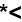
\includegraphics{Comment_line}] Insère une ligne de commentaire à la position actuelle du curseur. Ctrl-Alt-L
\begin{lstlisting}
void MyClass::Foo(bool bar)
{
    fooBar(bar); /**<  */
}
\end{lstlisting}

\item[
\includegraphics{Html}] Affiche la documentation HTML générée. Ctrl-Alt-H
\item[
\includegraphics{Chm}] Affiche la documentation CHM (Help) générée. Ctrl-Alt-C
\item[
\includegraphics{Configure}] Ouvre les préférences de DoxyBlocks. Ctrl-Alt-P
\end{description}

Doxyblocks ne peut travailler que si doxygen est installé sur votre système. Vous avez besoin au moins des exécutables de doxygen et de doxywizard (disponibles dans la distribution officielle de doxygen sur \url{http://www.doxygen.nl/}). En option, vous pouvez avoir l'exécutable "dot" du package graphviz (voir \url{https://graphviz.gitlab.io/}. Sous Windows, le compilateur d'aide (hhc) peut également être utilisé les fichiers de type chm.

\genterm{Notes}
\begin{description}
\item Dans les préférences, vous avez une case à cocher qui autorise ou pas DoxyBlocks à \textbf{écraser le fichier doxyfile}. Par défaut, si un doxyfile existe déjà il ne sera pas écrasé pour protéger de divers changements qui auraient pu être faits en dehors de DoxyBlocks. Néanmoins ce comportement empèche aux changements faits par DoxyBlocks lui-même d'être écrits dans le doxyfile existant.
\item Si un champ de texte des "Préférences" est vide, DoxyBlocks assumera que l'exécutable correspondant est disponible quelquepart via votre variable d'environnement path. Vous pouvez utiliser des macros telles que \$(CODEBLOCKS) dans votre path et elles seront automatiquement étendues.
\item [OUTPUT\_DIRECTORY] Utilisé pour spécifier le chemin de base (relatif ou absolu) ou sera enregistrée la documentation générée. Si un chemin relatif est entré, il sera en relatif par rapport à l'emplacement d'où doxygen a été lancé. Si laissé en blanc, c'est le répertoire courant qui sera utilisé. Doxyblocks utilisera le nom de chemin entré ici pour créer un répertoire relatif au \codeline{<rep. projet>}. Ceci vout permet de créer des répertoire doxygen différents pour des projets inclus dans un même répertoire, ou simplement utiliser un nom de répertoire différent. Si le champ est laissé en blanc, les documents seront créés dans "\codeline{<rep. projet>/doxygen}". Entrer les noms de répertoires sans points, ni séparateurs de tête, ni nom de volume, etc. DoxyBlocks effectue la validation sur le nom de chemin et supprime les caractères en trop.
\begin{verbatim}
Exemples:
[blanc]           -> <répertoire projet>/doxygen.
"docs"            -> <répertoire projet>/docs.
"docs/sub1/sub2"  -> <répertoire projet>/docs/sub1/sub2.
"doxygen/docs"    -> <répertoire projet>/doxygen/docs.
\end{verbatim}
\item [OUTPUT\_LANGUAGE]  Utilisé pour spécifier dans quelle langue sera générée la documentation par doxygen. Doxygen utilisera cette information pour générer toutes les sorties constantes dans la langue adéquate. La langue par défaut est l'anglais. D'autres langues sont supportées. 
\item D'autres informations dans les fichiers d'aide de doxygen
\end{description}
\end{DOXYBLOCKS}

\begin{EDITORTWEAKS}
\section{Extension Editor Tweaks}\label{sec:editor_tweaks}

Le plugin EditorTweaks (modifications d'édition) apporte plusieurs fonctionnalités différentes. Sur une base de travail fichier à fichier, il contrôle :

\begin{itemize}[noitemsep]
\item le repliement de mots ;
\item la numérotation des lignes ;
\item l'interprétation de la touche tab (caractère de tabulation ou espaces) ;
\item le nombre de caractères espace remplaçant la touche tab ;
\item les caractères de fin de ligne (carriage-return + linefeed; carriage-return; linefeed) ;
\item la visualisation des caractères de fin de ligne ;
\item sur demande, la suppression des espaces blancs en fin de ligne ;
\item sur demande, la synchronisation des caractères de fin de ligne ;
\item la suppression de la touche d'insertion.
\end{itemize}

Depuis la fusion avec le plugin "Aligner", il peut rendre des sections de code plus lisibles en les alignant sur un caractère spécifique.\newline
Par exemple, aligner sur le caractère "=" dans :

\begin{lstlisting}
int var = 1;
int longVarName = 2;
int foobar = 3;
\end{lstlisting}

se traduira par :

\begin{lstlisting}
int var         = 1;
int longVarName = 2;
int foobar      = 3;
\end{lstlisting}

\end{EDITORTWEAKS}

\begin{ENVVAR}
\section{Extension Variables d'Environnement}\label{sec:EnvVar_Plugin}

D'après le wiki de \codeblocks. Voir aussi la \pxref{sec:EnvVars_Cfg}.

L'extension \textbf{Éditeur de variables d'environnement} permet de définir des variables d'environnement du système dans le cadre de \codeblocks.\newline
L'utilisateur peut avoir plusieurs ensembles qui contiennent 1..n variables d'environnement.\newline
L'utilisateur peut passer d'un ensemble à l'autre via la boîte de dialogue de configuration des variables d'environnement.\newline
En outre, l'extension EnvVars apporte une option aux projets (dans la configuration du projet) pour appliquer un ensemble EnvVar particulier à activer (et à utiliser pendant la compilation).

La boîte de dialogue permettant de modifier les ensembles se trouve dans \menu{Paramètres,Environnement,Variables d'environnement}.\newline
La boîte de dialogue permettant de choisir l'ensemble actif pour le projet en cours se trouve dans \menu{Projet,Propriétés,Options EnvVar}.\newline

\textbf{Script binding}

Cette extension apporte sa fonctionnalité via un "squirrel binding" : 

{\footnotesize
\begin{longtable}{|l|l|l|l|}\hline
\textbf{Valeur de retour}&\textbf{Nom}      &\textbf{Arguments}     &\textbf{Remarques}                     \\ \hline
\endhead    % Pour répéter la ligne de titre si besoin
wxArrayString   &EnvvarGetEnvvarSetNames    &                       &Retourne tous les ensembles            \\
                &                           &                       &envvar disponibles                     \\ \hline
wxString        &EnvvarGetActiveSetName     &                       &Retourne le nom de l'ensemble          \\
                &                           &                       &actif courant                          \\
                &                           &                       &(depuis config, /active\_set)          \\ \hline
wxArrayString   &EnvVarGetEnvvarsBySetPath  &const wxString         &Retourne les envvars d'un              \\
                &                           &set\_name              &chemin d'ensembles envvars             \\
                &                           &                       &dans la config                         \\ \hline
bool            &EnvvarSetExists            &const wxString         &Vérifie si un ensemble d'envvars       \\
                &                           &set\_name              &existe effectivement dans la config    \\ \hline
bool            &EnvvarSetApply             &const wxString\&       &Applique un ensemble envvar            \\
                &                           &set\_name,             &spécifique de la config                \\
                &                           &bool even\_if\_active  &(sans interaction de l'IU)             \\ \hline
void            &EnvvarSetDiscard           &const wxString         &Ignore un ensemble envvar              \\
                &                           &                       &spécifique de la config                \\
                &                           &                       &(sans interaction de l'IU)             \\ \hline
bool            &EnvvarApply                &const wxString key,    &Applique un envvar spécifique          \\
                &                           &const wxString value   &                                       \\ \hline
bool            &EnvvarDiscard              &const wxString key     &Ignore un envvar                       \\ \hline
\caption{Squirrel binding}
\end{longtable}
\par}

\textbf{NOTE} : Les arguments "value" sont automatiquement générés à partir des macros. Vous n'avez pas besoin d'appeler ReplaceMacros() sur ceux-ci.

Beaucoup d'autres fonctions de script sont disponibles. Regardez dans \url{https://wiki.codeblocks.org/index.php/Scripting_commands}

\textbf{Exemple}

Dans les fenêtres des étapes de post ou pré-génération :
\begin{lstlisting}
[[EnvvarApply(_("test"),_("testValue"));]]
echo %test%
\end{lstlisting}


\end{ENVVAR}

\begin{FILEMANAGER}
\section{Extensions FileManager et PowerShell}\label{sec:file_explorer}

L'explorateur de fichiers \pxref{fig:file_explorer} est inclus dans l'extension FileManager, et se trouve dans l'onglet  \samp{Fichiers}. L'aspect de File Explorer est montré à la \pxref{fig:file_explorer}.

En haut vous trouverez le champ d'entrée du chemin. En cliquant sur le bouton à l'extrémité de ce champ, la flèche vers le bas listera un historique des entrées précédentes dans lesquelles on peut naviguer à l'aide d'une barre de défilement. La flèche vers le haut à droite du champ déplace d'un cran vers le haut dans la structure des répertoires.

Dans le champ \samp{Joker} vous pouvez entrer un filtre de visualisation pour l'affichage des fichiers. En laissant vide ce champ ou en y entrant \codeline{*} vous afficherez tous les fichiers. En y entrant \codeline{*.c;*.h} par exemple, vous n'afficherez que les fichiers sources en C et les fichiers d'en-têtes (headers). Ouvrir la flèche du bas, affiche de nouveau la liste des dernières entrées.

\figures[hbt!]{file_explorer}{Le gestionnaire de fichiers}

Appuyer sur la touche Maj tout en cliquant, sélectionne un groupe de fichiers ou de répertoires, alors qu'appuyer sur la touche Ctrl tout en cliquant sélectionne des fichiers multiples ou des répertoires séparés.

Les opérations suivantes peuvent être obtenues via le menu de contexte si un ou plusieurs répertoires ont été sélectionnés dans l'Explorateur de Fichiers :

\begin{description}
\item[Make Root] défini le répertoire courant comme répertoire de base.
\item[Ajouter aux favoris] configure un marqueur pour ce répertoire et l'enregistre dans les favoris. Cette fonction permet de naviguer rapidement entre des répertoires fréquemment utilisés ou encore sur des disques réseau.
\item[Nouveau Fichier] crée un nouveau fichier dans le répertoire sélectionné.
\item[Nouveau Répertoire] crée un nouveau sous répertoire dans le répertoire sélectionné.
\end{description}

Les opérations suivantes peuvent être obtenues via le menu de contexte si un ou plusieurs fichiers ou même un ou plusieurs répertoires ont été sélectionnés dans l'Explorateur de Fichiers :

\begin{description}
\item[Dupliquer] copie un fichier/répertoire et le renomme.
\item[Copier vers] ouvre une boîte de dialogue pour entrer un répertoire cible dans lequel on copiera les fichiers/répertoires.
\item[Déplacer vers] déplace la sélection vers un autre endroit.
\item[Supprimer] supprime les fichiers/répertoires sélectionnés.
\item[Afficher les fichiers masqués] active/désactive l'affichage des fichiers systèmes masqués. Si activé, le menu est coché par un marqueur.
\item[Actualiser] actualise l'affichage de l'arborescence des répertoires.
\end{description}

Les opérations suivantes peuvent être obtenues via le menu de contexte si un ou plusieurs fichiers ont été sélectionnés dans l'Explorateur de Fichiers :

\begin{description}
\item[Ouvrir dans l'éditeur CB] ouvre le fichier sélectionné dans l'éditeur de \codeblocks.
\item[Renommer] renomme le fichier sélectionné.
\item[Ajouter au projet actif] ajoute le(s) fichier(s) au projet actif.
\end{description}

\hint{Les fichiers/répertoires sélectionnés dans l'explorateur de fichiers peuvent être accédés dans l'extension PowerShell à l'aide de la variable \codeline{mpaths}.}

On peut spécifier via la commande de menu \menu{Paramètres,Environnement,PowerShell} des fonctions utilisateur. Dans le masque de PowerShell, une nouvelle fonction qui peut être nommée aléatoirement, est créée via le bouton \samp{Nouveau}. Dans le champ \samp{ShellCommand Executable}, le programme exécutable est spécifié, et dans le champ en bas de la fenêtre, des paramètres additionnels peuvent être passés au programme.
En cliquant sur la fonction dans le menu de contexte ou dans le menu de PowerShell, la fonction s'exécute et traite les fichiers/répertoires sélectionnés. La sortie est redirigée vers une fenêtre de Shell séparée.

Par exemple une entrée de menu a été créée dans \menu{PowerShell,SVN} et dans le menu de contexte en tant que \samp{SVN}. Dans ce contexte \codeline{$file} signifie le fichier sélectionné dans l'explorateur de fichiers, \codeline{$mpath} les fichiers ou répertoires sélectionnés (voir \pxref{sec:builtin_variables}).

\begin{lstlisting}
 Ajouter;$interpreter add $mpaths;;;
\end{lstlisting}

Celle-ci et toutes les commandes suivantes créeront un sous-menu, dans ce cas \menu{Extensions,SVN,Ajouter}. Le menu de contexte est étendu de même. Cliquez sur la commande du menu de contexte pour faire exécuter la commande SVN \codeline{add} sur les fichiers/répertoires sélectionnés.

TortoiseSVN est un programme SVN très répandu qui s'intègre dans l'explorateur. Le programme \file{TortoiseProc.exe} de TortoiseSVN peut être démarré en ligne de commande et affiche une boîte de dialogue pour y entrer les données de l'utilisateur. Ainsi vous pouvez lancer des commandes, disponibles en tant que menus de contexte dans l'explorateur, également en ligne de commande. Vous pouvez donc l'intégrer en tant qu'extension du Shell dans  \codeblocks. Par exemple, la commande

\begin{lstlisting}
TortoiseProc.exe /command:diff /path:$file
\end{lstlisting}

affichera les différences entre un fichier sélectionné dans l'explorateur de \codeblocks et celui de la base de SVN. Voir \pxref{fig:interpreter} comment intégrer cette commande.
\hint{Pour les fichiers qui sont sous le contrôle de SVN l'explorateur de fichier affiche des icônes superposées qui s'activent via le menu \menu{Vue,SVN Decorators}.}

\screenshot{interpreter}{Ajout d'une extension Shell au menu de contexte}

\genterm{Exemple}

Vous pouvez utiliser l'explorateur de fichiers pour afficher les différences sur des fichiers ou des répertoires. Suivez les étapes suivantes :

\begin{enumerate}
\item Ajoutez le nom via le menu \menu{Paramètres,Environnement,PowerShell}. C'est affiché comme une entrée par l'interpréteur de menu et le menu de contexte.
\item Sélectionnez le chemin absolu de l'exécutable Diff (notamment kdiff3). Le programme est accédé avec la variable \codeline{$interpreter}.
\item Ajoutez les paramètres de l'interpréteur
\begin{lstlisting}
Diff;$interpreter $mpaths;;;
\end{lstlisting}
\end{enumerate}

Cette commande sera exécutée en utilisant les fichiers ou répertoires sélectionnés en tant que paramètres. La sélection peut être accédée via la variable \codeline{$mpaths}. Ceci est une façon commode de différentier des fichiers ou des répertoires.

\hint{L'extension supporte l'utilisation des variables de \codeblocks dans l'extension du Shell.}

% Actions string format: Name;Command;[W|C];WorkDir;EnvVarSet
% (the last two ; delimit settings for the working directory and (not implemented) environment variable set)
%
\begin{description}
\item[\$interpreter] Appelle cet exécutable.
\item[\$fname] Nom du fichier sans son extension.
\item[\$fext] Extension du fichier sélectionné.
\item[\$file] Nom du fichier.
\item[\$relfile] Nom du fichier sans l'information de chemin.
\item[\$dir] Nom du répertoire sélectionné.
\item[\$reldir] Nom du répertoire sans l'information de chemin.
\item[\$path] Chemin absolu.
\item[\$relpath] Chemin relatif du fichier ou du répertoire
\item[\$mpaths] Liste des fichiers et répertoires sélectionnés actuellement
\item[\$inputstr\{ msg \}] Chaîne de caractères qui est entrée dans une fenêtre de message.
\item[\$parentdir] Répertoire Parent (../).
\end{description}

\hint{Les entrées de l'extension Shell sont également disponibles en tant que menus de contexte dans l'éditeur de \codeblocks.}
%Support for personalities.
%Bsp:
%%View;latex $fname.$fext;W;$parentdir
%
%\subsection{Support for Version Control Systems}
%
%Context menu \menu{View, SVN Decorators}
% Run the processes using option 'W' in the action string (to run an interpreter in the cbconsole runnner use 'C' in the action string). for example a python run action string to run a script in a dockable window tab might look like this:
%
% \begin{lstlisting}
% 'Run;$interpeter -u $file;W;;'
% \end{lstlisting}
%
% Command line variables:
% \begin{lstlisting}
% $interpreter, $file, $dir, $path, $mpaths
% Working directory variables: $dir, $parentdir
% \end{lstlisting}
%


\end{FILEMANAGER}

\begin{HEXEDITOR}
\section{Éditeur Hexadécimal}\label{sec:hexeditor}

Comment ouvrir un fichier via HexEditor dans \codeblocks.

\begin{enumerate}
\item \menu{Fichier, Ouvrir avec HexEditor}
\item Menu contextuel du navigateur de projet (\menu{Ouvrir avec,Hex editor}
\item Sélectionnez l'onglet Fichier dans le panneau de gestion. En sélectionnant un fichier dans le Gestionnaire de fichiers et en exécutant le menu contextuel \menu{Ouvrir avec Hex Editor}, le fichier s'ouvre dans HexEditor.
\end{enumerate}

Répartition des fenêtres :

À gauche la Vue de HexEditor et à droite l'affichage sous forme de chaînes de caractères

\textbf{Ligne du haut :}
Position actuelle (valeur en décimal/hex) et pourcentage (rapport entre la position actuelle du curseur et le fichier complet).

\textbf{Boutons :}

\textbf{Fonctions de recherche}

\textit{Bouton Aller à :}
Sauter à une position absolue. Format décimal ou hexadécimal. Saut relatif vers l'avant ou vers l'arrière en spécifiant le signe.

\textit{Chercher :}
 Recherchez des motifs hexadécimaux dans la vue HexEditor ou des chaînes de caractères dans la vue d'aperçu de fichier.

\textit{Configuration du nombre de colonnes :}
Exactement, Multiple de, Puissance de

\textit{Mode d'affichage :}
Hexa, Binaire

\textit{Octets :}
Sélectionnez le nombre d'octets à afficher par colonne.

\textit{Choix d'Endianess :}
BE: Big Endian
LE: Little Endian

\textit{Valeur Prévisualisée :}
Ajoute une vue supplémentaire dans HexEditor. Pour une valeur sélectionnée dans HexEditor, la valeur est également affichée sous forme de Word, Dword, Float, Double.

\textit{Entrée d'expression :}
Permet d'effectuer une opération arithmétique sur une valeur dans HexEditor. Le résultat de l'opération est affiché dans la marge de droite.

\textit{Calc :}
Testeur d'Expression

\textit{Édition d'un fichier dans HexEditor :}

Commandes d'historique Annuler (Undo) et Refaire (Redo).

Autre exemple, Déplacer le curseur dans la vue des chaînes de caractères :
Insérer des espaces avec la touche Insérer.
Supprimer des caractères en appuyant sur la touche Suppr.

En saisissant un texte, le contenu existant est écrasé sous la forme d'une chaîne de caractères.

En saisissant des chiffres dans la vue d'HexEditor, les valeurs sont écrasées et l'aperçu est mis à jour.


\end{HEXEDITOR}

\begin{INCREMENTALSEARCH}
\section{Recherche Incrémentale}

Pour obtenir une recherche efficace dans des fichiers ouverts, \codeblocks fourni ce qu'on nomme une recherche incrémentale. Cette méthode de recherche s'initialise, pour un fichier ouvert, via le menu \menu{Rechercher,Recherche Incrémentale} ou par le raccourci clavier Ctrl-I. L'entrée active passe alors automatiquement à la configuration du masque de recherche dans la barre d’outils correspondante. Dès que vous commencez à entrer des termes de recherche, le fond du masque de recherche s'ajuste en fonction des occurrences des termes. Si un accord est trouvé dans l'éditeur actif, la position respective est marquée en couleur. Par défaut l'accord courant est surligné en vert. Cette configuration peut être changée dans \menu{Paramètres, Éditeur, Recherche Incrémentale} (voir \pxref{fig:incremental_search_settings}). En appuyant sur la touche Entrée la recherche saute à l'occurrence suivante de la chaîne de texte recherchée à l'intérieur du fichier. Avec Maj-Entrée, c'est l'occurrence précédente qui est sélectionnée. Cette fonctionnalité n'est pas supportée par Scintilla si la recherche incrémentale utilise des expressions régulières.

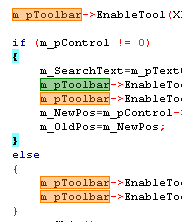
\includegraphics{incremental_search_example}

Si la chaîne de caractère recherchée ne peut pas être trouvée dans le fichier courant, afin d'indiquer que c'est ce qui se passe, le fond du masque de recherche est affiché en rouge.

\screenshot{incremental_search_settings}{Paramètres pour la Recherche Incrémentale}

\begin{description}
\item[ESC] Quitte le module de Recherche Incrémentale.
\item[ALT-Suppr] Efface l'entrée du champ de recherche incrémentale.
\end{description}

Les icônes de la barre d’outils de Recherche Incrémentale ont les significations suivantes :

\begin{description}
\item[
\includegraphics{incremental_search_clear}] Suppression du texte dans le masque de recherche de la barre d'outils de Recherche Incrémentale.
\item[
\includegraphics{incremental_search_previous},
\includegraphics{incremental_search_next}] Navigation dans les occurrences de chaîne recherchée.
\item[
\includegraphics{incremental_search_highlight}] En cliquant sur ce bouton ce sont toutes les occurrences de la chaîne recherchée qui sont surlignées en couleur, pas seulement la première.
\item[
\includegraphics{incremental_search_selected}] Activer cette option réduit le champ de recherche au passage de texte marqué dans l'éditeur.
\item[
\includegraphics{incremental_search_matchcase}] Cette option signifie que la recherche sera sensible à la casse (respect des majuscules et minuscules).
\item[
\includegraphics{incremental_search_regex}] Valider les expressions régulières dans le champ d'entrée de la recherche incrémentale.
\end{description}

\hint{Le paramétrage standard de cette barre d'outil peut être configuré dans \menu{Paramètres,Éditeur,Recherche Incrémentale}.}

%\screenshot{incremental_search_settings}{Paramètres pour la Recherche Incrémentale}

\end{INCREMENTALSEARCH}

\begin{NASSISHNEIDERMAN}
\section{Extension NassiShneiderman}\label{sec:nassishneiderman}

L'extension NassiShneiderman permet de créer des diagrammes de Nassi Shneiderman depuis \codeblocks (\cite{url:nassi}). 

\subsection{Création d'un diagramme}

Vous avez deux possibilités pour créer un diagramme.

\begin{enumerate}
\item Pour créer un diagramme vide, sélectionnez les options de menu \menu{Fichier,Nouveau,Diagramme de Nassi Shneiderman}.
\item La deuxième option consiste à créer un diagramme depuis le code source C/C++. 
\end{enumerate}

Dans une fenêtre de l'éditeur, sélectionnez une partie de code pour en créer un diagramme. Par exemple le corps d'une fonction/méthode depuis l'accolade ouvrante jusqu'à l'accolade fermante. Puis, via un clic droit sur la sélection, choisissez \menu{Nassi Shneiderman,Créer un diagramme} (voir \pxref{fig:NassiShneidermanCreate1}). 

\screenshot{NassiShneidermanCreate1}{NassiShneiderman Création}

Vous devriez obtenir un nouveau diagramme (voir \pxref{fig:NassiShneidermanCreate2}).

\screenshot{NassiShneidermanCreate2}{NassiShneiderman Exemple de Diagramme}

L'analyseur a quelques limitations:

\begin{itemize}
\item Des commentaires ne peuvent pas être placés en fin de branche.
\item Depuis la définition d'une fonction, on ne peut analyser que le corps de la fonction, pas la déclaration.
\item Bien sûr, vous en trouverez bien d'autres... 
\end{itemize}

\subsection{Édition de structogrammes}
\subsubsection{Que faire avec un diagramme ?}

Vous pouvez faire plein de choses avec un structogramme :

\begin{enumerate}
\item L'enregistrer pour l'utiliser plus tard. On peut l'enregistrer via \menu{Fichier,Enregistrer le fichier} ou \menu{Fichier,Enregistrer le fichier sous...}.
\item On peut l'exporter dans différents formats \menu{Fichier,Exporter}
    \begin{itemize}
    \item "Exporter la source..." pour l'enregistrer comme fichier source en C.
    \item "StrukTeX" pour l'utiliser dans une documentation sous LaTeX.
    \item "PNG" ou "PS" et éventuellement "SVG" pour obtenir le diagramme dans un format image connu de nombreux autres outils.
    \end{itemize}        
\item Insérer directement le code dans l'éditeur : Ouvrir ou créer un diagramme. De retour dans la fenêtre d'édition, faites un clic droit et choisissez \menu{Nassi Shneiderman,insérer en xy} (Vous obtenez ici une liste de tous les diagrammes ouverts).
\item Glisser/Déposer le diagramme (ou une partie) dans d'autres outils. Par exemple vers OpenOffice Writer afin d'y insérer une image dans votre documentation.
\end{enumerate}

Si le diagramme choisi comporte une sélection, l'exportation ou la génération de code ne portera que sur cette partie de diagramme. 

\subsubsection{Extensions}

L'extension NassiShneiderman supporte quelques extensions des diagrammes de Nassi-Shneiderman : 

\begin{itemize}
\item séparation d'une brique spécifique avec la "flèche droite"
\item continuer sur une brique spécifique avec la "flèche gauche"
\item Pour être en mesure de créer des diagrammes avec des instructions c/c++ "switch", la sélection ne doit pas être implicitement interrompue avant un "case". Les différents "cases" sont alignés verticalement. Support de C et C++.
\end{itemize}


\end{NASSISHNEIDERMAN}

\begin{LIBFINDER}
\section{LibFinder}\label{sec:lib_finder}

Si vous voulez utilisez des librairies dans votre application, vous devez configurer votre projet pour cela. Un tel processus de configuration peut être difficile et ennuyeux car chaque librairie peut utiliser un schéma d'options particulier. Un autre problème est que cette configuration diffère entre les plates-formes ce qui résulte en des incompatibilités entre des projets Unix et Windows.

LibFinder propose deux fonctionnalités majeures :

\begin{itemize}
\item Recherche des librairies installées sur votre système
\item Inclure les librairies dans votre projet en seulement quelques clics en rendant le projet indépendant de la plate-forme
\end{itemize}

\subsection{Recherche de librairies}

La recherche des librairies est disponible via le menu \menu{Extensions,Library finder}. Son but est de détecter les librairies installées sur votre système et d'enregistrer les résultats dans la base de données de LibFinder (notez que ces résultats ne sont pas écrits dans les fichiers projets de \codeblocks). La recherche commence par un dialogue où vous pouvez fournir un ensemble de répertoires où sont installées les librairies. LibFinder les analysera de façon récursive aussi, si vous ne savez pas trop où elles sont, vous pouvez sélectionner des répertoires génériques. Vous pouvez même entrer le disque complet -- dans ce cas-là, le processus de recherche prendra plus de temps mais il détectera davantage de librairies (voir \pxref{fig:list_of_directories}).

\screenshot{list_of_directories}{Liste de répertoires}

Quand LibFinder est à la recherche de librairies, il utilise des règles spéciales pour détecter leur présence. Chaque ensemble de règle est situé dans un fichier xml. Actuellement LibFinder peut rechercher wxWidgets 2.6/2.8, \codeblocks SDK et GLFW -- la liste sera étendue dans le futur.

\hint{Pour obtenir davantage de détails sur comment ajouter un support de librairie dans LibFinder, lisez dans les sources de \codeblocks \file{src/plugins/contrib/lib\_finder/lib\_finder/readme.txt}.}

Après avoir terminé l'analyse, LibFinder affiche les résultats (voir \pxref{fig:search_results}).

\screenshot{search_results}{Résultats de recherche}

Dans la liste, vous cochez les librairies qui doivent être enregistrées dans la base de données de LibFinder. Notez que chaque librairie peut avoir plus d'une configuration valide et les paramétrages ajoutés en premier sont plutôt destinés à être utilisés lors de la génération de projets.

Au-dessous de la liste, vous pouvez sélectionner ce qu'il faut faire avec les résultats des analyses précédentes :

\begin{description}
\item[Ne pas effacer les résultats précédents] Cette option travaille comme une mise à jour des résultats existants -- Cela ajoute les nouveaux et met à jour ceux qui existent déjà. Cette option n'est pas recommandée.
\item[Seconde option (Effacer les résultats précédents des librairies sélectionnées)] effacera tous les résultats des recherches précédentes des librairies sélectionnées avant d'ajouter les nouveaux résultats. C'est l'option recommandée.
\item[Effacer toutes les configurations précédentes des librairies] quand vous sélectionnez cette option, la base de données de LibFinder sera effacée avant d'y ajouter les nouveaux résultats. C'est utile quand vous voulez nettoyer une base de données LibFinder contenant des résultats invalides.
\end{description}

Une autre option de ce dialogue est \menu{Configurer les Variables Globales}. Quand vous cochez cette option, LibFinder essaiera de configurer des Variables Globales qui sont aussi utilisées pour aider à  traiter les librairies.

Si vous avez pkg-config d’installé sur votre système (C'est installé automatiquement sur la plupart des versions de systèmes linux) LibFinder proposera des librairies venant de cet outil. Il n'est pas nécessaire de faire une analyse spécifique pour celles-ci -- elles seront automatiquement chargées au démarrage de \codeblocks.

\subsection{Inclure des librairies dans les projets}

LibFinder ajoute un onglet supplémentaire dans les propriétés d'un projet \menu{Librairies} -- Cet onglet montre les librairies utilisées dans le projet ainsi que celles connues de LibFinder. Pour ajouter une librairie dans votre projet, sélectionnez là dans le panneau de droite et cliquez sur le bouton $<$. Pour enlever une librairie d'un projet, sélectionnez la dans le panneau de gauche et cliquez sur le bouton $>$ (voir \pxref{fig:project_configuration}).

\screenshot{project_configuration}{Configuration de projet}

Vous pouvez filtrer les librairies connues de LibFinder en fournissant un filtre de recherche. La case à cocher \menu{Afficher comme un arbre}  permet de basculer antre des vues sans catégories et des vues avec catégories.

Si vous voulez ajouter une librairie qui n'est pas disponible dans la base de données de LibFinder, vous pouvez utiliser le champ \menu{Librairie inconnue}. Notez que vous devriez entrer le "library's shortcode" (nom court, qui habituellement correspond au nom de variable globale) ou le nom de librairie dans pkg-config. Vous trouverez une liste de noms courts suggérés dans le Wiki de \codeblocks dans \href{http://wiki.codeblocks.org/index.php?title=Recommended_global_variables}{Global Variables}. L'usage de cette option n'est recommandé que lorsqu'on prépare un projet qui doit être généré sur d'autres machines où ce type de librairie existe et y est correctement détectée par LibFinder. Vous pouvez accéder à une variable globale dans \codeblocks comme :

\begin{lstlisting}
$(#GLOBAL_VAR_NAME.include)
\end{lstlisting}

Cocher l'option \menu{Ne pas configurer automatiquement} indiquera à LibFinder qu'il ne devrait pas ajouter automatiquement les librairies lors de la compilation. Dans ce cas, LibFinder peut s'invoquer depuis un script de génération. Un exemple d'un tel script est généré et ajouté au projet en appuyant sur  \menu{Ajouter un script de génération manuel}.

\subsection{Utilisation de LibFinder dans des projets générés par des assistants}

Les assistants vont créer des projets qui n'utilisent pas LibFinder. Pour les intégrer avec cette extension, vous devrez mettre à jour manuellement les options de génération du projet. Ceci est facilement obtenu en enlevant tous les paramétrages spécifiques aux librairies et en ajoutant les librairies au travers de l'onglet \menu{Librairies} dans les propriétés du projet.

De tels projets deviennent indépendants des plates-formes. Tant que les librairies utilisées sont dans la base de données de LibFinder, les options de génération du projet seront automatiquement mises à jour pour coïncider avec les paramétrages de librairie propres aux plates-formes.




\end{LIBFINDER}

\begin{SPELLCHECKER}
\section{Extension SpellChecker}\label{sec:spell_checker}

Une extension pour vérifier l'orthographe de chaînes de caractères et de commentaires.

\subsection{Introduction}
Une extension pour vérifier l'orthographe de chaînes de caractères et de commentaires. L'orthographe est vérifiée au cours de la frappe. De plus un thésaurus est fourni. Les deux peuvent être accédés sur demande en sélectionnant le mot en question, puis choisir entre le correcteur... ou le Thesaurus... depuis le menu d'Édition (l'opération peut être affectée à une touche d'accès rapide via le plugin Raccourcis Clavier). Le menu de contexte (clic droit sur le mot) permet d'accéder aux suggestions d'orthographe. 

\subsection{Configuration}

La configuration est dans le menu \menu{Paramêtres,Éditeur}. L'option "spell check" est à peu près à mi-chemin vers le bas de la liste de gauche.

\screenshot{ConfigureSpellChecker}{Configuration de SpellChecker}

La signification des différents contrôles est la suivante : 
\begin{description}
\item[Activer spell checker en-ligne] Active ou désactive spell checker.
\item[Langue] La langue utilisée pour la vérification orthographique et le thésaurus est sélectionnée en choisissant un dictionnaire. On peut aussi le changer dans la barre d'état.
\item[Configuration des chemins, Dictionnaires] Le plugin cherche les fichiers dictionnaires via ce chemin.
\item[Configuration des chemins, Thésaurus] Le plugin cherche les fichiers thésaurus via ce chemin.
\item[Configuration des chemins, Bitmaps] (Optionnel) Le plugin cherche, via ce chemin, les drapeaux à afficher dans la barre d'état.
\end{description}

\hint{Vous pouvez utiliser des Macros dans les trois configurations de chemins, comme par ex. \$(CODEBLOCKS)/share/codeblocks/SpellChecker. Voir Expansion de Variables pour plus de détails. Ceci est pratique si vous utilisez une version portable de \codeblocks.}

\subsection{Dictionnaires}

SpellChecker utilise une librairie nommée hunspell. Hunspell est le correcteur orthographique de OpenOffice.org, Mozilla Firefox et d'autres projets. Les dictionnaires disponibles pour ces applications sont compatibles avec ce plugin.

Open Office fourni toute une collection de dictionnaires pour plusieurs langues et dialectes à télécharger. Les extensions de OOo 3.x (*.oxt) sont des archives compressés qui peuvent être ouvertes avec votre logiciel d'archives préféré (par exemple 7-Zip ou File Roller). Copiez le fichier .aff et le fichier .dic dans le répertoire configuré dans 'Configuration des chemins, Dictionnaires' (voir ci-dessus).

Si vous êtes sous Linux vous avez sans doute déjà des dictionnaires compatibles d'installés. Regardez dans /usr/share/hunspell ou plutôt mon choix dans /usr/share/myspell/dicts. La raison pour laquelle j'aime les fichiers myspell est qu'ils incluent d'office les fichiers thésaurus qui sont correctement nommés pour travailler avec l'extension, et tout est placé au même endroit. Ne copiez pas ces fichiers. Pointez seulement spell checker vers l'endroit où ils se trouvent déjà.

Je sais que sous Windows, Firefox et Thunderbird installent aussi des fichiers dictionnaires compatibles. On peut les trouver dans... \file{C:\osp Program Files\osp Mozilla Firefox\osp dictionaries} ou \file{C:\osp Program Files\osp Mozilla Thunderbird\osp dictionaries}. De plus, OpenOffice.org et LibreOffice installent aussi des fichiers dictionnaires dans\newline
 \file{C:\osp Program Files\osp (Open/Libre)Office\osp share\osp extensions\osp dict-*}.

Le navigateur Google Chrome installe aussi des dictionnaires, mais ils sont au format .bdic et le plugin de correction orthographique de \codeblocks ne peut pas travailler avec ces fichiers.

\subsection{Fichiers Thésaurus}

Les fichiers de thésaurus sont aussi disponibles sur OOo, comme les dictionnaires. Copiez les fichiers de thésaurus (th\_*.dat and th\_*.idx) dans le répertoire configuré dans 'Configuration des chemins, Thésaurus' (voir ci-dessus) puis renommez les pour que leur nom concorde avec celui des dictionnaires mais les faire précéder de "th\_" tout en gardant l'extension telle qu'elle est.

\textbf{Exemple}: Si les fichiers dictionnaires (pour moi, une seule langue) sont "en\_GB.aff" et "en\_GB.dic" les fichiers utilisés pour le thésaurus sont "th\_en\_GB.idx" et "th\_en\_GB.dat".

Sur mon système Linux je trouve les fichiers thésaurus déjà installés dans /usr/share/myspell/dicts et /usr/share/mythes. De même, ne déplacez pas les fichiers. Configurez spell checker pour utiliser directement ces fichiers là où ils sont.

Sous Windows, si soit OpenOffice.org soit LibreOffice est installé, ils incluent souvent les fichiers thésaurus dans \file{C:\osp Program Files\osp (Open/Libre)Office\osp share\osp extensions\osp dict-*}. 

\subsection{Bitmaps (Drapeaux)}

L'image bitmap de la langue sélectionnée est affichée dans la barre d'état. S'il n'y a pas d'image bitmap, c'est le nom de la langue qui s'affiche. L'image bitmap doit être au format PNG Choisissez un drapeau dans famfamfam\_flag\_icons, copiez le dans le répertoire configuré dans 'Configuration des chemins, Bitmaps' (voir ci-dessus) et renommez-le pour que le nom soit conforme à celui du dictionnaire mais gardez l'extension png.

\subsection{Styles à vérifier}

Seul du texte possédant un style spécifique peut être vérifié (par exemple seulement des commentaires et des chaînes de caractères). Les styles sont configurés automatiquement par Scintilla (le composant d'édition de \codeblocks).

Le fichier OnlineSpellChecking.xml contient une liste avec des indices sur les styles à vérifier. Les indices ne sont pas les mêmes en fonction des langages de programmation, et donc, le fichier contient une liste pour chacun des langages de programmation. Pour ajouter des styles, regardez le nom du langage de programmation et les indices dans le fichier correspondant lexer\_*.xml puis ajoutez cette information au fichier OnlineSpellChecking.xml.

Par exemple, pour vérifier l'orthographe dans des scripts de commande bash (fichiers *.sh), ajoutez la ligne : 

\codeline{<Language name="Bash" index="2,5,6" />}

\end{SPELLCHECKER}

\begin{SRCEXPORTER}
\section{Exporter du code Source}\label{sec:src_exporter}

Il est souvent nécessaire de transférer du code source vers d'autres applications ou vers des e-mails. Si le texte est simplement copié, le formatage est perdu, ce qui rend le texte peu clair.
La fonction exporter de \codeblocks est une des solutions dans ce type de situations. Le format requis pour le fichier exporté peut être sélectionné via \menu{Fichier,Exporter}. Le programme adoptera alors le nom de fichier et le répertoire cible en fonction du fichier source ouvert et les proposera pour enregistrer le fichier à exporter. L'extension de fichier appropriée à chaque cas de figure sera déterminée par le type de l'exportation. Les formats suivants sont disponibles :

\begin{description}
\item[html] Un format de type texte qui peut être affiché dans un navigateur web ou dans un traitement de texte.
\item[rtf] Le format Rich Text qui est un format basé sur du texte et qui peut être ouvert dans un traitement de texte comme Word ou OpenOffice.
\item[odt] Le format Open Document Text qui est un format standardisé spécifié par Sun et O'Reilly. Ce format peut être traité par Word, OpenOffice et d'autres traitements de texte.
\item[pdf] Le format Portable Document qui peut être ouvert par des applications comme Acrobat Reader.
\end{description}


\end{SRCEXPORTER}

\begin{SVN}
\section{Support de SVN}\label{sec:svn}

\hint{NdT : Cette extension est traduite ici, mais est obsolète. Vous avez donc de grandes chances de ne plus la trouver dans les versions récentes de \codeblocks.}

Le support du système de contrôle de version SVN est inclus dans l'extension \codeblocks TortoiseSVN. Via le menu \menu{TortoiseSVN,Plugin settings} vous pouvez configurer les commandes svn accessibles dans l'onglet \menu{Integration}.

\begin{description}
\item[Menu intégration] Ajoute une entrée TortoiseSVN dans la barre de menu avec différents paramétrages.
\item[Project manager] Active les commandes TortoiseSVN du menu de contexte de la gestion de projet.
\item[Editor] Active les commandes TortoiseSVN du menu de contexte de l'éditeur.
\end{description}

Dans la configuration de l'extension vous pouvez choisir quelles sont les commandes svn qui sont accessibles dans le menu principal ou le menu de contexte. L'onglet intégration fournit une entrée \menu{Edit main menu} et \menu{Edit popup menu} pour paramétrer ces commandes.

\hint{L'Explorateur de fichiers dans \codeblocks utilise différentes icônes superposées afin d'indiquer l'état de svn. Les commandes de TortoiseSVN sont incluses dans le menu de contexte.}

\end{SVN}

\begin{TODOLIST}
\section{Liste des "à faire"}\label{sec:todo_list}

Dans des projets logiciels complexes, où différents développeurs sont impliqués, il est souvent nécessaire que différentes tâches soient effectuées par plusieurs utilisateurs. Pour cela, \codeblocks possède une Liste des "à faire". Cette liste s'ouvre via \menu{Affichage,Liste des "A faire"}, et contient les tâches à effectuer ensemble, avec leurs priorités, le type et le responsable de la tâche. On peut filtrer la liste par tâches, utilisateurs et/ou fichiers sources. Un tri par colonnes peut être effectué en cliquant sur le titre de la colonne correspondante.

\screenshot{todo_list}{Affichage de la Liste des "A faire"}

\hint{La liste des "à faire" peut être ajoutée à la console de messages. Sélectionnez l'option \samp{Inclure la liste des "A faire" dans le panneau de messages} à l'aide du menu \menu{Paramètres,Environnement}.}

Si les fichiers sources sont ouverts dans \codeblocks, un "à faire" peut être ajouté à la liste via la commande \samp{Ajouter un élément "à faire"} du menu de contexte. Un commentaire est ajouté dans le code sur la ligne sélectionnée.

\begin{lstlisting}
// TODO (user#1#): ajouter un nouveau dialogue pour la prochaine release
\end{lstlisting}

Quand on ajoute un "à faire", une boîte de dialogue apparaît où les paramétrages suivants peuvent être faits (voir \pxref{fig:add_todo}).

\figures[hbt!][width=.5\columnwidth]{add_todo}{Dialogue pour ajouter un "à faire"}

\begin{description}
\item[Utilisateur] Nom de l'utilisateur \var{user} pour le système d'exploitation. Les tâches pour d'autres utilisateurs peuvent également être créées ici. Pour cela, le nom de l'utilisateur correspondant doit être créé par Ajouter un nouvel utilisateur. L'assignation d'un "à faire" est alors faite via une sélection d'entrées pour cet utilisateur.

\hint{Notez que les Utilisateurs ici n'ont rien à voir avec les profils (ou personnalités) utilisés dans \codeblocks.}
\item[Type] Par défaut, le type est TODO (à faire").
\item[Priorité] Dans \codeblocks, l'importance de la tâche peut être exprimée par des priorités (1 - 9).
\item[Position] Ce paramètre spécifie si le commentaire doit être inclus avant, après ou bien à la position exacte du curseur.
\item[Style de commentaire] Une sélection de formats de commentaires (notamment doxygen).
\end{description}

\end{TODOLIST}

\begin{TOOLSPLUS}
\section{Tools+}\label{sec:tools+}

Créer un nouvel outil est assez facile, et cela peut s'effectuer en quelques étapes simples. D'abord ouvrir \menu{Tools(+),Configurer les outils...} pour accéder au dialogue des Outils définis par l'utilisateur.

\screenshot{tools_setup}{Dialogue des Outils définis par l'utilisateur}

\genterm{Nom de l'outil}

C'est le nom qui sera affiché dans le menu déroulant de Tools(+). Il sera aussi affiché comme nom d'onglet pour les Tools+ redirigés vers la fenêtre Outils.

\genterm{Ligne de Commande}

Toute ligne de commande valide, fonction et paramètres, peut être entrée ici. La substitution de variable est également acceptée. La liste suivante contient les variables les plus utiles (voir \pxref{sec:builtin_variables} pour la liste complète).

\begin{description}
\item[\$relfile, \$file] Respectivement, le nom relatif et absolu d'un fichier sélectionné.
\item[\$reldir, \$dir] Respectivement, le nom relatif et absolu d'un répertoire sélectionné.
\item[\$relpath, \$path] Le nom relatif et absolu d'un fichier ou répertoire sélectionné.
\item[\$mpaths] Une liste de fichiers ou de répertoires sélectionnés (seulement des chemins en absolu).
\item[\$fname, \$fext] Le nom sans extension et l'extension sans le nom d'un fichier sélectionné.
\item[\$inputstr\{prompt\}] Demande à l'utilisateur d'entrer une chaîne de texte qui sera substituée dans la ligne de commande.
\item[\$if(condition)\{true clause\}\{false clause\}] Résolution en \codeline{false clause} si la \codeline{condition} est vide, 0, ou fausse; sinon \codeline{true clause}.
\end{description}

\genterm{Types de fichiers}

Les expressions avec un caractère joker (*) séparées par des points virgules vont restreindre le choix par le sous-menu clic droit sur un fichier, répertoire, chemin multiple dans l'arborescence des projets, de l'explorateur de fichiers, ou du panneau d'éditeur à un/des type/s spécifiés. Laisser vide pour traiter tous les types de fichiers/répertoires.

\genterm{Répertoire de Travail}

Le répertoire sur lequel exécuter la commande. Les variables de \codeblocks, les variables de projet, et les variables globales sont disponibles. De même,

\begin{enumerate}
\item Si \codeline{\$dir} est entré dans la ligne de commande, alors \codeline{\$dir} peut aussi être utilisé ici.
\item \codeline{\$parentdir} est disponible pour \codeline{\$relfile}, \codeline{\$file}, \codeline{\$reldir}, \codeline{\$dir}, \codeline{\$relpath}, \codeline{\$path}, \codeline{\$fname}, \codeline{\$fext}, pour l'évaluation du chemin absolu d'un répertoire contenant cet élément.
\end{enumerate}

\genterm{Chemin du Menu Outils}

Contrôle l'emplacement de la commande dans le menu de Tools(+), donnant la possibilité d'ajouter des sous-menus (les niveaux multiples sont autorisés).

\begin{itemize}
  \item Submenu/Tool1
  \item Submenu/Tool2
  \item Tool3
\end{itemize}

Va créer cette structure.

\figures[H][width=.6\columnwidth]{tools_menu_path}{Structure des menus de Tools}

Le nom de la commande sera utilisé si cette entrée est vide. Si le premier caractère est un point, la commande sera cachée.

\genterm{Chemin du Menu de Contexte}

Ceci contrôle l'emplacement de la commande dans le menu clic-droit des Projets et des onglets de fichiers du panneau de Gestion. Les mêmes règles que pour la structure des menu de Tools+ s'appliquent ici.

\figures[H][width=.8\columnwidth]{tools_context_path}{Structure des menus de Contexte}

Notez SVP que la commande n'apparaîtra dans les menus de contexte que si la ligne de commande contient un ou plusieurs des éléments suivants : \codeline{\$relfile}, \codeline{\$file}, \codeline{\$reldir}, \codeline{\$dir}, \codeline{\$relpath}, \codeline{\$path}, \codeline{\$fname}, et \codeline{\$fext}.

\genterm{Sortie vers}

Ceci détermine vers où la sortie de la commande sera redirigée. Le but et la fonction de la commande détermineront ce qui est le mieux à faire.
\genterm{Tools Output Window}
Les outils qui ne requièrent que des résultats de sortie en ligne de commande (et ne demandent pas d'entrées) utilisent généralement cette façon de faire. Le programme sera lancé en mode invisible et toutes les sorties seront redirigées vers l'onglet approprié de la fenêtre de sortie des Outils Tools+. Le texte [DONE/TERMINÉ] sera ajouté en fin d'exécution de l'Outil.

\figures[H][width=.5\columnwidth]{tool_output}{Fenêtre de sortie de l'Outil}

\hint{Si la fenêtre de sortie des Outils Tools+ est ouverte à la clôture de \codeblocks, il se peut que \codeblocks plante.}

\genterm{Console de \codeblocks}
Ceci va permettre de lancer le programme via l'exécutable \file{cb\_console\_runner} (ce même programme qui est lancé après Générer et exécuter). Généralement, c'est utilisé par les outils en ligne de commande pour obtenir des interactions utilisateur avancées, bien que des programmes graphiques puissent aussi être utilisés (notamment si le programme n'est pas stable ou s'il affiche des messages dans la sortie standard). Le "Console runner" mettra la fenêtre en pause (l'empêchant de se fermer), affichera le temps d'exécution, ainsi que le code de sortie quand le programme s'arrêtera.

\genterm{Shell Standard}
C'est la même chose que de placer cette commande dans un script batch ou un script Shell puis de l'exécuter. Le programme s'exécutera quelle que soit la méthode par défaut, et lorsqu'il aura terminé, sa fenêtre se fermera.. Ce paramètre est utile pour exécuter un programme (par exemple un fichier ou un navigateur Web) qui doit rester ouvert après la fermeture de \codeblocks.

\hint{Comme le plugin Tools+ plugin est en cours de développement, quelques fonctionnalités - par exemple Priorité de Menu et Variables d'environnement - peuvent ne pas être disponibles.}

\subsection{Exemple d'Outils Tools+}

\genterm{Ouvrir l'explorateur sur un fichier sélectionné}

\begin{itemize}
\item Windows Explorer
\begin{itemize}
\item Menu Outils Tools+
\begin{verbatim}
explorer /select,"$(PROJECTFILE)"
\end{verbatim}
\item Menu de Contexte
\begin{verbatim}
explorer /select,"$path"
\end{verbatim}
\end{itemize}

\item Dolphin
\begin{itemize}
\item Menu Outils Tools+
\begin{verbatim}
dolphin --select "$(PROJECTFILE)"
\end{verbatim}
\item Menu de Contexte
\begin{verbatim}
dolphin --select "$path"
\end{verbatim}
\end{itemize}

\hint{Les trois commandes suivantes du menu contextuel ne prennent en charge que les dossiers (mais pas les fichiers).}

\item Nautilus
\begin{itemize}
\item Menu Outils Tools+
\begin{verbatim}
nautilus --no-desktop --browser "$(PROJECTDIR)"
\end{verbatim}
\item Menu de Contexte
\begin{verbatim}
nautilus --no-desktop --browser "$dir"
\end{verbatim}
\end{itemize}

\item Thunar
\begin{itemize}
\item Menu Outils Tools+
\begin{verbatim}
thunar "$(PROJECTDIR)"
\end{verbatim}
\item Menu de Contexte
\begin{verbatim}
thunar "$dir"
\end{verbatim}
\end{itemize}

\item PCMan File Manager
\begin{itemize}
\item Menu Outils Tools+
\begin{verbatim}
pcmanfm "$(PROJECTDIR)"
\end{verbatim}
\item Menu de Contexte
\begin{verbatim}
pcmanfm "$dir"
\end{verbatim}
\end{itemize}
\end{itemize}

\genterm{Mise à jour d'un répertoire Subversion}

\begin{itemize}
\item Windows
\begin{itemize}
\item Menus Outils Tools+
\begin{verbatim}
"path_to_svn\bin\svn" update "$inputstr{Directory}"
\end{verbatim}
\item Menu de Contexte
\begin{verbatim}
"path_to_svn\bin\svn" update "$dir"
\end{verbatim}
\end{itemize}

\item Linux
\begin{itemize}
\item Menus Outil Tools+
\begin{verbatim}
svn update "$inputstr{Directory}"
\end{verbatim}
\item Menu de Contexte
\begin{verbatim}
svn update "$dir"
\end{verbatim}
\end{itemize}
\end{itemize}

\genterm{Exporter un makefile}

\hint{Utilisation de l'outil en ligne de commande cbp2make.}\label{sec:tool_cbp2make}

\begin{itemize}
\item Windows
\begin{itemize}
\item Menus Outil Tools+
\begin{verbatim}
"path_to_cbp2make\cbp2make" -in "$(PROJECTFILE)"
\end{verbatim}
\end{itemize}

\item Linux
\begin{itemize}
\item Menus Outil Tools+
\begin{verbatim}
"path_to_cbp2make/cbp2make" -in "$(PROJECTFILE)"
\end{verbatim}
\end{itemize}
\end{itemize}

\genterm{Compresser le projet actif dans une archive}

\begin{itemize}
\item Windows
\begin{itemize}
\item 7z ou zip - Menus Outil Tools+ (sur 1 seule ligne)
\begin{verbatim}
"path_to_7z\7z" a -t$if(zip == $inputstr{7z or zip?}){zip -mm=Deflate
     -mmt=on -mx9 -mfb=128 -mpass=10}{7z -m0=LZMA -mx9 
     -md=64m -mfb=64 -ms=on} -sccUTF-8 "-w$(PROJECTDIR).."
     "$(PROJECTDIR)..\$(PROJECT_NAME)" "$(PROJECTDIR)*"
\end{verbatim}

\item tar.gz ou tar.bz2 - Menus Outil Tools+  (sur 1 seule ligne)
\begin{verbatim}
cmd /c ""path_to_7z\7z" a -ttar -mx0 -sccUTF-8 "-w$(PROJECTDIR).."
      "$(PROJECTDIR)..\$(PROJECT_NAME)" "$(PROJECTDIR)*" && 
      "path_to_7z\7z" a -t$if(gz == $inputstr{gz or bz2?}){gzip -mx9 
      -mfb=128 -mpass=10 -sccUTF-8 "-w$(PROJECTDIR).." 
      "$(PROJECTDIR)..\$(PROJECT_NAME).tar.gz}{bzip2 -mmt=on -mx9 
      -md=900k -mpass=7 -sccUTF-8 "-w$(PROJECTDIR).." 
      "$(PROJECTDIR)..\$(PROJECT_NAME).tar.bz2}"
      "$(PROJECTDIR)..\$(PROJECT_NAME).tar" && 
       cmd /c del "$(PROJECTDIR)..\$(PROJECT_NAME).tar""
\end{verbatim}

\hint{L'interpréteur en ligne de commande de Windows a été invoqué directement ici (\cmdline{cmd /c}), ce qui permet à des commandes multiples de s'enchaîner en une seule ligne. Cependant, cela peut provoquer un échec de l'exécution de la commande dans la console \codeblocks.}

\end{itemize}

\item Linux
\begin{itemize}
\item 7z ou zip - Menu Outils Tools+ (sur 1 seule ligne)
\begin{verbatim}
7z a -t$if(zip == $inputstr{7z or zip?}){zip -mm=Deflate -mmt=on -mx9
    -mfb=128 -mpass=10}{7z -m0=LZMA -mx9 -md=64m -mfb=64 -ms=on}
    -sccUTF-8 "-w$(PROJECTDIR).." "$(PROJECTDIR)../$(PROJECT_NAME)"
    "$(PROJECTDIR)*"
\end{verbatim}
\item tar.gz ou tar.bz2 - Menu Outils Tools+ (sur 1 seule ligne)
\begin{verbatim}
tar -cf "$(PROJECTDIR)../$(PROJECT_NAME).tar.$if(gz == $inputstr{gz 
     ou bz2?}){gz" -I 'gzip}{bz2" -I 'bzip2} -9' "$(PROJECTDIR)*"
\end{verbatim}
\end{itemize}
\end{itemize}

\end{TOOLSPLUS}

\begin{THREADSEARCH}
\section{Thread Search}\label{sec:thread_search}

Via le menu \menu{Rechercher,Thread Search}, cette extension peut être affichée ou masquée en tant qu'onglet dans la console de messages. Dans \codeblocks, une prévisualisation de l'occurrence de la chaîne de caractères peut être affichée pour un fichier, un espace de travail ou un répertoire. Ce faisant, la liste des résultats de la recherche sera affichée sur la partie droite de la console ThreadSearch. En cliquant sur une entrée de la liste, une prévisualisation s'affiche sur la partie gauche. En double-cliquant dans la liste, le fichier sélectionné est ouvert dans l'éditeur de  \codeblocks.

\hint{L'étendue des extensions de fichiers à inclure dans la recherche est préconfiguré et peut avoir besoin d'être ajusté.}

\subsection{Fonctionnalités}

L'extension ThreadSearch offre les fonctionnalités suivantes :

\begin{itemize}
\item \samp{Recherche dans les fichiers} multi tâches (Multi-threaded).
\item  Éditeur interne en lecture seule pour voir les résultats
\item Fichier ouvert dans l'éditeur de type notebook
\item Menu contextuel \samp{Rechercher les occurrences} pour commencer une recherche dans les fichiers à partir du mot situé sous le curseur
\end{itemize}

\screenshot[hbt!][width=1.1\columnwidth]{threadsearch_panel}{Panneau de Thread Search}

\subsection{Utilisation}

\begin{enumerate}
\item Configurez vos préférences de recherche (voir \pxref{fig:threadsearch_options})

Une fois l'extension installée, il y a 4 façons de conduire une recherche :

\begin{enumerate}
\item Tapez/Sélectionnez un mot dans la boîte de recherche combinée et appuyez sur Entrée ou cliquez sur Rechercher dans le panneau de Thread search de la console de messages.
\item Tapez/Sélectionnez un mot dans la boîte de recherche combinée de la barre d'outil et appuyez sur Entrée ou cliquez sur le bouton Rechercher.
\item Clic droit sur n'importe quel \samp{mot} dans l'éditeur actif puis cliquez sur \samp{Rechercher les occurrences}.
\item Cliquez sur Rechercher/Thread search pour trouver le mot courant dans l'éditeur actif.
\hint{Les points 1, 2 et 3 peuvent ne pas être disponibles en fonction de la configuration courante.}
\end{enumerate}
\item Cliquez de nouveau sur le bouton de recherche pour arrêter la recherche en cours.
\item Un clic simple sur un élément résultat l'affiche dans la prévisualisation sur la droite.
\item Un double-clic sur un élément résultat ouvre ou configure un éditeur sur la droite.
\end{enumerate}

\subsection{Configuration}

Pour accéder au panneau de configuration de l'extension ThreadSearch cliquez sur (voir \pxref{fig:threadsearch_options}) :

\screenshot{threadsearch_options}{Configuration de Thread Search}

\begin{enumerate}
\item Bouton des Options du panneau de Thread search dans la console des messages.
\item Bouton des Options dans la barre d'outils de Thread search.
\item Menu Paramètres/Environnement puis choisir l'élément Thread search dans la colonne de gauche.
\end{enumerate}

\hint{Les points 1, 2 et 3 peuvent ne pas être disponibles en fonction de la configuration courante.}

La recherche partielle défini l'ensemble de fichiers qui seront analysés.

\begin{itemize}
\item Les cases à cocher Projet et Espace de travail sont mutuellement exclusives.
\item Le chemin du répertoire peut être édité ou configuré via le bouton Sélection.
\item Masque est l'ensemble des spécifications de fichiers séparées par des \samp{;}. Par exemple: \file{*.cpp;*.c;*.h.}
\end{itemize}

\subsection{Options}

\begin{description}
\item[Mot entier] si coché, lignes contenant l'expression recherchée si l'expression recherchée est trouvée sans caractères alphanumériques \codeline{+'_'} avant et après.
\item[Début de mot] si coché, lignes contenant l'expression recherchée si l'expression recherchée est trouvée au début d'un mot sans caractères alphanumériques \codeline{+'_'} avant et après.
\item[Respecter la casse] si coché, la recherche est sensible à la casse (majuscules-minuscules).
\item[Expression régulière] l'expression recherchée est une expression régulière.
\end{description}

\hint{Si vous voulez chercher des expressions régulières comme \file{\osp n} vous devrez choisir l'option \menu{Utiliser des recherches RegEx avancées} via le menu \menu{Paramètres,Éditeur,Paramètres généraux}.}

\subsection{Options de Thread search (ou Tâche de Recherche)}

\begin{description}
\item[Activer les éléments du menu contextuel \samp{Trouver les occurrences}] Si coché, l'entrée Trouver les occurrences est ajoutée au menu contextuel de l'éditeur.
\item[Utiliser les options par défaut du menu \samp{Trouver les occurrences}] Si coché, un ensemble d'options par défaut est appliqué aux recherches lancées par \samp{Trouver les occurrences} du menu de contexte correspondant. Par défaut l'option \samp{Mot entier} et \samp{Respecter la casse} est activé.
\item[Effacer les résultats précédents en début de recherche] Si l'extension ThreadSearch est configurée en \samp{Vue arborescente} alors les résultats de la recherche sont listés dans l'ordre hiérarchique suivant,
\begin{itemize}
\item le premier noeud contient le terme cherché
\item ensuite les fichiers qui contiennent ce terme sont listés
\item dans cette liste les numéros des lignes et le contenu correspondant sont affichés
\end{itemize}
Si vous recherchez plusieurs termes, la liste deviendra confuse, aussi les résultats des recherches précédents peuvent être supprimés en utilisant cette option en début de recherche.
\hint{Dans la liste des occurrences les termes seuls ou tous les termes peuvent être supprimés via le menu de contexte \menu{Supprimer l'élément} ou \menu{Supprimer tous les éléments}.}
\end{description}

\subsection{Mise en page}

\begin{description}
\item[Afficher l'en-tête dans la fenêtre de logs] si coché, l'en-tête est affiché dans la liste des résultats de contrôle.
\hint{Si non coché, les colonnes ne sont plus redimensionnables mais on économise de la place.}
\item[Dessiner des lignes entre les colonnes] Dessine des lignes entre les colonnes en mode Liste.
\item[Afficher la barre d'outils de ThreadSearch] Afficher la barre d'outils de l'extension ThreadSearch.
\item[Afficher les widgets de recherche dans le panneau de messages de ThreadSearch] Si coché, seuls les résultats de la liste de contrôle et l'éditeur de prévisualisation sont affichés. Les autres widgets de recherches sont masqués (économise de la place).
\item[Afficher l'éditeur de prévisualisation de code] La prévisualisation du code peut être masquée soit par cette case à cocher soit par un double-clic sur la bordure du séparateur en milieu de fenêtre. C'est ici qu'on peut le faire de nouveau s'afficher.
\end{description}

\subsection{Panneau de Gestion}

Vous pouvez choisir différents modes de gestion de la fenêtre de ThreadSearch. Avec le choix \samp{Panneau de Messages} la fenêtre ThreadSearch sera intégrée à la console de messages dans un des onglets. Si vous choisissez \samp{Mise en page} vous pourrez le détacher de la console et obtenir une fenêtre flottante que vous pourrez placer ailleurs.

\subsection{Type de journal}

La vue des résultats de recherche peut s'afficher de plusieurs façons. Le choix \samp{Liste} affiche toutes les occurrences sous forme d'une liste. L'autre mode \samp{Arborescence} assemble toutes les occurrences internes d'un fichier dans un noeud.

\subsection{Mode de partage de fenêtre}

L'utilisateur peut configurer la séparation de fenêtre de prévisualisation et de sortie des résultats de recherche horizontalement ou verticalement.

\subsection{Tri des résultats de recherche}

Les résultats de recherche peuvent être triés par le nom de chemin ou le nom de fichier.

\end{THREADSEARCH}

\begin{MOREPLUGINS}
\section{Code statistics}

\screenshot{code_stats}{Configuration de Code Statistics}

Basée sur les caractéristiques d'un masque de configuration, cette simple extension détecte les pourcentages de codes, commentaires et lignes blanches d'un projet. L'évaluation se lance via la commande de menu \menu{Extensions,Code statistics}.


\section{Profilage de Code}

Une interface graphique simple au Profileur GNU GProf.


\section{Importation de Projets}

Le plugin ProjectsImporter importe des projets et des espaces de travail d'autres IDE, notamment Dev-C++, MSVC6, MSVC7, et MSVC8 pour les utiliser comme projets \codeblocks. 


\section{Recherche de Code Source Disponible}

Cette extension permet de sélectionner un terme dans l'éditeur et de rechercher ce terme à l'aide du menu de contexte \menu{Rechercher dans Koders} dans la base de données du site \cite{url:koders}. La boîte de dialogue permet d'ajouter la possibilité de filtrer les langages de programmation ou le type de licence.

\hint{Koders et son successeur BlackDuck semblent avoir disparu ou changé de site Web ! Aussi ce plugin ne fonctionne plus. En attente de mise à jour ...}

Cette recherche dans la base vous aidera à trouver du code source originaire du monde entier en provenance d'autres projets universitaires, consortiums et d'organisations comme Apache, Mozilla, Novell Forge, SourceForge et bien d'autres, qui peuvent être réutilisés sans avoir à réinventer la roue à chaque fois. SVP, regardez bien la licence du code source dans chaque cas particulier.


\section{Extension Symbol Table}

Cette extension permet de rechercher des symboles dans des fichiers objets et dans des librairies. Les options et le chemin d'accès au programme nm en ligne de commande sont définis dans l'onglet des Options.

\screenshot{symtab_config}{Configuration de Symbol Table}

Cliquer sur \samp{Rechercher} démarre la recherche. Les résultats du programme NM sont alors affichés dans une fenêtre séparée nommée \samp{SymTabs Result}. Les noms des fichiers objets et des librairies contenant les symboles sont listés avec comme titre \samp{Sortie de NM}.


\end{MOREPLUGINS}


%\section{Code statistics}

\screenshot{code_stats}{Configuration de Code Statistics}

Basée sur les caractéristiques d'un masque de configuration, cette simple extension détecte les pourcentages de codes, commentaires et lignes blanches d'un projet. L'évaluation se lance via la commande de menu \menu{Extensions,Code statistics}.


\section{Profilage de Code}

Une interface graphique simple au Profileur GNU GProf.


\section{Importation de Projets}

Le plugin ProjectsImporter importe des projets et des espaces de travail d'autres IDE, notamment Dev-C++, MSVC6, MSVC7, et MSVC8 pour les utiliser comme projets \codeblocks. 


\section{Recherche de Code Source Disponible}

Cette extension permet de sélectionner un terme dans l'éditeur et de rechercher ce terme à l'aide du menu de contexte \menu{Rechercher dans Koders} dans la base de données du site \cite{url:koders}. La boîte de dialogue permet d'ajouter la possibilité de filtrer les langages de programmation ou le type de licence.

\hint{Koders et son successeur BlackDuck semblent avoir disparu ou changé de site Web ! Aussi ce plugin ne fonctionne plus. En attente de mise à jour ...}

Cette recherche dans la base vous aidera à trouver du code source originaire du monde entier en provenance d'autres projets universitaires, consortiums et d'organisations comme Apache, Mozilla, Novell Forge, SourceForge et bien d'autres, qui peuvent être réutilisés sans avoir à réinventer la roue à chaque fois. SVP, regardez bien la licence du code source dans chaque cas particulier.


\section{Extension Symbol Table}

Cette extension permet de rechercher des symboles dans des fichiers objets et dans des librairies. Les options et le chemin d'accès au programme nm en ligne de commande sont définis dans l'onglet des Options.

\screenshot{symtab_config}{Configuration de Symbol Table}

Cliquer sur \samp{Rechercher} démarre la recherche. Les résultats du programme NM sont alors affichés dans une fenêtre séparée nommée \samp{SymTabs Result}. Les noms des fichiers objets et des librairies contenant les symboles sont listés avec comme titre \samp{Sortie de NM}.

      % already called in plugins_fr
\chapter{Expansion de Variables}\label{sec:variables_types}

\codeblocks fait la différence entre plusieurs types de variables. Ces types peuvent servir à configurer l'environnement de création d'un programme, mais aussi à accroître la maintenabilité et la portabilité. L'accès aux variables de \codeblocks s'obtient grâce à \codeline{$<name>}.


\begin{description}
\item[Variables d'Environnement] sont configurées au démarrage de \codeblocks. Elles peuvent modifier les variables d'environnement du système telles que \codeline{PATH}. Cela peut être utile dans les cas où une variable d'environnement spécifique est nécessaire à la création de projets. La configuration des variables d'environnement dans \codeblocks se fait à l'aide de \menu{Paramètres,Environnement,Variables d'environnement}.
\item[Variables internes] sont prédéfinies dans \codeblocks, et peuvent être accédées via leurs noms (voir les détails dans \pxref{sec:builtin_variables}).
\item[Macros Commandes] Ce type de variables est utilisé pour contrôler le processus de génération. Pour de plus amples informations se référer à \pxref{sec:command_macros}.
\item[Variables Utilisateur] sont des variables définies par l'utilisateur qui peuvent être spécifiées dans les options de génération d'un projet. Ici vous pouvez, par exemple définir votre type de processeur comme une variable \codeline{MCU} et lui assigner une valeur correspondante. Puis entrer dans les options de compilation \opt{-mcpu=\$(MCU)}, et \codeblocks le remplacera automatiquement par le contenu. Par cette méthode, la configuration d'un projet peut être largement paramétrée.
\item[Variables Globales] sont surtout utilisées pour créer \codeblocks à partir des sources ou pour le développement d'applications wxWidgets. Ces variables ont une signification bien particulière. Par rapport à toutes les autres, si vous configurez de telles variables et partagez votre fichier projet avec d'autres qui eux n'ont *pas* configuré ces variables globales (ou GV), \codeblocks demandera à l'utilisateur de les configurer. C'est un moyen pratique de d'assurer qu'un \samp{autre développeur} sait facilement ce qu'il doit configurer. \codeblocks posera la question pour tous les chemins usuellement nécessaires.
\end{description}

\section{Syntaxe}

\codeblocks traite de façon équivalente, en tant que variables, les séquences de caractères suivantes dans les étapes de pré-génération, post-génération ou génération :

\begin{itemize}
\item \codeline{$VARIABLE}
\item \codeline{$(VARIABLE)}
\item \codeline{$\{VARIABLE\}}
\item \codeline{\%VARIABLE\%}
\end{itemize}

Les noms de variables doivent être composés de caractères alphanumériques et sont insensibles à la casse (minuscules-majuscules). Les variables commençant par un seul signe dièse \codeline{(#)} sont interprétées comme des variables utilisateur globales (voir les détails dans la \pxref{sec:global_variables}). Les noms listés ci-dessous sont interprétés comme des types de variables internes.

Les variables qui ne sont ni de type utilisateur globales ni de type interne, seront remplacées par une valeur fournie dans le fichier projet, ou par une variable d'environnement si ce dernier échoue.

L'utilisation de ces variables peut être effectuée comme dans l'exemple suivant :

\codeline{#include "include/manager.h"} \newline
\codeline{wxString strdate = Manager::Get()->GetMacrosManager()->ReplaceMacros(_T("$TODAY"));}

\hint{Les définitions "par cible" sont prioritaires par rapport aux définitions par-projet.}

\section{Liste des variables internes}\label{sec:builtin_variables}

Les variables listées ci-dessous sont des variables internes à \codeblocks. Elles ne peuvent pas être utilisées dans des fichiers sources.

\subsection{Espace de travail \codeblocks}

\begin{description}
\item[{\scriptsize \$(WORKSPACE\_FILENAME), \$(WORKSPACE\_FILE\_NAME), \$(WORKSPACEFILE), \$(WORKSPACEFILENAME)}] Le nom de fichier de l'espace de travail courant (.workspace).
\item[{\scriptsize \$(WORKSPACENAME), \$(WORKSPACE\_NAME)}] Le nom de l'espace de travail qui est affiché dans l'onglet Projets du panneau Gestion.
\item[{\scriptsize \$(WORKSPACE\_DIR), \$(WORKSPACE\_DIRECTORY), \$(WORKSPACEDIR), \$(WORKSPACEDIRECTORY)}] Le répertoire où se trouve l'espace de travail.
\end{description}

\subsection{Fichiers et répertoires}

\begin{description}
\item[{\footnotesize \$(PROJECT\_FILENAME), \$(PROJECT\_FILE\_NAME), \$(PROJECT\_FILE), \$(PROJECTFILE)}] Le nom de fichier du projet en cours de compilation.
\item[{\footnotesize \$(PROJECT\_NAME), \$(PROJECTNAME)}] Le nom du projet en cours de compilation.
\item[{\footnotesize \$(PROJECT\_DIR), \$(PROJECTDIR), \$(PROJECT\_DIRECTORY)}] Le répertoire commun de plus haut niveau du projet en cours de compilation.
\item[{\footnotesize \$(ACTIVE\_EDITOR\_FILENAME)}] Le nom du fichier ouvert dans l'éditeur actif courant.
\item[{\footnotesize \$(ACTIVE\_EDITOR\_LINE)}] Retourne le numéro de ligne courant dans l'éditeur actif.
\item[{\footnotesize \$(ACTIVE\_EDITOR\_COLUMN}] Retourne le numéro de colonne courant dans l'éditeur actif.
\item[{\footnotesize \$(ACTIVE\_EDITOR\_DIRNAME)}] le répertoire contenant le fichier actif courant (relatif au chemin de plus haut niveau).
\item[{\footnotesize \$(ACTIVE\_EDITOR\_STEM)}] Le nom de base (sans extension) du fichier actif courant.
\item[{\footnotesize \$(ACTIVE\_EDITOR\_EXT)}] L'extension du fichier actif courant.
\item[{\footnotesize \$(ALL\_PROJECT\_FILES)}] Une chaîne contenant les noms de tous les fichiers du projet courant.
\item[{\footnotesize \$(MAKEFILE)}] Le nom de fichier du makefile.
\item[{\footnotesize \$(CODEBLOCKS), \$(APP\_PATH), \$(APPPATH), \$(APP-PATH)}] Le chemin de l'instance courante de \codeblocks en cours d'exécution.
\item[{\footnotesize \$(DATAPATH), \$(DATA\_PATH), \$(DATA-PATH)}] Le répertoire 'partagé' de l'instance courante de \codeblocks en cours d'exécution.
\item[{\footnotesize \$(PLUGINS)}] Le répertoire des \file{plugins} (ou extensions) de l'instance courante de \codeblocks en cours d'exécution.
\item[{\footnotesize \$(TARGET\_COMPILER\_DIR)}] Le répertoire d'installation du compilateur appelé aussi chemin maître.
\end{description}

\subsection{Cibles de génération}

Remplacer FOOBAR par le nom de la cible 

\begin{description}
\item[{\footnotesize \$(FOOBAR\_OUTPUT\_FILE)}] Le fichier de sortie d'une cible spécifique.
\item[{\footnotesize \$(FOOBAR\_OUTPUT\_DIR)}] Le répertoire de sortie d'une cible spécifique.
\item[{\footnotesize \$(FOOBAR\_OUTPUT\_BASENAME)}] Le nom de base du fichier de sortie (sans chemin, sans extension) d'une cible spécifique.
\item[{\footnotesize \$(FOOBAR\_PARAMETERS)}] Les paramètres d'exécution d'un cible spécifique
\item[{\footnotesize \$(TARGET\_OUTPUT\_DIR)}] Le répertoire de sortie de la cible courante.
\item[{\footnotesize \$(TARGET\_OBJECT\_DIR)}] Le répertoire objet de la cible courante.
\item[{\footnotesize \$(TARGET\_NAME)}] Le nom de la cible courante.
\item[{\footnotesize \$(TARGET\_OUTPUT\_FILE)}] Le fichier de sortie de la cible courante.
\item[{\footnotesize \$(TARGET\_OUTPUT\_BASENAME)}] Le nom de base du fichier de sortie (sans chemin, sans extension) de la cible courante.
\item[{\footnotesize \$(TARGET\_CC), \$(TARGET\_CPP), \$(TARGET\_LD), \$(TARGET\_LIB)}] L'outil de génération (compilateur, éditeur de liens, etc.) de la cible courante.
\item[{\footnotesize \$(TARGET\_COMPILER\_DIR)}] Le répertoire courant des outils de génération (compilateur, éditeur de liens, etc.).
\end{description}

\subsection{Langue et encodage}

\begin{description}
\item[{\footnotesize \$(LANGUAGE)}] La langue du système en clair.
\item[{\footnotesize \$(ENCODING)}] L'encodage du système en clair.
\end{description}

\subsection{Heure et date}

\begin{description}
\item[{\footnotesize \$(TDAY)}] Date courante sous la forme AAAAMMJJ (par exemple 20051228)
\item[{\footnotesize \$(TODAY)}] Date courante sous la forme AAAA-MM-JJ (par exemple 2005-12-28)
\item[{\footnotesize \$(NOW)}] Heure courante sous la forme AAAA-MM-JJ-hh.mm (par exemple 2005-12-28-07.15)
\item[{\footnotesize \$(NOW\_L)}] Heure courante sous la forme AAAA-MM-JJ-hh.mm.ss (par exemple 2005-12-28-07.15.45)
\item[{\footnotesize \$(WEEKDAY)}]  Nom du jour de la semaine en clair (par exemple \samp{Mercredi})
\item[{\footnotesize \$(TDAY\_UTC), \$(TODAY\_UTC), \$(NOW\_UTC), \$(NOW\_L\_UTC), \$(WEEKDAY\_UTC)}] Ces types sont identiques aux précédents mais exprimés en temps universel TU.
\item[{\footnotesize \$(DAYCOUNT)}] Nombre de jours passés depuis une date arbitraire choisie comme origine (1er Janvier 2009). Utile comme dernier composant d'un numéro de version/génération.
\end{description}

\subsection{Dépendant de la Plateforme}

\begin{description}
\item[{\footnotesize \$(PLATFORM)}] remplacé par msw sous windows et unix sous linux et mac (Depuis la révision r11793) 
\end{description}

\subsection{Commandes du Système d'exploitation}
La variable est remplacée par la commande effective du Système d'exploitation.
\begin{description}
\item[{\footnotesize \$(CMD\_CP)}] Commande de Copie de fichiers.
\item[{\footnotesize \$(CMD\_RM)}] Commande de Suppression de fichiers.
\item[{\footnotesize \$(CMD\_MV)}] Commande de Déplacement de fichiers.
\item[{\footnotesize \$(CMD\_NULL)}] NULL device (pour rediriger un flux)
\item[{\footnotesize \$(CMD\_MKDIR)}] Commande de Création de répertoire.
\item[{\footnotesize \$(CMD\_RMDIR)}] Commande de Suppression de répertoire.
\end{description}

\subsection{Valeurs aléatoires}

\begin{description}
\item[{\footnotesize \$(COIN)}] Cette variable simule un pile ou face (à chaque invocation) et retourne 0 ou 1.
\item[{\footnotesize \$(RANDOM)}] Un nombre positif aléatoire sur 16 bits (0-65535)
\end{description}

\subsection{Chemins Standard}

\begin{description}
\item[{\footnotesize \$(GET\_DATA\_DIR)}] Unix: prefix/share/appname ; Windows: chemin EXE
\item[{\footnotesize \$(GET\_LOCAL\_DATA\_DIR)}] Unix: /etc/appname ; Windows: chemin EXE
\item[{\footnotesize \$(GET\_CONFIG\_DIR)}] Unix: /etc ; Windows: \file{C:\osp Documents and Settings\osp All Users\osp Application Data}
\item[{\footnotesize \$(GET\_USER\_CONFIG\_DIR)}] Unix: ~ ; Windows: \file{C:\osp Documents and Settings\osp username\osp Application Data\osp appname}
\item[{\footnotesize \$(GET\_USER\_DATA\_DIR)}] Unix: ~/.appname ; Windows: \file{C:\osp Documents and Settings\osp username\osp Application Data}
\item[{\footnotesize \$(GET\_USER\_LOCAL\_DATA\_DIR)}] Unix: ~/.appname ; Windows: \file{C:\osp Documents and Settings\osp username\osp Local Settings\osp Application Data\osp appname}
\item[{\footnotesize \$(GET\_TEMP\_DIR)}] TOUTES plateformes: Un répertoire temporaire accessible en écriture
\end{description}
Sous Windows 10 ou 11, les chemins sont plutôt de la forme \file{C:\osp Utilisateurs\osp \var{user}...}

\subsection{Fonctions internes pour la conversion de chemins}
Ce sont des fonctions macro pour simplifier la génération des chemins 
\begin{description}
\item[{\footnotesize \$TO\_UNIX\_PATH\{\}}] converti vers un chemin unix (utilise '/' comme séparateur)
\item[{\footnotesize \$TO\_WINDOWS\_PATH\{\}}] converti vers un chemin windows (utilise '\osp' comme séparateur)
\item[{\footnotesize \$TO\_NATIVE\_PATH\{\}}] converti vers le chemin natif de la plate-forme où l'instance de \codeblocks s'exécute
\end{description}

\textbf{Utilisation}
\begin{description}
\item[{\footnotesize \$TO\_UNIX\_PATH\{\$(TARGET\_OUTPUT\_FILE)\}}] retourne le fichier de sortie de la cible courante en tant que chemin unix
\end{description}

\subsection{Évaluation Conditionnelle}

\begin{lstlisting}
$if(condition){clause si vraie}{clause si fausse}
\end{lstlisting}

L'évaluation Conditionnelle sera considérée comme vraie dans les cas suivants

\begin{itemize}
\item la condition est un caractère non vide autre que 0 ou false
\item la condition est une variable non vide qui ne se résout pas en 0 ou false
\item la condition est une variable qui est évaluée à true (implicite par une condition précédente)
\end{itemize}

L'évaluation Conditionnelle sera considérée comme fausse dans les cas suivants

\begin{itemize}
\item la condition est vide
\item la condition est 0 ou false
\item la condition est une variable qui est vide ou évaluée à 0 ou false
\end{itemize}

\hint{Notez SVP que les variantes de syntaxe de variable \textcolor{blue}{\%if(...)} ou \textcolor{blue}{\$(if)(...)} ne sont pas supportées dans ce type de construction.}

\genterm{Exemple}

Par exemple : vous utilisez plusieurs plateformes et vous voulez configurer différents paramètres en fonction du système d'exploitation. Dans le code suivant, la commande de script \codeline{[[ ]]} est évaluée et la \var{commande} sera exécutée. Ce peut être utile dans une étape de post-génération.

\begin{lstlisting}
[[ if (PLATFORM ==  PLATFORM_MSW) { print (_T("cmd /c")); } else 
      { print (_T("sh ")); } ]] <commande>
\end{lstlisting}

\section{Expansion de script}

Pour une flexibilité maximale, vous pouvez imbriquer les scripts en utilisant l'opérateur \codeline{[[ ]]} en tant que cas particulier d'expansion de variable. Les scripts imbriqués ont accès à toutes les fonctionnalités standard disponibles pour les scripts et se comportent comme des "backticks" (ou apostrophes inversées) de bash (à l'exception de l'accès au namespace de \codeblocks ). En tant que tels, les scripts ne sont pas limités à la production de sorties de type texte, mais peuvent aussi manipuler des états de \codeblocks (projets, cibles, etc.).

\hint{La manipulation d'états de \codeblocks devrait être implémentée dans des étapes de pré-générations plutôt que dans un script.}

\genterm{Exemple avec Backticks}

\begin{lstlisting}
objdump -D `find . -name *.elf` > name.dis
\end{lstlisting}

L'expression entre "backticks" (ou apostrophes inversées) retourne une liste de tous les exécutables \file{*.elf} des sous-répertoires. Le résultat de cette expression peut être utilisé directement par \cmdline{objdump}. Au final, la sortie est redirigée vers un fichier nommé \file{name.dis}. Ainsi, des processus peuvent être automatisés simplement sans avoir recours à aucune boucle.

\genterm{Exemple utilisant un Script}

Le texte du script est remplacé par toute sortie générée par votre script, ou ignoré en cas d'erreur de syntaxe.

Comme l'évaluation conditionnelle est exécutée avant l'expansion de scripts, l'évaluation conditionnelle peut être utilisée pour les fonctionnalités de type pré-processeur. Les variables internes (et les variables utilisateur) sont étendues en sortie de scripts, aussi on peut référencer des variables dans les sorties d'un script.

\begin{lstlisting}
[[ print(GetProjectManager().GetActiveProject().GetTitle()); ]]
\end{lstlisting}

insère le titre du projet actif dans la ligne de commande.

\section{Macros Commandes}\label{sec:command_macros}

\begin{description}
\item[\$compiler] Accède au nom de l'exécutable du compilateur.
\item[\$linker] Accède au nom de l'exécutable de l'éditeur de liens.
\item[\$options] Flags du Compilateur
\item[\$link\_options] Flags de l'éditeur de liens
\item[\$includes] Chemins des include du compilateur
\item[\$c] Chemins des include de l'éditeur de liens
\item[\$libs] Librairies de l'éditeur de liens
\item[\$file] Fichier source (nom complet)
\item[\$file\_dir] Répertoire du fichier source sans le nom de fichier ni son extension.
\item[\$file\_name] Nom du fichier source sans les informations de chemin ni l'extension.
\item[\$exe\_dir] Répertoire du fichier exécutable sans le nom de fichier ni son extension.
\item[\$exe\_name] Nom du fichier exécutable sans les informations de chemin ni l'extension.
\item[\$exe\_ext] Extension de l'exécutable sans les informations de chemin ni le nom du fichier.
\item[\$object] Fichier objet
\item[\$exe\_output] Fichier exécutable de sortie
\item[\$objects\_output\_dir] Répertoire de sortie des fichiers objets
\end{description}

\subsection{Exemple 1 : Compilation d'un fichier unique}

\begin{lstlisting}
$compiler $options $includes -c $file -o $object
\end{lstlisting}

\subsection{Exemple 2 : Édition de liens de fichiers objets en exécutable}

\begin{lstlisting}
$linker $libdirs -o $exe_output $link_objects $link_resobjects 
$link_options $libs
\end{lstlisting}

\section{Variables globales du compilateur}\label{sec:global_variables}

Cette section décrit comment travailler avec des variables globales.

\subsection{Synopsis}

Travailler en tant que développeur sur un projet reposant sur des librairies tierces impose un certain nombre de tâches répétitives inutiles, comme configurer des variables de génération dépendantes du système de fichier local. Dans le cas de fichiers projets, une attention toute particulière doit être apportée afin de ne pas diffuser une copie modifiée localement. Si on n'y prend pas garde, cela peut se produire facilement après avoir changé par exemple un flag de génération  pour obtenir une version de type release.

Le concept de variable globale du compilateur est une nouvelle solution unique à \codeblocks qui adresse ce problème. Les variables globales du compilateur vous permettent de configurer un projet une seule fois, et n'importe quel nombre de développeurs utilisant n'importe quel système de fichiers pour compiler et développer ce projet. Aucune information locale ne nécessite d'être changée plus d'une fois.

\subsection{Noms et Membres}

Les variables globales du compilateur dans \codeblocks se distinguent des variables par-projet par la présence d'un signe dièse en tête. Les variables globales du compilateur sont structurées ; chaque variable consiste en un nom et un membre optionnel. Les noms sont définissables librement, alors que les membres sont construits dans l'Environnement Intégré de Développement (IDE). Bien que vous puissiez choisir n'importe quoi comme nom en principe, il est recommandé de reproduire des identificateurs connus de packages communément utilisés. Ainsi, le nombre d'informations que l'utilisateur doit fournir est minimisé. L'équipe de \codeblocks fourni une liste de variables recommandées pour divers packages connus.

Le membre base correspond à la même valeur que celle de la variable utilisée sans membre (alias).

Les membres \codeline{include} et \codeline{lib} sont par défaut des aliases pour \codeline{base/include} et \codeline{base/lib}, respectivement. Cependant, l'utilisateur peut les redéfinir si une autre configuration est souhaitée.

Il est généralement recommandé d'utiliser la syntaxe \codeline{$(#variable.include)} plutôt que son équivalent \codeline{$(#variable)/include}, car elle fournit une flexibilité accrue tout en étant fonctionnellement identique (voir \pxref{sec:mini_tutorial} et \pxref{fig:gcv_ui} pour plus de détails).

Les membres \codeline{cflags} et \codeline{lflags} sont vides par défaut et peuvent être utilisés pour fournir la possibilité de remplir un ensemble consistant unique de flags compilateur/éditeur de liens pour toutes les générations sur une machine donnée. \codeblocks vous permet de définir des membres de variables utilisateur en complément de ceux prédéfinis.

\figures[H][width=.8\columnwidth]{gcv_ui}{Variables Globales d'Environnement}
\subsection{Contraintes}

\begin{itemize}
\item Les noms de variables de configuration ou de compilateur ne peuvent pas être vides, ne peuvent pas contenir de caractères blancs (ou espaces), doivent commencer par une lettre et ne contenir que des caractères alphanumériques. Les lettres Cyrilliques ou Chinoises ne sont pas des caractères alphanumériques. Si \codeblocks rencontre une séquence de caractères non valides dans un nom, il peut la remplacer sans le demander.
\item Toutes les variables nécessitent que leur base soit définie. Tout le reste est optionnel, mais la base est absolument obligatoire. Si vous ne définissez pas la base d'une variable, elle ne sera pas sauvegardée (et ce même si les autres champs ont été définis).
\item Vous ne pouvez pas définir un nom de membre défini par l'utilisateur qui a le même nom qu'un membre prédéfini. Actuellement, le membre utilisateur écrasera le membre prédéfini, mais en général, le comportement est indéfini dans ce cas. Si \codeline{'libext'} est un membre défini par l'utilisateur on peut seulement écrire \codeline{$(#variable.libext)} et pas \codeline{$(#variable)/libext}.
\item Les valeurs des variables et des membres peuvent contenir un nombre arbitraire de séquences de caractères, mais doivent respecter les contraintes suivantes :
\begin{itemize}
\item Vous ne pouvez pas définir une variable par une valeur qui se référence à la même variable ou à n'importe lequel de ses membres
\item Vous ne pouvez pas définir un membre par une valeur qui se référence à ce même membre
\item Vous ne pouvez pas définir un membre ou une variable par une valeur qui se référence à la même variable ou membre par une dépendance cyclique.
\end{itemize}
\end{itemize}

\codeblocks détectera les cas de définitions récursives les plus évidentes (ce qui peut arriver par accident), mais il ne fera pas d'analyse en profondeur de tous les cas possibles abusifs. Si vous entrez n'importe quoi, alors vous obtiendrez n'importe quoi; vous êtes avertis maintenant.

\genterm{Exemples}

Définir \codeline{wx.include} comme \codeline{$(#wx)/include} est redondant, mais parfaitement légal.
Définir \codeline{wx.include} comme \codeline{$(#wx.include)} est illégal et sera détecté par \codeblocks .
Définir \codeline{wx.include} comme \codeline{$(#cb.lib)} qui est lui-même défini comme \codeline{$(#wx.include)} créera une boucle infinie.

\subsection{Utilisation des Variables Globales du Compilateur}

Tout ce que vous avez à faire pour utiliser des variables globales de compilateur c'est de les mettre dans votre projet! Oui, c'est aussi simple que cela.

Quand l'Environnement Intégré de Développement (IDE) détecte la présence d'une variable globale inconnue, il vous demande d'entrer sa valeur. La valeur sera sauvegardée dans vos paramètres, ainsi vous n'aurez jamais besoin d'entrer deux fois l'information.

Si vous avez besoin de modifier ou de supprimer une variable plus tard, vous pourrez le faire depuis le menu des paramètres.


\genterm{Exemple}

\screenshot{global_vars_dir}{Variables Globales}

L'image ci-contre montre à la fois les variables par-projet et globales. \codeline{WX_SUFFIX} est défini dans le projet, mais \codeline{WX} est une variable utilisateur globale.

\subsection{Ensembles de Variables}

Parfois, vous voulez utiliser différentes versions d'une même librairie, ou vous développez deux branches d’un même programme. Bien qu'il soit possible de gérer cela avec une variable globale de compilateur, cela peut devenir fastidieux. Dans ce cas, \codeblocks supporte des ensembles de variables. Un ensemble de variables est une collection indépendante de variables, identifiée par un nom (les noms d'ensemble ont les mêmes contraintes que les noms de variables).

Si vous souhaitez basculer vers un autre ensemble de variables, vous sélectionnez tout simplement un ensemble différent depuis le menu déroulant en haut du dialogue (voir \pxref{fig:gcv_ui}). Des ensembles différents n'ont pas obligatoirement les mêmes variables, et des variables i dentiques dans différents ensembles n'ont pas forcément les mêmes valeurs, ni même des membres utilisateurs identiques.

Un autre point positif à propos des ensembles est que si vous avez une douzaine de variables et que vous voulez obtenir un nouvel ensemble avec une de ces variables pointant vers un endroit différent, vous n'êtes pas obligés de ré-entrer toutes les données à nouveau. Vous pouvez simplement créer un clone de l'ensemble courant, ce qui dupliquera toutes vos variables.

Supprimer un ensemble supprimera également toutes les variables de cet ensemble (mais pas celles d'une autre ensemble). L'ensemble \file{default} est toujours présent et ne peut pas être supprimé.

Vous pouvez aussi exporter ou importer des ensembles de variables (depuis la version SVN r13224) : les fichiers, avec l'extension .set, sont des fichiers de texte contenant un ensemble particulier de variables. Ces fichiers sont facilement transférables entres utilisateurs/ordinateurs.

Toutes ces options sont disponibles via les boutons "Ajouter", "Supprimer", "Cloner", "Exporter" et "Importer", situés en haut de la fenêtre des Variables Globales d'Environnement (voir \pxref{fig:gcv_ui}).

\subsection{Mini-Tutoriel pour utilisateur curieux}\label{sec:mini_tutorial}

Comme décrit auparavant, écrire \codeline{$(#var.include)} et \codeline{$(#var)/include} revient à la même chose par défaut. Aussi pourquoi donc écrire quelque chose d'aussi non intuitif que \codeline{$(#var.include)}?

Prenons l'exemple d'une installation standard de Boost sous Windows. Généralement, vous vous attendriez à ce qu'un package fictif ACME ait ses fichiers include dans ACME/include et ses librairies dans ACME/lib. Optionnellement, il pourrait mettre ses en-têtes (headers) dans un autre sous répertoire appelé acme. Ainsi après avoir ajouté les chemins corrects dans les options du compilateur et de l'éditeur de liens, vous pouvez vous attendre à \codeline{\#include <acme/acme.h>} et éditer les liens avec \file{libacme.a} (ou quelque chose de ce genre).

Boost, cependant, installe les en-têtes dans \file{C:\osp Boost\osp include\osp boost-1\_33\_1\osp boost} et ses librairies dans \file{C:\osp Boost\osp lib} par défaut. Il semble impossible d'obtenir ceci simplement sans devoir tout ajuster sur chaque nouveau PC, particulièrement si vous devez travailler sous Linux mais aussi avec un autre OS.

C'est là que la véritable puissance des variables globales utilisateur se révèle. Quand vous définissez la valeur de la variable \codeline{#boost}, vous allez juste un cran plus loin que d'habitude. Vous définissez le membre include comme \file{C:\osp Boost\osp include\osp boost-1\_33\_1\osp boost} et le membre lib comme \file{C:\osp Boost\osp lib}, respectivement. Votre projet utilisant \codeline{$(#boost.include)} et \codeline{$(#boost.lib)} travaillera comme par magie correctement sur tout PC sans aucune modifications. Vous n'avez pas besoin de savoir pourquoi, vous ne voulez pas savoir pourquoi.

\subsection{Arguments en Ligne de Commande}\label{sec:cmdline_args}
Depuis la révision [r13245] on peut utiliser les arguments en ligne de commande pour substituer et définir des variables globales et configurer l'ensemble courant actif.
\begin{itemize}
\item '-S' paramêtre pour configurer l'ensemble courant actif via la ligne de commande
\item '-D' paramêtre pour définir/substituer une variable utilisateur de la forme :\\
 \codeline{-D set.variable.membre=valeur} ou \codeline{-D variable.membre=valeur}
\end{itemize}

\chapter{Travailler avec \codeblocks}

Ce chapitre traite de quelques connaissances de base pour pouvoir travailler avec \codeblocks. Quelques paragraphes, ici directement repris du Wiki font double emploi mais avec une présentation un peu différente de ce qu'il y a dans le premier chapitre.

\begin{BUILDPROCESS}
\section{Le processus de génération de \codeblocks}\label{sec:build_process}

Dans ces pages, le processus de génération est expliqué en détail. On y voit ce qui se passe en arrière-plan et "quand". Je vous souhaite une intéressante lecture :).
 
\subsection{Étapes successives de la Génération}

Comme vous l'avez peut-être déjà compris, \codeblocks ne lance pas au hasard les commandes de génération, mais effectue plutôt une séquence d'étapes bien pensées et préparées. Mais avant tout, regardons les différents composants qui sont utilisés lors d'une génération:

\begin{description}
\item [Espace de Travail :] contient un ou plusieurs projets (dénommé aussi workspace, comme en anglais)
\item [Projet :] contient une ou plusieurs cibles de génération. Il contient également les fichiers de projet.
\item [Cible de génération :] ce sont les variantes de projet qui lui-sont assignés, et qui seront générées par groupes afin de produire une sortie binaire. Cette sortie peut être soit un exécutable, une librairie  dynamique ou statique. NOTE : Il existe un type de cible de génération qui ne produit pas directement une sortie binaire mais se contente plutôt de seulement réaliser des étapes de pre/post génération (qui peuvent générer de façon externe une sortie binaire).
\end{description}

Décomposons ces sujets en sections et expliquons-les en détail.

\subsection{Espace de Travail}

Un espace de travail (ou Workspace) est un conteneur (celui de plus haut niveau) utilisé pour organiser vos projets. Comme il ne peut y avoir qu'un seul espace de travail ouvert à la fois, il n'y a pas d'ordre spécifique les concernant. Un seul espace, donc il suffit de le générer ;).

Utilisez le menu \menu{Générer,Générer l'espace de travail} pour générer l'espace de travail (c.à.d. tous les projets qui y sont contenus). 

\subsection{Projets}

C'est ici que les choses deviennent intéressantes :).

L'ordre de génération des projets est différent suivant que l'utilisateur a indiqué s'il y a des dépendances ou pas entre les projets. Alors, allons-y...

\genterm{Sans dépendances inter-projets}

Dans ce cas, les projets sont générés dans l'ordre d'apparition, du haut vers le bas. Dans la plupart des projets cependant (sauf ceux du genre "hello world"), vous allez vouloir créer des dépendances entre projets.

\genterm{Utilisation de dépendances entre projets}

Les dépendances de projets sont une façon simple d'indiquer à \codeblocks qu'un projet donné "dépend" d'un autre (toujours dans le même espace de travail).

Alors imaginons que, dans votre espace de travail, vous avez un projet de librairie et un projet d'exécutable qui dépend de cette librairie. Vous pouvez alors (et devez) informer \codeblocks de cette dépendance. Pour faire cela, vous sélectionnez \menu{Projet,Propriétés} et cliquez sur le bouton des  "Dépendances de Projet...".

\textit{Veuillez noter que les informations de dépendances sont enregistrées dans le fichier de l'espace de travail, et non dans un fichier projet car les dépendances se font entre deux projets à l'intérieur d'un même espace de travail.}

\figures[H][width=.55\columnwidth]{Project_deps}{Configuration de dépendances de projet}

C'est très facile d'utiliser ce dialogue. Sélectionnez le projet sur lequel vous voulez ajouter une dépendance et cochez la case sur tous les projets dont ce projet de base dépend. Cela aura pour conséquence que tous les projets que vous avez coché seront générés avant le projet qui en dépend, assurant ainsi une génération synchronisée.

\textbf{Astuce :} Vous n'avez pas à fermer ce dialogue et lancer d'autres propriétés de projets de nouveau pour configurer leurs dépendances. Vous pouvez configurer toutes les dépendances de projets depuis cette même boîte de dialogue. Sélectionnez simplement un autre projet dans le menu déroulant :).

Quelques choses à noter :

\begin{itemize}
\item Les dépendances sont configurées directement ou indirectement. Si le projet A dépend directement du projet B et que le projet B dépend du projet C, alors le projet A dépend également du projet C, mais indirectement.
\item \codeblocks est suffisamment intelligent pour vérifier s'il y a des dépendances circulaires et donc les interdire. Une dépendance circulaire est obtenue quand un projet A dépend directement ou indirectement d'un projet B et que le projet B dépend directement ou indirectement du projet A.
\item Les dépendances prennent effet soit lors de la génération d'un espace de travail entier soit sur un projet seul. Dans ce cas, seules les dépendances nécessaires au projet que vous êtes en train de générer seront aussi générées.
\end{itemize}

\subsection{Génération de Cibles}

L'ordre de génération des cibles dépend de deux choses.

\begin{enumerate}
\item Si l'utilisateur a sélectionné une cible particulière dans le menu déroulant de la barre de compilation, alors seule cette cible sera générée. Si des dépendances de projet ont été configurées pour le projet contenant cette cible, tous les projets dépendants génèreront aussi leur cible sous le même nom. Si une telle cible n'existe pas, on passe au projet suivant.
\item Si la cible virtuelle "All" est sélectionnée, alors toutes les cibles dans le projet (et tous les projets dépendants) sont générés dans l'ordre du haut vers le bas. Il y a deux exceptions à cela :
    \begin{itemize}
    \item Une cible n'est pas générée par "All" si l'option de cible (dans la page des propriétés du projet "Cibles de génération") "Générer cette cible par All" n'est pas sélectionnée.
    \item Si aucune cible du projet n'a de sélectionnées l'option ci-dessus, alors la cible "All" n'apparait pas dans la liste.
    \end{itemize}
\end{enumerate}

\subsection{Phase de Preprocessing}

Avant que le processus de génération démarre (c.à.d. commence l'exécution des commandes de compilation/édition de liens), une étape de preprocessing est lancée pour générer toutes les lignes de commandes du processus complet de génération. Cette étape place dans un cache la plupart des informations qu'elle génère, ce qui a pour effet de rendre les générations suivantes plus rapides.

Cette étape lance aussi tout script de génération qui y est attaché.


\subsection{Commandes réelles d'exécution}

C'est l'étape, du point de vue de l'utilisateur, où le processus de génération commence réellement. Les fichiers commencent à être compilés et au final liés entre eux pour générer les diverses sorties binaires définies par les cibles de génération.

Dans cette étape sont aussi exécutées les cibles de pré-génération et de post-génération.


\subsection{Étape de pré-génération et post-génération}

Ce sont des commandes qui peuvent être configurées au niveau projet et/ou au niveau cible. Ce sont des commandes Shell qui par exemple copient des fichiers ou toute autre opération que vous pouvez réaliser par les commandes Shell habituelles de l'OS.

Les variables spécifiées dans le paragraphe Expansion de Variables (\pxref{sec:variables_types}) peuvent être utilisées dans les scripts afin de récupérer des informations comme le répertoire de sortie, le répertoire de projet, le type de cible ou autres.

Vous avez ci-dessous le déroulé dans l'ordre d'exécution des étapes de pré/post génération d'un projet imaginaire avec 2 cibles (Debug/Release) :

\begin{enumerate}
\item Étapes de pré-génération du Projet
    \begin{enumerate}
    \item Target "Debug" étapes de pré-génération
    \item Target "Debug" compilation des fichiers
    \item Target "Debug" édition de liens des fichiers et génération de la sortie binaire
    \item Target "Debug" étapes de post-génération (voir les notes ci-dessous)
    \item Target "Release" étapes de pré-génération
    \item Target "Release" compilation des fichiers
    \item Target "Release" édition de liens des fichiers et génération de la sortie binaire
    \item Target "Release" étapes de post-génération (voir les notes ci-dessous)
    \end{enumerate}
\item Étapes de post-génération du Projet
\end{enumerate}

J'espère que c'est suffisamment clair :)

\hint{Les étapes de Pré-génération sont toujours exécutées. Les étapes de Post-génération ne seront exécutées que si le projet/cible auxquelles elles sont rattachées n'est pas à jour (c.à.d. en train d'être généré). Vous pouvez changer cela en sélectionnant "Toujours exécuter, même si la cible est à jour" dans les options de génération.}

\genterm{Exemples de Script}

Script de Post-génération qui copie le fichier de sortie dans un répertoire \file{C:\osp Program\osp bin} sous Windows : 

\begin{lstlisting}
cmd /c copy "$(PROJECT_DIR)$(TARGET_OUTPUT_FILE)" "C:\Program\bin"
\end{lstlisting}

Exécution du script bash "copyresources.sh" sous Linux :

\begin{lstlisting}
/bin/sh copyresources.sh
\end{lstlisting}

Création d'un nouveau répertoire dans le répertoire de sortie :

\begin{lstlisting}
mkdir $(TARGET_OUTPUT_DIR)/data
\end{lstlisting}  

\end{BUILDPROCESS}

\begin{CREATEPROJECT}
\section{Création d'un Nouveau Projet}\label{sec:create_project}

Ces pages sont un guide sur les fonctionnalités de base (et quelques intermédiaires) pour la création et la modification d'un projet \codeblocks. Si c'est votre première exéprience avec \codeblocks, alors ceci est un bon point de départ. 
 
\subsection{L'assistant de Projet}

Lancez l'assistant de Projet par \menu{Fichier,Nouveau,Projet...} afin de démarrer un nouveau projet. Ici, il y a plusieurs modèles pré-configurés pour divers types de projets, incluant l'option de création de modèles personnalisés. Sélectionnez  \textbf{Console application}, car c'est le plus commun pour un usage général, puis cliquez sur \textbf{Aller} ou \textbf{Go}. 

\screenshot{ProjectWizard}{L'assistant de Projet}

\hint{Un texte en rouge au lieu d'un texte en noir sous n'importe quelle icône signifie que l'on utilise un script assistant personnalisé.}

L'assistant Application console apparaitra ensuite. Continuez dans les menus, en sélectionnant \textbf{C++} quand on vous demandera le langage. Sur l'écran suivant, donnez un nom au projet et tapez ou sélectionnez un répertoire de destination. Comme on voit ci-dessous, \codeblocks génèrera les entrées restantes à partir de ces deux là. 

\figures[H][width=.6\columnwidth]{ConsoleApplication}{Application Console}

Finalement, l'assistant vous demandera si ce projet doit utiliser le compilateur par défaut (normalement GCC) et les deux générations par défaut : \textbf{Debug} et \textbf{Release}. Toutes ces configurations sont correctes. Appuyez sur Terminer et le projet va se générer. La fenêtre principale va se griser, mais ce n'est pas un problème, le fichier source doit encore être ouvert. Dans l'onglet \textbf{Projets} du panneau de \textbf{Gestion} sur la gauche, dépliez les répertoires et double-cliquez sur le fichier source \textbf{main.cpp} afin de l'ouvrir dans l'éditeur. 

\figures[H][width=.45\columnwidth]{SelectSource}{Selection d'un fichier Source}
Ce fichier contient le code standard suivant.

main.cpp 
\begin{lstlisting}
#include <iostream>
using namespace std;
int main()
{
    cout << "Hello world!" << endl;
    return 0;
}
\end{lstlisting}

\subsection{Changer la composition du fichier}

Un simple fichier source est d'un intérêt limité dans des programmes plus ou moins complexes. Pour traiter cela, \codeblocks possède plusieurs méthodes très simples permettant d'ajouter des fichiers supplémentaires au projet.

\genterm{Ajout d'un fichier vide}

Dans cet exemple, nous allons isoler la fonction

main.cpp
\begin{lstlisting}
    cout << "Hello world!" << endl;
\end{lstlisting}

dans un fichier séparé.

\hint{Généralement, c'est un mauvais style de programmation que de créer une fonction dans un aussi petit fichier ; ici, ce n'est fait qu'à titre d'exemple.}

Pour ajouter un nouveau fichier au projet, appelez l'assistant de modèle de fichier soit par le \menu{Fichier,Nouveau,Fichier...} soit par \menu{Barre d'outils principale,Nouveau fichier (bouton),Fichier...} 
Utilisez le menu \menu{Générer,Générer l'espace de travail} pour générer un espace de travail (c.a.d tous les projets qui y sont contenus). 

\figures[H][width=1.1\columnwidth]{NewFile}{Nouveau Fichier}
Sélectionnez la source en \textbf{C/C++} et cliquez sur \textbf{Aller} (ou \textbf{Go}). Continuez dans les dialogues suivants tout comme lors de la création du projet original, en sélectionnant \textbf{C++} quand on vous demandera le langage. La page finale vous présentera plusieurs options. La première boîte détermine le nouveau nom du fichier et l'emplacement (comme noté, le chemin complet est requis). Vous pouvez utiliser en option le bouton \codeline{...} pour afficher une fenêtre de navigateur de fichiers pour enregistrer l'emplacement du fichier. En cochant \textbf{Ajouter le fichier au projet actif} vous enregistrerez le nom du fichier dans le répertoire \textbf{Sources} de l'onglet \textbf{Projets} du panneau de \textbf{Gestion}. En cochant une ou plusieurs cibles de génération vous informerez \codeblocks que le fichier devra être compilé puis de faire l'édition de liens pour la(les) cible(s) sélectionnée(s). Ce peut être utile si, par exemple, le fichier contient du code spécifique de débogage, car cela permettra l'inclusion dans (ou l'exclusion de) la (les) cible(s) de génération appropriée(s). Dans cet exemple, toutefois, la fonction hello est indispensable, et donc requise dans toutes les sources. Par conséquent, sélectionnez toutes les cases et cliquez sur \textbf{Terminer} pour générer le fichier.

\figures[H][width=.55\columnwidth]{Hello}{Configurations du Programme Hello }
Le fichier nouvellement créé devrait s'ouvrir automatiquement ; si ce n'est pas le cas, ouvrez le en double-cliquant sur ce fichier dans l'onglet \textbf{Projets} du panneau de \textbf{Gestion}. Ajoutez-y maintenant le code de la fonction que \textbf{main.cpp} appelera.

hello.cpp
\begin{lstlisting}
#include <iostream>
using namespace std;
  
void hello()
{
    cout << "Hello world!" << endl;
} 
\end{lstlisting}

\genterm{Ajout d'un fichier déjà existant}

Maintenant que la fonction \textbf{hello()} est dans un fichier séparé, la fonction doit être déclarée dans \textbf{main.cpp} pour pouvoir être utilisée. Lancez un éditeur de texte (par exemple Notepad ou Gedit), et ajoutez le code suivant :

hello.h 
\begin{lstlisting}
#ifndef HELLO_H_INCLUDED
#define HELLO_H_INCLUDED
     
void hello();
     
#endif // HELLO_H_INCLUDED
\end{lstlisting}

Enregistrez ce fichier en tant que fichier d'en-tête (\textbf{hello.h}) dans le même répertoire que les autres fichiers source de ce projet. Revenez dans \codeblocks, cliquez sur \menu{Projet,Ajouter des  fichiers...} pour ouvrir un navigateur de fichiers. Là, vous pouvez sélectionner un ou plusieurs fichiers (en utilisant les combinations de \textit{Ctrl} et \textit{Maj}). (L'option \menu{Projet,Ajouter des fichiers récursivement...} va chercher dans tous les sous-répertoires d'un répertoire donné, en sélectionnant les fichiers adéquats à inclure.) Sélectionnez \textbf{hello.h}, et cliquez sur \textbf{Open} pour obtenir le dialoque vous demandant dans quelles cibles le(les) fichiers doivent appartenir. Dans cet exemple, sélectionnez les deux cibles. 

\figures[H][width=.6\columnwidth]{TargetBelonging}{Appartenance aux cibles de génération}

\hint{Si le projet en cours n'a qu'une seule cible, on ne passera pas par ce dialogue.}

De retour dans le source principal (\textbf{main.cpp}), incluez le fichier d'en-tête et replacez la fonction \codeline{cout} afin de se conformer à la nouvelle configuration du projet.

main.cpp
\begin{lstlisting}
#include "hello.h"

int main()
{
    hello();
    return 0;
}
\end{lstlisting}

Pressez Ctrl-F9, \menu{Générer,Générer}, ou \menu{Barre d'outils du Compilateur,Générer (bouton - la roue dentée)} pour compiler le projet. Si la sortie suivante s'affiche dans le journal de génération (dans le panneau du bas) c'est que toutes les étapes se sont correctement déroulées.

\begin{lstlisting}
-------------- Build: Debug in HelloWorld ---------------

Compiling: main.cpp
Compiling: hello.cpp
Linking console executable: bin\Debug\HelloWorld.exe
Output size is 923.25 KB
Process terminated with status 0 (0 minutes, 0 seconds)
0 errors, 0 warnings (0 minutes, 0 seconds)
\end{lstlisting}

L'exécutable peut maintenant être lancé soit en cliquant sur le bouton Run soit en tapant sur Ctrl-F10.

\hint{L'option F9 (pour Générer et exécuter) combine ces commandes, et peut être encore plus utile dans certaines situations.}

Observez le processus de génération de \codeblocks pour voir ce qui se passe en arrière-plan lors d'une compilation.

\genterm{Suppression d'un fichier}

En utilisant les étapes ci-dessus, ajoutez un nouveau fichier source C++, \textbf{useless.cpp}, au projet. La suppression de ce fichier inutile dans le projet est triviale. Faites tout simplement un clic droit sur \textbf{useless.cpp} dans l'onglet \textbf{Projets} du panneau de \textbf{Gestion} puis sélectionnez \textbf{Enlever le fichier du projet}.

\figures[H][width=.5\columnwidth]{RemoveFile}{Enlever un fichier d'un projet}
 
\hint{Enlever un fichier d'un projet ne le supprime pas physiquement ; \codeblocks l'enlève seulement de la gestion du projet.}


\subsection{Modifier les Options de Génération}
 
Jusqu'ici, les cibles de génération ont été évoquées à plusieurs reprises. Changer entre les 2 versions générées par défaut - \textbf{Debug} et \textbf{Release} - peut simplement se faire via le menu déroulant de la \textbf{Barre d'outils de Compilation}. Chacune de ces cibles qui peut être choisie parmi différents types (par exemple : librairie statique ; application console), contient differentes configurations de fichiers source, variables personnalisées, différents commutateurs de génération (par exemple : symboles de débogage \textit{-p} ; optimisation de la taille \textit{-Os} ; optimisations à l'édition de liens \textit{-flto)}, et bien d'autres options.
 
\figures[H][width=.6\columnwidth]{TargetSelect}{Sélection de Cible}
 
Le menu \menu{Ouvrir un Projet,Propriétés...} permet d'accéder aux propriétés principales du projet actif, \textbf{HelloWorld}. La plupart des configurations du premier onglet, \textbf{Configuration du Projet}, changent rarement. \textbf{Titre} : permet de changer le nom du projet. Si \textbf{Platforme}: est changé en toute autre valeur que celle par défaut \textbf{All}, \codeblocks ne vous permettra de générer que les cibles sélectionnées. Ceci est utile, par exemple, si le code source contient de l'API Windows, et serait donc non valide ailleurs que sous Windows (ou toutes autres situations dépendant spécifiquement du système d'exploitation). \textbf{Makefile}: options qui sont utilisées si le projet doit utiliser un makefile plutôt que le système de génération interne de \codeblocks' (voir \codeblocks et les Makefiles [\pxref{sec:cb_makefiles]} pour plus details).

\genterm{Ajouter une nouvelle cible de génération}

Basculez vers l'onglet \textbf{Générer les cibles}. Cliquez sur \textbf{Ajouter} pour créer une nouvelle cible de génération et nommez-là \textbf{Release Small}. La mise en avant dans la colonne de gauche devrait automatiquement basculer sur la nouvelle cible (si ce n'est pas le cas, cliquez dessus pour changer le focus). Comme la configuration par défaut de \textbf{Type}: - "Application graphique" - est incorrecte pour un programme de type \textbf{HelloWorld}, changez-le en "Application console" via la liste déroulante. Le nom du fichier de sortie \textbf{HelloWorld.exe} est correct sauf que la sortie de l'exécutable se fera dans le répertoire principal. Ajoutez le chemin "bin\osp ReleaseSmall\osp " (Windows) ou "bin/ReleaseSmall/" (Linux) devant le nom pour changer ce répertoire (c'est un chemin en relatif par rapport à la racine du projet). Le \textbf{Répertoire de travail d'exécution}: se rapporte à l'emplacement ou sera exécuté le programme lorsqu'on sélectionnera \textbf{Exécuter} ou \textbf{Générer et exécuter}. La configuration par défaut "." est correcte (elle se réfère au répertoire du projet). Le \textbf{Répertoire de sortie des objets}: doit être changé en "obj\osp ReleaseSmall\osp" (Windows) ou "obj/ReleaseSmall/" (Linux) de façon à rester cohérent avec le reste du projet. \textbf{Générer les fichiers cibles}: pour l'instant, rien n'y est sélectionné. C'est un problème, car rien ne sera compilé si on génère cette cible. Cochez toutes les cases. 

\figures[H][width=0.95\columnwidth]{TargetOptions}{Options de Cible}

L'étape suivante est de changer les paramètres de cible. Cliquez sur \textbf{Options de génération...} pour accéder aux paramètres. Le premier onglet qui s'affiche possède toute une série de commutateurs de compilation (flags) accessibles via des cases à cocher. Sélectionnez "Retirez tous les symboles du binaire" et "Optimiser le code généré pour la taille". Les flags ici contiennent bien d'autres options communément utilisées, cependant, on peut passer outre. Basculez vers le sous-onglet \textbf{Autres options} et ajoutez-y les commutateurs suivants :

\begin{lstlisting}
-fno-rtti
-fno-exceptions
-ffunction-sections
-fdata-sections
-flto
\end{lstlisting}

Maintenant basculer dans l'onglet \textbf{Options de l'éditeur de liens}. La boîte \textbf{Librairies à lier:} vous affiche un bouton pour ajouter diverses librairies (par exemple, \textit{wxmsw28u} pour la version Windows Unicode de la librairie dynamique wxWidgets monolithique version 2.8). Ce programme ne requiert pas de telles librairies. Les  commutateurs personnalisés de l'étape précédente requièrent leur contrepartie lors de l'édition de liens. Ajoutez

\begin{lstlisting}
-flto
-Os
-Wl,--gc-sections
-shared-libgcc
-shared-libstdc++
\end{lstlisting}

dans l'onglet \textbf{Autre options de l'éditeur de liens :}. (Pour plus de détails sur ce que font ces commutateurs, se référer à la documentation de GCC sur les options d'optimisation et les options de l'éditeur de liens.)

\genterm{Cibles Virtuelles}

Cliquez sur \textbf{OK} pour accepter ces changements et retournez au dialogue précédent. Maintenant, vous avez deux cibles de génération "Release", qui auront deux compilations séparées pour lancer \textbf{Générer} ou \textbf{Générer et exécuter}. Heureusement, \codeblocks possède une option pour enchaîner plusieurs générations ensemble. Cliquez sur \textbf{Cibles Virtuelles...}, puis \textbf{Ajouter}. Nommez la cible virtuelle \textbf{Releases} puis cliquez sur \textbf{OK}. Dans la boîte de droite \textbf{Générer les cibles contenues}, sélectionnez les deux \textbf{Release} et \textbf{Release small}. Fermez cette boîte et cliquez sur \textbf{OK} dans la fenètre principale. 

\figures[H][width=.6\columnwidth]{VirtualTargets}{Cibles Virtuelles}

La cible virtuelle "Releases" est maintenant disponible dans la barre d'outils du Compilateur ; la générer produira les sorties suivantes :

\begin{lstlisting}
-------------- Build: Release in HelloWorld ---------------

Compiling: main.cpp
Compiling: hello.cpp
Linking console executable: bin\Release\HelloWorld.exe
Output size is 457.50 KB

-------------- Build: Release Small in HelloWorld ---------------

Compiling: main.cpp
Compiling: hello.cpp
Linking console executable: bin\ReleaseSmall\HelloWorld.exe
Output size is 8.00 KB
Process terminated with status 0 (0 minutes, 1 seconds)
0 errors, 0 warnings (0 minutes, 1 seconds) 
\end{lstlisting}

\end{CREATEPROJECT}

\begin{DEBUGGING}
\section{Débogage avec \codeblocks}\label{sec:debugwithcb}

Cette section décrit comment travailler ne mode débogage.

\subsection{Générer une version "Debug" de votre Projet}

Assurez-vous que le projet soit compilé avec l'option de compilation \textit{-g} (symboles de débogage) activée, et que l'option \textit{-s} (supprimer les symboles) soit désactivée. Ainsi, vous vous assurez que les symboles de débogage sont bien inclus dans l'exécutable.

Les commutateurs d'optimisations du compilateur doivent êtres désactivés, en particulier \textbf{(-s) qui doit} être sur "off".

Gardez à l'esprit que vous devrez peut-être \textbf{re}-générer votre projet car les fichiers objets bien qu'à jour peuvent ne pas avoir été re-compilés avec \textit{-g}. SVP, prenez garde au fait que dans les compilateurs autres que GCC, -g et/ou -s peuvent être des commutateurs différents (-s peut ne pas être du tout disponible).

\menu{Menu,Projet,Options de génération} 
\figures[H][width=0.65\columnwidth]{DbgProjBuildOpt}{Options de Débogage de Génération de Projet}

\subsection{Ajout de Témoins}

\genterm{Dans la version 10.05}
\hint{C'est une très vieille version. Vous ne devriez plus l'utiliser}

Ouvrez la fenêtre des Témoins du Débugueur.

\figures[H][width=0.9\columnwidth]{DbgWatchWindow}{Ouvrir une fenêtre Témoins du débugueur}
La liste des témoins peut être enregistrée dans un fichier et rechargée plus tard. Pour ce faire, clic droit dans la liste des témoins et sélectionnez "enregistrer dans un fichier de témoins" (puis "charger un fichier de témoins" pour les recharger). 
\figures[H][width=0.4\columnwidth]{Save_Watch}{Enregistrer une fenêtre de Témoins}

\genterm{Depuis la version 12.11 et les dernières générations "nightly"}

Dans les dernières générations "nightly" la fenêtre des Témoins a été revue et donc fonctionne différemment de ce qu'il y avait en 10.05.

Actuellement, il y a trois façons d'y ajouter des témoins :

\begin{enumerate}
\item Cliquez sur la dernière ligne (vide) dans la fenêtre des témoins, tapez le nom de la variable (ou une expression complète) puis tapez sur la touche entrée.
\item Quand le débugueur est arrêté sur un point d'arrêt, sélectionnez un nom de variable ou une expression complète, clic droit pour ouvrir un menu de contexte puis sélectionnez "Ajouter un témoin 'expression'".
\item Sélectionnez une expression dans l'éditeur puis glissez-déposez là dans la fenêtre des témoins.
\end{enumerate}

L'inclusion automatique des variables locales et des arguments de fonction ont été ré-implémentés en version 13.12. 

\subsection{Double-clic dans la fenêtre de pile d'Appels}
\hint{Quand on débugue, un double-clic dans une frame de la "pile d'appel" d'une fenêtre de débogage ne met pas à jour automatiquement les variables affichées dans la fenêtre de débogage des "témoins".}

Vous devez effectuer un clic droit dans la frame de la fenêtre de débogage de la "pile d'appel" et sélectionner "Basculer vers cette frame". 
\figures[H][width=1.1\columnwidth]{DWCB_watches_01}{Une Fenêtre de Témoins}

\subsection{Activer des Points d'Arrêt}

Recherchez la ligne contenant la variable que vous voulez observer. Placez un point d'arrêt à un endroit qui vous permettra d'observer la valeur de la variable.

\menu{Menu,Débugueur,Inverser le point d'arrêt}
\figures[H][width=\columnwidth]{DbgSetWatchVar}{Configuration des Variables Témoins}
Lancez le débugueur jusqu'à ce qu'il atteigne le point d'arrêt. Clic droit sur la variable pour configurer un témoin dans la fenêtre des témoins.

Les points d'arrêts peuvent aussi être obtenus ou inversés par un clic gauche dans la marge gauche de l'éditeur. 

\subsection{Notes}
\genterm{Support de Scripts}

\codeblocks utilise en natif le langage de scripts squirrel pour travailler avec gdb, voir: Scripts du Débugueur (\pxref{sec:debugger_scripts}). Depuis la version 7.X, gdb supporte les "pretty printer" de python, et donc, il peut aussi utiliser gdb (avec le support python) pour afficher des valeurs complexes de variables. Voir dans les forum le fil "unofficial MinGW GDB gdb with python released" et "Use GDB python under Codeblocks" pour plus de détails.

\genterm{Débogage d'un fichier seul}

Pour débuguer votre programme vous \textbf{devez absolument} configurer un projet. Les programmes ne consistant qu'en un seul fichier, sans projet associé, ne sont pas supportés.

\genterm{Chemin avec espaces}

Les points d'arrêts ne peuvent pas fonctionner si le chemin et/ou le nom du répertoire où vous avez placé votre projet contient des espaces ou d'autres caractères spéciaux. Pour être sûr du coup, n'utilisez que des lettres anglaises, des chiffres et le caractère '\_'.

\genterm{"Forking"}

Si votre application utilise le système d'appel 'fork' vous aurez des problèmes pour arrêter le programme en cours de débogage ou pour configurer des points d'arrêts à la volée. Voici un lien expliquant les modes forking de GDB : \url{https://sourceware.org/gdb/onlinedocs/gdb/Forks.html}

\genterm{Mise à jour vers une version plus récente de MinGW}

Depuis la version 6.8 de gdb d'Avril 2008, il supporte de nombreuses fonctionnalités qui n'existaient pas dans les versions antérieures. Vous pouvez obtenir une mise à jour en installant les binaires depuis les packages MinGW64 sur SourceForge.
\hint{Le package TDM-Mingw était un bon choix jusqu'à la version 5.1, mais le développement est aujourd'hui abandonné.}

\genterm{Utilisation de CDB 32bit pour des programmes 32bit et CDB 64bit pour des programmes 64bit}

Il semble que le débogage d'un programme 32bit avec CDB 64bit ne fonctionne pas sous Windows 7 (et plus ?), mais CDB 32bit fonctionne parfaitement.

\hint{Ceci ne devrait plus être le cas depuis \codeblocks \codeline{rev>=10920}. Pour plus de détails voir le ticket : \#429}

\genterm{Limites des versions antérieures de MinGW}

Si vous utilisez encore MinGW et gdb 6.7 fourni avec la version 8.02 de \codeblocks, la mise en place de points d'arrêts dans un constructeur ne fonctionnera pas. Voici quelques astuces.

Les points d'arrêt ne fonctionnent pas dans les constructeurs ou les destructeurs dans GDB 6.7 ou toute version antérieure. Cependant, ils fonctionnent dans des routines appelées depuis là. C'est une restriction des versions anciennes de GDB, pas un bug. Alors, vous pouvez faire quelque chose comme : 
\figures[H][width=0.5\columnwidth]{DbgWithCBExp}{Débuguer avec un ancien GDB}
...et placer un point d'arrêt dans "DebugCtorDtor" sur la ligne \codeline{"int i = 0;"}. Le débugueur s'arrêtera sur cette ligne. Si vous avancez alors pas à pas dans le débogage (\menu{Menu Débugueur,Ligne suivante}; ou de façon alternative F7) vous atteindrez le code dans le constructeur/destructeur ("is\_initialized = true/false;"). 

\end{DEBUGGING}

\begin{DEBUGGERSCRIPTS}
\section{Scripts du Débugueur}\label{sec:debugger_scripts}
Cette section décrit les scripts du débugueur.
\subsection{Principe de Base des scripts du débugueur}

\figures[H][width=\columnwidth]{Debuggercommand}{Commande de Débugueur}

Regardez l'image ci-dessus. Cela vous donnera un bref aperçu de comment les scripts du débugueur fonctionnent. Par exemple, vous voulez observer la variable "msg". Il y a deux échanges entre l'extension du débugueur et gdb.

Premièrement, l'extension du débugueur envoie une commande à gdb pour l'interroger sur le type de msg

\begin{lstlisting}
whatis msg
\end{lstlisting}

alors, gdb lui retournera le type

\begin{lstlisting}
type = wxString
\end{lstlisting}

Deuxièmement, le débugger vérifie que wxString est déjà enregistré, puis envoie la commande

\begin{lstlisting}
output /c msg.m_pchData[0]@((wxStringData*)msg.m_pchData-1)->nDataLength
\end{lstlisting}

Puis, gdb répond avec la chaîne ci-dessous :

\begin{lstlisting}
{119 'w', 120 'x', 87 'W', 105 'i', 100 'd', 103 'g', 101 'e', 116 't', 
115 's', 32 ' ', 50 '2', 46 '.', 56 '8', 46 '.', 49 '1', 48 '0', 45 '-', 
87 'W', 105 'i', 110 'n', 100 'd', 111 'o', 119 'w', 115 's', 45 '-', 
85 'U', 110 'n', 105 'i', 99 'c', 111 'o', 100 'd', 101 'e', 32 ' ', 
98 'b', 117 'u', 105 'i', 108 'l', 100 'd'}
\end{lstlisting}

Finalement, la valeur est affichée dans la fenêtre des témoins.

\subsection{Fonctions Script}

Les scripts du débugueur sont semblables à ceux du visualiseur du débugueur de Visual Studio. Ils vous permettent d'écrire un petit bout de code qui sera exécuté par le débugueur dès lors que vous essaierez de regarder un type particulier de variables et peut être utilisé pour afficher du texte personnalisé comportant une information importante dont vous avez besoin.

Remarque dans Game\_Ender - March 23, 2006

\textit{Je ne pense pas qu'il soit possible d'ouvrir une autre fenêtre pour y visualiser quelque chose.}

Regardons maintenant comment cela fonctionne. Tout est à l'intérieur d'un seul fichier placé dans le répertoire des scripts/, dénommé gdb\_types.script :). Le support pour plus de scripts (définis par l'utilisateur) est envisagé dans le futur.


Ce script est appelé par \codeblocks en deux endroits :
\begin{enumerate}
\item quand GDB est lancé. Il appelle la fonction script RegisterTypes() pour enregistrer tous les types définis par l'utilisateur reconnus par le débugueur dans \codeblocks.
\item dès lors que GDB rencontre votre type de variable, il appelle les fonctions script spécifiques de ce type de données (enregistrées dans RegisterTypes() - davantage ci-dessous).
\end{enumerate}

Ceci est un premier aperçu. Regardons en détail le contenu du fichier gdb\_types.script fournit et voyons comment il ajoute le support de \codeline{std::string} dans GDB.

\begin{lstlisting}
// Registers new types with driver
function RegisterTypes(driver)
{
//    signature:
//    driver.RegisterType(type_name, regex, eval_func, parse_func); 

    // STL String
    driver.RegisterType(
        _T("STL String"),
        _T("[^[:alnum:]_]+string[^[:alnum:]_]*"),
        _T("Evaluate_StlString"),
        _T("Parse_StlString")
    );
}
\end{lstlisting}

Le paramètre "driver" est le driver du débugueur mais vous n'avez pas besoin de vous en soucier :) (actuellement, ça ne marche que dans GDB). Cette classe contient une seule méthode : RegisterType. Voici sa déclaration en C++ :

\begin{lstlisting}
void GDB_driver::RegisterType(const wxString& name, const wxString& regex, 
                      const wxString& eval_func, const wxString& parse_func)
\end{lstlisting}

Donc, dans le code du script ci-dessus, le type "STL String" (seulement un nom - qu'importe ce que c'est) est enregistré, fournissant une expression régulière de contrôle sous forme de chaîne de caractères pour l'extension débugueur et, au final, il fournit les noms de deux fonctions indispensables, nécessaires pour chaque type enregistré :

\begin{enumerate}
\item fonction d'évaluation : doit retourner la commande comprise par le débugueur courant (GDB en l'occurrence). Pour "STL string", la fonction d'évaluation retourne une commande de "sortie" de GDB qui sera exécutée par de débugueur GDB.
\item fonction d'analyse : une fois que le débugueur a lancé la commande retournée par la fonction d'évaluation, il passe ses résultats à cette fonction pour des traitements complémentaires. Ce que cette fonction retourne, c'est ce qui est affiché par \codeblocks (habituellement dans la fenêtre des témoins ou dans une fenêtre d'astuces (tooltip)).
\end{enumerate}


Regardons la fonction d'évaluation pour \codeline{std::string}:

\begin{lstlisting}
function Evaluate_StlString(type, a_str, start, count)
{
    local oper = _T(".");

    if (type.Find(_T("*")) > 0)
        oper = _T("->");

    local result = _T("output ") + a_str + oper + _T("c_str()[") 
                   + start + _T("]@");
    if (count != 0)
        result = result + count;
    else
        result = result + a_str + oper + _T("size()");
    return result;
}
\end{lstlisting}

Je ne vais pas expliquer ce que cette fonction retourne. Je vais juste vous dire qu'elle retourne une commande GDB qui fera que GDB imprimera le contenu réel de la \codeline{std::string}. \textit{Oui, vous devrez connaitre votre débugueur et ses commandes avant d'essayer d'étendre ses fonctions.}

Ce que je vais vous dire toutefois, c'est ce que sont les arguments de ces fonctions.

\begin{itemize}
\item type: le type de données, par ex. "char*", "const string", etc.
\item \codeline{a_str}: le nom de la variable que GDB est en train d'évaluer.
\item start: l'offset de départ (utilisé pour les tableaux (ou arrays)).
\item count: le compteur démarrant depuis l'offset de départ (utilisé pour les tableaux).
\end{itemize}

Voyons maintenant la fonction d'analyse utile :

\begin{lstlisting}
function Parse_StlString(a_str, start)
{
    // nothing needs to be done
    return a_str;
}
\end{lstlisting}

\begin{itemize}
\item \codeline{a_str}: la chaîne retournée quand GDB a été exécuté et retournée par la fonction d'évaluation. Dans le cas de \codeline{std::string}, c'est le contenu de la chaîne.
\item start: l'offset de départ (utilisé pour les tableaux).
\end{itemize}

Bon, dans cet exemple, il n'y a rien besoin de faire. "\codeline{a_str}" contient déjà le contenu de \codeline{std:string} et donc il suffit de retourner la chaîne:)

Je vous suggère d'étudier comment wxString est enregistré dans ce même fichier, en tant qu'exemple plus complexe. 

\end{DEBUGGERSCRIPTS}

\begin{MAKEFILES}
\section{\codeblocks et les Makefiles}\label{sec:cb_makefiles}
Cette section décrit comment utiliser un makefile dans \codeblocks en utilisant un exemple wxWidgets.
\subsection{Article du Wiki}

Auteur : Gavrillo 22:34, 21 Mai 2010 (UTC)

Par défaut, \codeblocks n'utilise pas de makefile. Il a ses propres fichiers de projets .cbp qui font la même chose automatiquement. Il y a quelques raisons pour lesquelles vous voudriez utiliser un makefile. Vous êtes peut-être en train de migrer dans \codeblocks un projet qui possède un makefile. Une autre possibilité est que vous voulez que votre projet puisse être généré sans \codeblocks.

Le besoin d'utiliser un pré-processeur n'est pas une raison valable pour utiliser un makefile dans la mesure où \codeblocks a des options de pre/post génération. Depuis le menu \menu{Projet,Options de génération} elles apparaissent dans un onglet avec les étapes de pre/post génération, qui peuvent être utilisées à cet effet.

Ce paragraphe traite plus spécifiquement des makefiles qui utilisent mingw32-make 3.81, CB 8.02 et wxWidgets 2.8 sous Windows Vista, bien qu'il soit presque certain que cela s'applique à d'autres configurations.

Si vous décidez d'utiliser votre propre makefile, vous devez aller sur l'écran de  \menu{Projet,Propriétés} et vous verrez la case à cocher 'ceci est un makefile personnalisé'. Cochez cette case, assurez-vous que le nom placé juste au-dessus est celui que vous voulez pour votre makefile.

Vous devriez aussi regarder dans \menu{Projet,Options de génération}. Il y a un onglet dénommé 'Commandes du Make' (vous avez à déplacer horizontalement les onglets pour tomber dessus). Dans le champ 'Génération du projet/cible' vous devriez voir la ligne \codeline{$make -f $makefile $target}. En supposant que vous êtes en mode débogage, \codeline{$target} sera probablement dénommé 'debug' ce qui n'est pas forcément ce que vous voulez. Vous devriez changer \codeline{$target} par le nom de votre fichier de sortie (avec l'extension .exe et sans le caractère \$ du début).

Un autre ajout utile se trouve dans \menu{Projet,Arbre des projets,Éditer les types et catégories de fichiers}. Si vous y ajoutez makefiles avec le masque \codeline{*.mak} (CB semble préférer .mak plutôt que .mk) vous serez capables d'ajouter votre makefile avec l'extension .mak dans votre projet et il apparaitra dans le panneau de Gestion de projets, sur la gauche.

En supposant que vous voulez éditer le makefile depuis CB, vous devez vous assurer que l'éditeur utilise bien des tabulations (plutôt que des espaces). C'est un problème générique de l'utilitaire make car il a besoin de commencer des lignes de commandes par un caractère tab alors que de nombreux éditeurs remplacent les tabulations par des espaces. Pour obtenir cela dans CB, ouvrez la fenêtre \menu{Paramètres,Éditeur} et cocher la case pour utiliser le caractère de tabulation (tab).

Les problèmes réels commencent toutefois maintenant. La génération automatique de CB ajoute toutes les en-têtes des wxWidgets, mais si vous utilisez un makefile, tout cela n'est pas fait et vous aurez à le faire vous-même.

Heureusement CB possède une autre fonctionnalité qui peut venir à votre secours. Si vous allez dans le menu \menu{Paramètres,Compilateur et Débugueur}, déplacez les onglets horizontalement vers la droite, vous trouverez l'onglet ‘autres paramètres’. Là, cliquez sur la case à cocher  'Enregistrer la génération en HTML ...'. Ceci permettra à CB de créer, au moment de la génération, un fichier HTML qui enregistrera toutes les commandes de génération.

\hint{Cette façon de créer un fichier html de génération n'existe plus dans les versions récentes de CB, mais il y a d'autres solutions}

Si vous compilez (sans utiliser un makefile - donc si vous avez déjà tout remis à plat - désolé) le programme minimal par défaut utilisant wxWidgets, vous pouvez voir les commandes de compilation et d'édition de liens qui produisent ce fichier.

En supposant que vous allez prendre cela comme base pour votre projet, vous pouvez utiliser le contenu du fichier HTML produit comme base de votre makefile.

Vous ne pouvez pas simplement le copier depuis le visualiseur HTML de CB (il n'y a pas cette fonction dans CB) mais vous pouvez charger le fichier dans un navigateur ou un éditeur, et le copier depuis là. Vous le trouverez dans votre répertoire de projet avec \codeline{<le_meme_nom_que_votre_projet\>_build_log.HTML}. Malheureusement, cela requiert encore quelques ajustements comme montrés ci-dessous.

Voici une copie d'un fichier de génération pour un programme wxWidgets de base tel que décrit ci-dessus.

\hint{Pour une meilleure lisibilité, les lignes trop longues ont été découpées. Le signe \codeline{^}  est le séparateur de ligne en mode DOS, le signe \osp \ est le séparateur dans le makefile. Mais vous pouvez avoir les commandes sur une seule ligne à condition d'enlever les séparateurs}


\begin{verbatim}

mingw32-make.exe -f test.mak test.exe

mingw32-g++.exe -pipe -mthreads -D__GNUWIN32__ -D__WXMSW__ -DWXUSINGDLL         ^
    -DwxUSE_UNICODE -Wall -g -D__WXDEBUG__ -IC:\PF\wxWidgets2.8\include         ^
    -IC:\PF\wxWidgets2.8\contrib\include -IC:\PF\wxWidgets2.8\lib\gcc_dll\mswud ^ 
    -c C:\Development\test\testApp.cpp -o obj\Debug\testApp.o

mingw32-g++.exe -pipe -mthreads -D__GNUWIN32__ -D__WXMSW__ -DWXUSINGDLL         ^
    -DwxUSE_UNICODE -Wall -g -D__WXDEBUG__ -IC:\PF\wxWidgets2.8\include         ^
    -IC:\PF\wxWidgets2.8\contrib\include -IC:\PF\wxWidgets2.8\lib\gcc_dll\mswud ^ 
    -c C:\Development\test\testMain.cpp -o obj\Debug\testMain.o

windres -IC:\PF\wxWidgets2.8\include -IC:\PF\wxWidgets2.8\contrib\include       ^
    -IC:\PF\wxWidgets2.8\lib\gcc_dll\mswud -iC:\Development\test\resource.rc    ^ 
    -o obj\Debug\resource.coff

mingw32-g++.exe -LC:\PF\wxWidgets2.8\lib\gcc_dll -o bin\Debug\test.exe          ^
    obj\Debug\testApp.o obj\Debug\testMain.o obj\Debug\resource.coff            ^
    -lwxmsw28ud -mwindows

Process terminated with status 0 (0 minutes, 12 seconds)
0 errors, 0 warnings
\end{verbatim}

Le code ci-dessus peut être converti en un makefile ci-dessous. Il est resté délibérément assez proche de la sortie du fichier HTML.

\begin{verbatim}
# test program makefile

Incpath1 = C:\PF\wxWidgets2.8\include
Incpath2 = C:\PF\wxWidgets2.8\contrib\include
Incpath3 = C:\PF\wxWidgets2.8\lib\gcc_dll\mswud

Libpath = C:\PF\wxWidgets2.8\lib\gcc_dll

flags = -pipe -mthreads -D__GNUWIN32__ -D__WXMSW__ -DWXUSINGDLL     \
        -DwxUSE_UNICODE -Wall -g -D__WXDEBUG__

CXX = mingw32-g++.exe

test.exe : obj\Debug\testApp.o obj\Debug\testMain.o obj\Debug\resource.coff
    $(CXX) -L$(Libpath) -o bin\Debug\test.exe obj\Debug\testApp.o           \
    obj\Debug\testMain.o obj\Debug\resource.coff -lwxmsw28ud -mwindows

obj\Debug\testMain.o : C:\Development\test\testMain.cpp
    $(CXX) $(flags) -I$(Incpath1) -I$(Incpath2) -I$(Incpath3)               \ 
    -c C:\Development\test\testMain.cpp -o obj\Debug\testMain.o

obj\Debug\testApp.o : C:\Development\test\testApp.cpp 
    $(CXX) $(flags) -I$(Incpath1) -I$(Incpath2) -I$(Incpath3)               \
    -c C:\Development\test\testApp.cpp -o obj\Debug\testApp.o

obj\Debug\resource.coff : C:\Development\test\resource.rc
    windres -I$(Incpath1) -I$(Incpath2) -I$(Incpath3)                       \
    -iC:\Development\test\resource.rc -oobj\Debug\resource.coff

# original output from codeblocks compilation
# note I've had to add compiling the .res file
#
# mingw32-g++.exe -pipe -mthreads -D__GNUWIN32__ -D__WXMSW__ -DWXUSINGDLL       ^
#   -DwxUSE_UNICODE -Wall -Wall -g -D__WXDEBUG__                                ^
#   -Wall -g -IC:\PF\wxWidgets2.8\include -IC:\PF\wxWidgets2.8\contrib\include  ^
#   -IC:\PF\wxWidgets2.8\lib\gcc_dll\mswud                                      ^ 
#   -c C:\Development\test\testApp.cpp -o obj\Debug\testApp.o

# mingw32-g++.exe -pipe -mthreads -D__GNUWIN32__ -D__WXMSW__ -DWXUSINGDLL       ^
#   -DwxUSE_UNICODE -Wall -Wall -g -D__WXDEBUG__                                ^
#   -Wall -g -IC:\PF\wxWidgets2.8\include -IC:\PF\wxWidgets2.8\contrib\include  ^
#   -IC:\PF\wxWidgets2.8\lib\gcc_dll\mswud                                      ^
#   -c C:\Development\test\testMain.cpp -o obj\Debug\testMain.o

# mingw32-g++.exe -LC:\PF\wxWidgets2.8\lib\gcc_dll -o bin\Debug\test.exe        ^
#    obj\Debug\testApp.o obj\Debug\testMain.o                                   ^
#    obj\Debug\resource.res -lwxmsw28ud -mwindows

\end{verbatim}

J'ai écrit un makefile générique que je n'ai testé que sous Windows Vista mais qui devrait fonctionner sur tout projet commencé comme décrit ci-dessus. Vous devrez changer le nom du projet et ajuster les chemins appropriés (vous n'aurez probablement qu'à changer Ppath et WXpath).

\begin{verbatim}  

# Generic program makefile
# -- assumes that you name your directory with same name as the project file
# -- eg project test is in <development path>\test\

# Project name and version
Proj := test
Version := Debug

#paths for Project (Ppath) Object files (Opath) and binary path (Bpath)
Ppath := C:\Development\$(Proj)
Opath := obj\$(Version)
Bpath := bin\$(Version)

#Library & header paths
WXpath := C:\PF\wxWidgets2.8
IncWX := $(WXpath)\include
IncCON := $(WXpath)\contrib\include
IncMSW := $(WXpath)\lib\gcc_dll\mswud
Libpath := $(WXpath)\lib\gcc_dll

flags = -pipe -mthreads -D__GNUWIN32__ -D__WXMSW__ -DWXUSINGDLL -DwxUSE_UNICODE \ 
        -Wall -g -D__WXDEBUG__

CXX = mingw32-g++.exe

Obj := $(Opath)\$(Proj)App.o $(Opath)\$(Proj)Main.o $(Opath)\resource.coff

$(Proj).exe : $(Obj)
    $(CXX) -L$(Libpath) -o $(Bpath)\$(Proj).exe $(Obj) -lwxmsw28ud -mwindows

$(Opath)\$(Proj)Main.o : $(Ppath)\$(Proj)Main.cpp
    $(CXX) $(flags) -I$(IncWX) -I$(IncCON) -I$(IncMSW) -c $^ -o $@

$(Opath)\$(Proj)App.o : C:\Development\$(Proj)\$(Proj)App.cpp
    $(CXX) $(flags) -I$(IncWX) -I$(IncCON) -I$(IncMSW) -c $^ -o $@

$(Opath)\resource.coff : C:\Development\$(Proj)\resource.rc
    windres -I$(IncWX) -I$(IncCON) -I$(IncMSW) -i$^ -o $@

.PHONEY : clean

clean:
    del $(Bpath)\$(Proj).exe $(Obj) $(Opath)\resource.coff
\end{verbatim}

\hint{Exporter un makefile depuis un projet \codeblocks est possible indirectement. Vous pouvez l'obtenir à partir de l'utilitaire cbp2make (voir sa description dans \pxref{sec:cbp2make} et/ou un exemple d'utilisation via Tool+ \pxref{sec:tool_cbp2make}.}

\subsection{Compléments}

Par défaut, \codeblocks génère une cible "Release" et une cible "Debug". Dans votre Makefile, ces cibles peuvent ne pas être présentes. Mais vous avez peut-être une cible "All" (ou "all"). Vous pouvez renommer la cible dans \codeblocks (ou en ajouter une) par ce nom qui a été donné dans le Makefile. 

De plus, votre Makefile génère un exécutable avec un nom spécifique et dans un répertoire spécifique. Dans \codeblocks vous devriez ajuster le chemin et le nom de l'exécutable. Ainsi, \codeblocks, comme il ne connait ni n'analyse le Makefile, trouvera l'exécutable, et la flèche verte d'exécution dans le menu fonctionnera (ou Ctrl-F10).


\end{MAKEFILES}

\begin{CBP2MAKE}
\section{Utilitaire Cbp2make}\label{sec:cbp2make}

Un outil de génération de Makefile pour l'IDE \codeblocks par Mirai Computing. Le texte de cette section provient de son Wiki de cbp2make sur SourceForge.
\hint{Cbp2make n'est pas une extension de \codeblocks, mais une application console autonome, placée dans le répertoire principal de \codeblocks, et qui génère un (ou des) makefile(s) à partir du système de génération interne de \codeblocks}

\subsection{À propos}

"cbp2make" est un outil autonome qui vous permet de générer un (ou des) makefile(s) pour les utiliser via le Make de GNU et en externe aux projets ou aux espaces de travail de l'IDE \codeblocks. (Voir aussi \url{https://forums.codeblocks.org/index.php/topic,13675.0.html]})

\subsection{Utilisation}
\genterm{Création d'un makefile pour un projet unique ou un espace de travail}

Supposons que vous ayez un projet "mon\_projet.cbp" et que vous ayez besoin d'un makefile pour ce projet. Dans le cas le plus simple, tout ce que vous avez à faire c'est :
\begin{lstlisting}
cbp2make -in mon_projet.cbp
\end{lstlisting}

La même chose s'applique pour les espaces de travail.
\begin{lstlisting}
cbp2make -in mes_projets.workspace
\end{lstlisting}

\genterm{Création d'un makefile avec un autre nom de fichier}
Par défaut, "cbp2make" ajoutera l'extension ".mak" au nom du projet pour composer le nom de fichier du makefile.
Si vous voulez change çà, utilisez la commande suivante :

\begin{lstlisting}
cbp2make -lstlisting mon_projet.cbp -out Makefile
\end{lstlisting}

\genterm{Création d'un makefile pour une autre plateforme}
Si vous travaillez sous GNU/Linux et que vous voulez générer un makefile pour Windows ou toute autre combinaison, vous pouvez spécifier la ou les plateformes pour lesquelles vous avez besoin de ces makefiles.

\begin{lstlisting}
cbp2make -in mon_projet.cbp -windows
cbp2make -in mon_projet.cbp -unix
cbp2make -in mon_projet.cbp -unix -windows -mac
cbp2make -in mon_projet.cbp --all-os
\end{lstlisting}
"cbp2make" ajoutera le suffixe ".unix" ou ".windows" ou ".mac" au nom du makefile pour chacune des plateformes respectivement.

\genterm{Création de makefile pour des projets ou espaces de travail multiples}
Si vous avez plus d'un projet ou espace de travail indépendants, vous pouvez les traiter tous à la fois, en ayant recours à un fichier de texte contenant la liste des projets, par ex., "projets.lst", avec un seul nom de projet par ligne.

\begin{lstlisting}
    mon_projet.cbp
    mon_autre_projet.cbp 
\end{lstlisting}

Vous pouvez alors les traiter par la commande :
\begin{lstlisting}
cbp2make -list -in projets.lst
\end{lstlisting}

\subsection{Configuration}

Quelques options spécifiques d'installation ou spécifiques de projet, essentiellement des configurations d'outils, peuvent être enregistrées dans un fichier de configuration. Par défaut (\textit{depuis la rev.110}), cbp2make n'enregistre aucun paramètre dans un fichier de configuration sauf si l'utilisateur spécifie explicitement l'option \codeline{"--config"}. Un fichier de configuration peut être soit global (enregistré dans le profil utilisateur / répertoire home) soit local (enregistré dans le répertoire courant).

SVP, gardez à l'esprit que comme cbp2make est encore à un stade de développement précoce, un ancien fichier de configuration peut devenir incompatible avec la nouvelle version de l'outil et il pourrait être nécessaire de le mettre à jour à la main ou d'en initialiser un nouveau.

\genterm{Initialisation}

\begin{lstlisting}
cbp2make --config options --global
cbp2make --config options --local
\end{lstlisting}

\genterm{Utilisation suivante}

Lorsqu'on invoque cbp2make, il commence par essayer de charger un fichier de configuration local. S'il n'y a pas de fichier de configuration local, il tentera d'en charger un global. Si ces tentatives échouent, la configuration construite en interne est alors utilisée. L'ordre de consultation des configurations peut se changer par les options en ligne de commande \codeline{"--local"} ou \codeline{"--global"}. Si une des options est fournie à cbp2make, la configuration non-spécifiée ne sera pas tentée même si celle spécifiée est absente et que la non-spécifiée existe.

\genterm{Ordre de consultation par défaut}

\begin{lstlisting}
cbp2make -in project.cbp -out Makefile}
\end{lstlisting}

\genterm{Configuration spécifiée explicitement}

\begin{lstlisting}
cbp2make --local -in project.cbp -out Makefile
cbp2make --global -in project.cbp -out Makefile
\end{lstlisting}

\subsection{Syntaxe de la Ligne de Commande}

Génération de makefile :
\begin{verbatim}
cbp2make -in <project_file> [-cfg <configuration>] [-out <makefile>]
[-unix] [-windows] [-mac] [--all-os] [-targets "<target1>[,<target2>[, ...]]"]
[--flat-objects] [--flat-objpath] [--wrap-objects] [--wrap-options]
[--with-deps] [--keep-objdir] [--keep-outdir] [--target-case keep|lower|upper]

cbp2make -list -in <project_file_list> [-cfg <configuration>]
[-unix] [-windows] [-mac] [--all-os] [-targets "<target1>[,<target2>[, ...]]"]
[--flat-objects] [--flat-objpath] [--wrap-objects] [--wrap-options]
[--with-deps] [--keep-objdir] [--keep-outdir] [--target-case keep|lower|upper]
\end{verbatim}

\begin{samepage}
Gestion des outils :
\begin{verbatim}
cbp2make --config toolchain --add \[-unix|-windows|-mac\] -chain <toolchain>
cbp2make --config toolchain --remove \[-unix|-windows|-mac\] -chain <toolchain>
\end{verbatim}
\end{samepage}

Gestion des outils de génération :
\begin{verbatim}
cbp2make --config tool --add \[-unix|-windows|-mac\] -chain <toolchain>
         -tool <tool> -type <type> <tool options>
         
cbp2make --config tool --remove \[-unix|-windows|-mac\] -chain <toolchain>
         -tool <tool>
\end{verbatim}

Types d'outils :      
\begin{verbatim}
    pp=preprocessor as=assembler cc=compiler rc=resource compiler
    sl=static linker dl=dynamic linker el=executable linker
    nl=native linker
\end{verbatim}

Options des outils (communes) :
\begin{verbatim}
    -desc <description> -program <executable> -command <command_template>
    -mkv <make_variable> -srcext <source_extensions> -outext <output_extension>
    -quotepath <yes|no> -fullpath <yes|no> -unixpath <yes|no>
\end{verbatim}

Options des outils (compilateur) :
\begin{verbatim}
    -incsw <include_switch> -defsw <define_switch> -deps <yes|no>
\end{verbatim}

Options des outils (éditeur de liens):
\begin{verbatim}
    -ldsw <library_dir_switch> -llsw <link_library_switch> -lpfx <library_prefix>
    -lext <library_extension> -objext <object_extension> -lflat <yes|no>
\end{verbatim}

Gestion des plateformes :
\begin{verbatim}
cbp2make --config platform \[-unix|-windows|-mac\] \[-pwd <print_dir_command>\]
         \[-cd <change_dir_command>\] \[-rm <remove_file_command>\]
         \[-rmf <remove_file_forced>\] \[-rmd <remove_dir_command>\]
         \[-cp <copy_file_command>\] \[-mv <move_file_command>\]
         \[-md <make_dir_command>\] \[-mdf <make_dir_forced>\]
         \[-make <default_make_tool>\]         
\end{verbatim}

\begin{samepage}
Gestion des variables globales du compilateur :
\begin{verbatim}
cbp2make --config variable --add \[-set <set_name>\] -name <var_name>
        \[-desc <description>\] \[-field <field_name>\] -value <var_value>
        
cbp2make --config variable --remove \[-set <set_name>\] \[-name <var_name>\]
        \[-field <field_name>\]
\end{verbatim}
\end{samepage}

Options de gestion :
\begin{verbatim}
cbp2make --config options --default-options "<options>"    
cbp2make --config show
\end{verbatim}

Options communes :
\begin{verbatim}
cbp2make --local         // utilise la configuration du répertoire courant
cbp2make --global        // utilise la configuration du répertoire home
cbp2make --verbose       // affiche les informations du projet
cbp2make --quiet         // masque tous les messages
cbp2make --help          // affiche ce message
cbp2make --version       // affiche l'information de version
\end{verbatim}

\genterm{Options}

\begin{verbatim}
"Génération de Makefile"

    -in <project_file>   // spécifie un fichier d'entrée ou une liste de fichiers;

    -cfg <configuration> // spécifie un fichier de configuration, voir aussi les
                            options "--local" et "--global";

    -out <makefile>      // spécifie le nom d'un makefile ou une liste de
                            makefiles;

    -unix                // active la génération de makefile compatibles Unix/Linux;

    -windows             // active la génération de makefile compatibles Windows;

    -mac                 // active la génération de makefile compatibles Macintosh;

    --all-os             // active la génération de makefile sur toutes les cibles
                            à la fois;

    -targets "<target1>[,<target2>[, ...]]" // spécifie la seule cible de génération 
                                               pourlaquelle un makefile doit être 
                                               généré;

    --flat-objects       // force les noms "flat" pour les fichiers objets avec un
                            "character set" limité;

    --flat-objpath       // force les noms de chemins "flat" pour les fichiers objets
                            sans sous-répertoires;

    --wrap-objects       // permet l'utilisation de liste d'objets sur plusieurs 
                            lignes ce qui rend un makefile plus facile à lire;

    --wrap-options       // permet l'utilisation de macros sur plusieurs lignes;

    --with-deps          // permet d'utiliser le scanner interne des dépendances 
                            pour les projets C/C++;

    --keep-objdir        // désactive la commande qui supprime les répertoires des
                            fichiers objets dans la cible 'clean';

    --keep-outdir        // désactive la commande qui supprime le répertoire de 
                            sortie des fichiers binaires dans la cible 'clean';

    --target-case [keep|lower|upper] // spécifie un style pour les cibles de 
                                        makefile;
\end{verbatim}

\end{CBP2MAKE}

\begin{INTERNATIONALIZATION}
\section{Internationalisation de l'interface de \codeblocks}\label{sec:cb_Internationalization}

Cette section décrit comment obtenir et utiliser une version internationalisée de \codeblocks.

L'interface de \codeblocks peut être affichée dans votre propre langue. La plupart des chaînes de caractères utilisée en interne pour l'interface de \codeblocks sont introduites par une macro wxWidgets : \_(). Les chaînes qui ne changent pas avec la langue sont normalement introduites par la macro wxT() ou \_T(). Pour obtenir l'interface de \codeblocks affichée dans votre propre langue, vous devez simplement dire à \codeblocks qu'un fichier de langue est disponible. Pour être compréhensible par \codeblocks, ce doit être un fichier .mo obtenu après "compilation" d'un fichier .po. De tels fichiers sont disponibles sur le forum pour le "Français" et sur le site web Launchpad pour un plus large ensemble de langues.

\begin{description}
\item Le site original sur Launchpad est maintenant obsolète : \url{https://launchpad.net/codeblocks }
\item Le sujet du forum traitant de la traduction est \url{http://forums.codeblocks.org/index.php/topic,1022.0.html }. Vous pourrez aussi y trouver des outils d'extraction des chaînes de caractères des fichiers sources de \codeblocks si cela vous intéresse. Ces outils créent un fichier .pot qu'il suffit ensuite de compléter par les traductions afin d'en créer un fichier .po.
\item Un nouveau site web a été créé récemment sur \url{https://launchpad.net/codeblocks-gd }. Il contient plus de 9300 chaînes de caractères alors que l'original n'en avait que 2173! Beaucoup de travail a été fait sur \codeblocks !
\end{description}

Dans la page "translation" choisissez "View All languages", en bas, à droite.

Les anciennes traductions ont été importées dans cette nouvelle page, seulement les langues les plus utilisées (actuellement 14 langues). Sur demande, on peut ajouter des langues (mais les traducteurs auront un peu plus de travail !).\newline
Désolé de cela, mais les noms des traducteurs d'origine ont été perdus dans la plupart des cas  :-[. \newline
C'est la langue Française qui a le plus grand nombre de chaînes traduites. Le modèle (fichier .pot) a été mis à jour sur les versions svn récentes et Launchpad contient le travail de traduction effectué jusqu'à présent. Pour la langue Russe, on a aussi utilisé une page web assez récente mais pas tout à fait à jour. Pas mal de traductions doivent être approuvées, mais je ne suis pas le bon interlocuteur pour ça !\newline
La page launchpad est ouverte en tant que "structured". Donc, vous êtes en mesure de proposer de nouvelles traductions, ou d'en corriger. Dans certains cas, elles devront être approuvées par quelqu'un d'autre avant sa publication.\newline
J'essaierai de maintenir le "modèle" lorsque de nouvelles chaînes en Anglais seront disponibles.

Vous (les traducteurs) devriez être capables de participer. Vous devez seulement posséder (ou créer) un compte launchpad (Ubuntu).

Les autres utilisateurs peuvent demander à télécharger le fichier .po ou .mo. C'est ce dernier (le fichier .mo), la forme binaire, que vous pouvez utiliser pour avoir l'interface de \codeblocks dans votre propre langue : placez le simplement dans votre "répertoire d'installation de codeblocks"/share/CodeBlocks/locale/"language string" (pour moi, sous Windows, c'est\newline
 \file{C:\osp Program Files\osp CodeBlocks\_wx32\_64\osp share\osp CodeBlocks\osp locale\osp fr\_FR}. Ensuite dans le menu Paramètres/Environnement.../Vue vous devriez être capable de choisir la langue.

Quelques détails complémentaires pour utiliser les chaînes traduites dans \codeblocks.

\genterm{Pour les utilisateurs de traductions seulement :}
Téléchargez le fichier au format .mo via la bouton le "requested language". Le nom retourné par launchpad peut être quelque chose comme : de\_LC\_MESSAGES\_All\_codeblocks.mo (ici pour de l'allemand).

Vous devriez mettre ce fichier dans votre répertoire d'installation de codeblocks.

Sous Windows, c'est quelque chose comme :\newline
\file{C:\osp Program Files (x86)\osp CodeBlocks\osp share\osp CodeBlocks\osp locale\osp xxxx} pour une version 32 bits\newline
 ou\newline
\file{C:\osp Program Files\osp CodeBlocks\osp share\osp CodeBlocks\osp locale\osp xxxx} pour une version 64 bits.

Les chemins sous Linux sont assez semblables.

xxxx doit être adapté à votre langue. C'est :
\begin{itemize}
\item de\_DE pour l'Allemand,
\item es\_ES pour l'Espagnol,
\item fr\_FR pour le Français,
\item it\_IT pour l'Italien,
\item lt\_LT pour le Lithuanien,
\item nl\_NL pour le Hollandais,
\item pl\_PL pour le Polonais,
\item pt\_BR pour le Portugais brésilien,
\item pt\_PT pour le Portugais ,
\item ru\_RU pour le Russe,
\item si     pour le Cingalais,
\item zh\_CN pour le chinois simplifié,
\item zh\_TW pour le chinois traditionnel.
\end{itemize}

Créez, si besoin, les sous-répertoires. Puis placez-y votre fichier .mo. Vous pouvez garder le nom du fichier tel que, ou ne garder que les premières lettres (c'est comme vous voulez), mais conservez l'extension .mo.

Puis démarrez \codeblocks. Dans Paramètres/Environnement/Vue vous devez pouvoir cocher la case de la langue (internationalization) puis choisissez votre langue. Si ça ne marche pas, c'est que vous avez probablement oublié quelque chose ou fait une erreur.\newline
Redémarrez \codeblocks pour activer la nouvelle langue.

Si vous voulez retourner à l'anglais, décochez tout simplement la case du choix de la langue.

\genterm{Pour les traducteurs :}
Vous pouvez travailler directement dans launchpad.

\textbf{Problème} : l'interface n'est pas très conviviale.

Vous pouvez aussi télécharger le fichier .po, travailler dessus avec poedit par exemple (la version gratuite suffit). Vous pouvez tester vos traductions en local en la compilant (création d'un fichier .mo) puis en installant ce fichier .mo dans le sous-répertoire adéquat de \codeblocks.

Quand vous aurez suffisamment avancé (c'est votre décision), vous pourrez envoyer ("upload") le fichier .po dans launchpad. Il peut être nécessaire que votre travail soit approuvé ou de le marquer comme à revoir ("to be reviewed").

Ne soyez pas effrayé : c'est un travail assez long. Sur l'ancien site, il y avait 2173 chaînes à traduire. Maintenant il y en a plus de 9300 ! Mais le travail peut être partagé, Launchpad est fait pour ça !

\textbf{Astuce :} Commencez par des menus que vous utilisez souvent : vous verrez les progrès plus vite.


\end{INTERNATIONALIZATION}

\begin{ADDINGLANGUAGES}
\section{Ajout dans le système de génération de \codeblocks d'un support de fichiers non C/C++}\label{sec:cb_AddLanguage}

Cette section descrit comment ajouter dans \codeblocks un support pour d'autres langages que C ou C++. (copie du Wiki: Mandrav Octobre 2007, Mise à jour: MortenMacFly Juin 2012).

\subsection{Introduction}
Comme vous le savez déjà, \codeblocks est adapté principalement au développement en C/C++. Cela signifie que lorsqu'il "voit"  des fichiers C/C++ dans votre projet, il sait comment les compiler et les lier pour en générer un exécutable binaire. Mais qu'en est-il des autres types de fichiers ? Vous pouvez vouloir compiler des fichiers en java ou en python mais, malheureusement, \codeblocks ne sait rien d'eux...\

Et il existe un autre cas : dans le monde réel des projets, il n'est pas rare que certains fichiers appartenant à un projet soient générés automatiquement. Cela se fait via l'utilisation d'une autre programme/script qui éventuellemnt utilise un fichier d'entrée et génère un (ou plusieurs) fichier(s) basé(s) sur cette entrée. \codeblocks, malheureusement, ne sait pas non plus qu'en faire...\

Ou le peut-il ?\

La réponse est : ....... (roulement de tambour) ........ (ta-da) ......... \textbf{Sûr, il le peut !}\

\codeblocks a été mis à jour pour qu'on puisse le configurer pour reconnaitre les fichiers non C/C++ files et y agir en conséquence pendant le processus de génération. Cet article va décrire ces changements et donner un exemple simple mais du monde réel d'une telle utilisation. 

\subsection{Comment ça marche...}

Au cas où vous n'avez jamais regardé les options avancées du compilateur, vous pouvez les trouver en cliquant dans \menu{Paramêtres,Compilateur,Autres paramêtres}. Regarder dans les "Options avancées" en bas à droite, c'est facile de le louper.\

Dans ce dialogue, vous trouverez les lignes de commandes macros utilisées pour générer des fichiers. Par exemple, chaque fichier appartenant au projet, qui a son flag de compilation activé, sera compilé avec la macro dénommée "Compile single file to object file" ("\codeline{$compiler $options $includes -c $file -o $object}", pour les curieux).\


Bien que cela permette de personnaliser la configuration du système de génération, il est clair que cela ne permet pas une personnalisation plus générale.\

Si vous voulez inclure dans votre projet et compiler un fichier java, vous devez définir une commande de génération pour ce fichier particulier, et uniquement pour ce fichier (cliquez avec le bouton droit de la souris sur le fichier dans l'arborescence et choisissez les propriétés). C'est non seulement lourd (imaginez devoir faire cela pour 10 ou 100 fichiers java) mais aussi peu pratique.\

\genterm{...et comment les choses ont évoluées}

La nouvelle fonctionnalité décrite dans cet article vise à supprimer les problèmes décrits ci-dessus et à permettre une plus grande personnalisation du système de génération. Alors, qu'est-ce qui est différent maintenant ? Aller dans \menu{Paramètres, Compilateur, Paramàtres globaux des compilateurs, Autres paramètres} et cliquez sur Options Avancées, vous obtiendrez cette boîte de dialogue : 

\figures[H][width=.55\columnwidth]{AdvancedCompilerOptions}{Options avancées du Compilateur}

Pour commencer, les macros en ligne de commande sont maintenant associées à une liste d'extensions de fichiers sources. Ainsi, chaque macro en ligne de commande (comme le "Compile single file to object file") peut maintenant contenir des macros différentes selon l'extension du fichier source. C'est le cœur de la nouvelle fonctionnalité : en ajoutant une nouvelle paire commande-extension, vous ajoutez effectivement la prise en charge de ces extensions au système de génération !

Une autre chose qui a également été ajoutée est la possibilité de conserver une liste de fichiers que la commande personnalisée va générer (pour chaque paire commande-extension). Ces fichiers générés sont alors automatiquement affichés dans l'arborescence du projet, et font partie du processus de génération, etc. En d'autres termes, ils affectent dynamiquement - et de manière transparente - le projet. Si vous trouvez cela confus, jetez un œil aux exemples ci-dessous et les choses deviendront plus claires :).\

\subsection{Exemples}

\genterm{Voyons déjà un premier exemple}

Voici un exemple concret. J'ai récemment travaillé sur un projet annexe qui m'a demandé d'utiliser SWIG. Ce que fait le programme swig, en termes simples, c'est de prendre en entrée un fichier d'interface spécifique (généralement *.i) et, sur la base de cette entrée, de génèrer un fichier C/C++ à inclure dans votre projet. Cela semble être le scénario idéal à utiliser comme exemple ici :).

Voici ce que j'ai fait : 
\begin{verbatim}
Commande:         Compile single file to object file
Extension:        i
Macro:            swig -c++ -lua $includes -o $file_dir/$file_name.cpp $file
Fichiers générés: $file_dir/$file_name.cpp
\end{verbatim}

Qu'est ce que cela signifie ?

Pour chaque fichier avec l'extension i, utiliser la macro ci-dessus pour le traiter (compiler). Faire aussi savoir à \codeblocks que cette macro va créer un nouveau fichier, dénommé \codeline{$file_dir/$file_name.cpp}.

Avec cette information en main, \codeblocks fera maintenant ce qui suit de manière automatique lorsque vous ajoutez un fichier *.i à un projet :
\begin{itemize}
\item Ajoutera aussi le(s) fichier(s) généré(s) au projet (même s'ils n'existent pas déjà).
\item Affichera le fichier dans une nouvelle arborescence "Auto-generated" (si la catégorisation des fichiers est activée).
\item Comprendra comment traiter (compiler) les fichiers *.i.
\item Programmera également le traitement de tous les fichiers générés (compilation) après le traitement du fichier *.i.
\item Le suivi des dépendances sera maintenu, de sorte que si le fichier *.i est modifié, les fichiers générés seront re-générés également.
\end{itemize}

\genterm{Autre exemple - Ragel}

Compiler une source Ragel State Machine en un fichier C++.
\begin{verbatim}
Commande:         Compile single file to object file
Extension:        rl
Macro:            ragel $file -C -L -o $file.cpp
Fichiers générés: $file.cpp
\end{verbatim}
(Vous devrez vous assurer que l'exécutable ragel est dans votre PATH.)\newline

\genterm{Autre exemple - Bison}

Compilation d'un parseur Bison en fichiers C/C++.
\begin{verbatim}
Commande:         Compile single file to object file
Extension:        y
Macro:            bison -v -d $file -o $file_dir/$file_name.parser.cc
Fichiers générés: $file_dir/$file_name.parser.cc
                  $file_dir/$file_name.parser.hh
\end{verbatim}
(Vous devrez vous assurer que l'exécutable bison est dans votre PATH.)\newline

\genterm{Autre exemple - Flex}

Compilation d'un analyseur de fichiers Flex en fichiers C/C++.
\begin{verbatim}
Commande:         Compile single file to object file
Extension:        l
Macro:            flex -o$file_dir/$file_name.scanner.cc $file
Fichiers générés: $file_dir/$file_name.scanner.cc
\end{verbatim}
(Vous devrez vous assurer que l'exécutable flex est dans votre PATH.)

\genterm{Notes}
    Toutes les commandes par défaut sont associées sans extension. Elles sont utilisées comme solution de repli si une extension correspondante n'est pas définie.

\genterm{Problèmes connus}
\begin{itemize}
\item Actuellement, seules les macros \codeline{$file*} sont supportées comme noms de fichiers générés (\codeline{$file, $file_dir, $file_name et $file_ext}).
\item Si vous changez l'un quelconque des paramètres mentionnés ici dans les options de compilation avancées, vous \textbf{devez} fermer puis ré-ouvrir votre projet pour que les changements soient pris en compte. Pour le moment, aucun message ne le signale.
\item Si vous utilisez un compilateur autre que celui par défaut (pour une compilation croisée, par exemple), vous devrez peut-être effectuer ces réglages dans le compilateur par défaut, et non dans le compilateur croisé, où ils semblent n'avoir aucun effet.
\end{itemize}
\end{ADDINGLANGUAGES}

\begin{VARIABLESTYPES}
\section{Synthèse des types de variables dans \codeblocks}\label{sec:cb_variables_types}

Vous trouverez ici les différents types de variables disponibles dans \codeblocks et quand/comment les utiliser. (recopié du Wiki)

\subsection{Extension Variables d'Environnement}

Ces variables sont propres au système et peuvent être définies ou remplacées par l'extension EnvVars.
C'est utile si vous avez, par exemple, un autre système de génération que \codeblocks qui utilise des variables d'environnement (comme les Makefiles). Ainsi, vous pouvez "partager" cette technologie.
L'extension EnvVars (\pxref{sec:EnvVar_Plugin}) permet de configurer différents jeux de EnvVars que vous pouvez activer ou vous y référer dans les paramètres par projets.
Cela peut être utile, par exemple, pour des paramètres spécifiques à une plate-forme ou des variables de chemin de bibliothèques (sous Linux). 

\subsection{Variables personnalisées globales de Compilateur}

Elles sont utiles, par exemple, pour modifier rapidement un chemin d'accès à une suite de compilateurs.
Par exemple : vous avez installé gcc 10.2.0 et gcc 8.1. Ils ont tous les deux la même structure de chemin d'accès, donc si vous configurez le chemin d'accès principal aux exécutables comme par exemple \codeline{"D:\\Devel\\GCC$(GCC_VER)"} 
et des dossiers include/lib supplémentaires \codeline{"D:\\Devel\\GCC$(GCC_VER)\\include"/"D:\\Devel\\GCC$(GCC_VER)\\lib"}, vous pouvez facilement passer d'un compilateur à l'autre en modifiant simplement la variable personnalisée. \\
Cela s'appliquerait (bien sûr) à *tous* les projets qui utilisent ce même compilateur GCC.

\subsection{Variables personnalisées dans les Options de génération de projet}

Elles sont très utiles si vous voulez compiler votre projet avec deux compilateurs, comme indiqué ci-dessus. 
Vous pouvez avoir deux cibles avec des versions de compilateur différentes qui font toutes deux référence à une configuration de compilateur mais qui ne diffèrent que dans la configuration du chemin. 
En outre, vous pouvez facilement ajouter un "d" aux noms de bibliothèques pour la version de débogage, par exemple wxmsw32ud, un "u" pour une construction unicode, par exemple wxmsw32ud et/ou une chaîne de version pour une version de bibliothèque spécifique, 
par exemple, wxmsw32ud. \newline
Une entrée de bibliothèque dans la configuration du linker qui incorpore les trois exemples ressemblerait à ceci :
\begin{verbatim}
wxmsw$(WX_VER)$(WX_UNICODE)$(WX_DEBUG)
\end{verbatim}

Maintenant vous pouvez configurer les variables du compilateur comme suit :
\begin{verbatim}
WX_VER=32
WX_DEBUG=d
WX_UNICODE=u
\end{verbatim}
pour activer une version unicode, debug v3.2 de la bibliothèque wxWidgets, nommée

\codeline{wxmsw32ud}

Notez que vous pouvez laisser les variables personnalisées vides, donc si vous laissez WX\_DEBUG vide, vous obtiendrez le nom sans débogage

\codeline{wxmsw32u}

(Vous pouvez également omettre la configuration de la variable personnalisée.)

Les valeurs sont remplacées par ordre de détails - les variables personnalisées du compilateur sont remplacées par les variables personnalisées du projet et les variables personnalisées du projet sont remplacées par les variables personnalisées de la cible. Cela n'a de sens que de cette façon... 

\subsection{Où se situent les variables globales dans cet ordre de priorités ?}

Ces variables ont une signification très particulière. Contrairement à toutes les autres, si vous configurez une telle variable et partagez votre fichier de projet avec d'autres personnes qui n'ont *pas* configuré cette variable globale, \codeblocks 
demandera à l'utilisateur de configurer la variable. C'est un moyen très simple de s'assurer que "l'autre développeur" sait ce qu'il doit configurer facilement. \codeblocks demandera tous les chemins nécessaires.\newline
Pour une explication détaillée, veuillez vous référer au paragraphe "Variables globales du compilateur" (\pxref{sec:global_variables}). 

\end{VARIABLESTYPES}

\begin{FILEFORMAT}
\section{Description des Formats de Fichiers}\label{sec:file_formats}

Extraits partiels du Wiki.

Les projets/espaces de travail (workspaces) de \codeblocks sont décrits dans des fichiers XML. Ci-dessous une courte description de chacun d'entre eux.

Cette information a de l'intérêt pour quiconque désirant écrire un importateur/exportateur/générateur pour d'autres systèmes/environnements de génération et par conséquent ajouter un support pour \codeblocks.

\begin{description}
\item[Fichier Espace de Travail] (*.workspace) Définit un espace de travail pour \codeblocks (une collection de projets). Voir les détails ci-dessous (\ref{sec:workspace_file}) ou dans \url{https://wiki.codeblocks.org/index.php/Workspace_file}.
\item[Fichier Projet] (*.cbp) Définit un projet de \codeblocks. Voir les détails dans \url{https://wiki.codeblocks.org/index.php/Project_file}.
\end{description}

Des fichiers complémentaires on été ajoutés depuis le 12 Décembre 2012 (à partir de la fusion avec la branche XML compiler):

\begin{description}
\item[Fichier de Compilateur] (compiler\_*.xml) Définit une interface vers les compilateurs pour \codeblocks et des procédures d'auto-détection. Voir les détails dans \url{https://wiki.codeblocks.org/index.php/Compiler_file}.
\item[Fichier d'Options de Compilateur] (options\_*.xml) Définit les options et expressions régulières vers les compilateurs pour \codeblocks. Voir les détails dans \url{https://wiki.codeblocks.org/index.php/Compiler_options_file}.
\end{description}

\textit{\codeblocks génère aussi un couple d'autres fichiers (*.layout and *.depend) mais ils ne contiennet que des informations d'état qui ne sont réellement utiles qu'à \codeblocks lui-même.}

\subsection*{Fichier Espace de Travail}\label{sec:workspace_file}

Le fichier Espace de Travail en XML est très simple.

Un espace de travail est une collection de projets. Essentiellement le fichier d'espace de travail fait exactement cela : il décrit un ensemble de projets. Mais voyons le contenu d'un exemple d'espace de travail :

\begin{lstlisting}[language=XML]
<?xml version="1.0" encoding="UTF-8" standalone="yes" ?>
<CodeBlocks_workspace_file>
	<Workspace title="Test Workspace">
		<Project filename="TestConsole/TestConsole.cbp" active="1">
			<Depends filename="TestLib/TestLib.cbp" />
		</Project>
		<Project filename="TestLib/TestLib.cbp" />
	</Workspace>
</CodeBlocks_workspace_file>
\end{lstlisting}

Ce texte en XML définit l'espace de travail dénommé "Test Workspace" contenant deux projets:

\begin{itemize}
\item TestConsole/TestConsole.cbp et
\item TestLib/TestLib.cbp
\end{itemize}

De plus, il définit une dépendance de projet : le projet TestConsole \textit{dépend} du projet TestLib. Cela informe \codeblocks que le projet TestLib doit toujours être généré \textit{avant} le projet TestConsole.

\textbf{NOTE}: \textit{C'est donc une dépendance sur l'ordre de génération qui est configurée. Cela ne forcera \_pas\_ une nouvelle édition de liens de la sortie de TestConsole (qui est un exécutable) si la bibliothèque générée par TestLib est mise à jour. Ce comportement est influencé par un autre paramètre dans le fichier de projet. Voir la description d'un fichier Projet pour ça.}

Bien, j'aurais aimé ajouté quelques commentaires dans le fichier XML lui-même, pour décrire chaque élément, mais comme vous pouvez le voir, c'est assez simple et évident :). La seule chose qui réclame peut-être une explication, c'est l'attribut "active" qu'on voit comme élément de "Project" du projet TestConsole. Cet attribut n'apparaît que lorsqu'il vaut "1" et sur un seul élément "Project" d'un espace de travail. Tout ce qu'il fait c'est de dire lequel des projets de l'espace de travail sera celui actif par défaut, lors de l'ouverture de l'espace de travail dans \codeblocks.


C'est tout. 
\end{FILEFORMAT}

\chapter{Installation et Configuration de CodeBlocks avec MinGW}\label{sec:install_codeblocks}

Ce chapitre décrit comment installer et configurer \codeblocks. Le processus d'installation est ici décrit pour Windows, mais peut être adapté aux autres OS.

\section{Installation de la dernière version officielle de \codeblocks sous Windows}

Étapes d'installation :
\begin{itemize}
\item Télécharger l'installateur de \codeblocks (\url{https://codeblocks.org/downloads/26}). \textcolor{red}{Si vous n'avez pas MinGW d'installé, ou si vous ne savez pas lequel choisir, \textbf{télécharger la version qui intègre MinGW}}. Pour une version 20.03, le nom de l'installateur est : codeblocks-20.03mingw-setup.exe. La version précédente était identifiée par 17.12.
\item Lancez l'installateur. C'est un installateur standard pour Windows ; pressez seulement sur Next (ou Suivant) après avoir lu chaque écran.
\item Si vous prévoyez d'installer un compilateur après avoir installé \codeblocks, lisez les informations données dans l'installateur.
\item Si vous avez téléchargé un installateur qui n'intègre pas MinGW, vous devrez certainement configurer manuellement le compilateur (souvent \codeblocks détecte tout seul le compilateur).
\end{itemize}

Nous verrons dans la section suivante comment installer et configurer un autre compilateur.

\textbf{Notes:}

\begin{itemize}
\item Le fichier codeblocks-20.03-setup.exe inclut \codeblocks avec toutes les extensions. Le fichier codeblocks-20.03-setup-nonadmin.exe est fourni par commodité aux utilisateurs qui n'ont pas les droits d'administrateur sur leur(s) machine(s).
\item Le fichier codeblocks-20.03mingw-setup.exe inclut en plus un compilateur GCC/G++ et un débugueur GDB provenant la version MinGW64 8.1.0, 64 bits, seh. Le fichier codeblocks-20.03mingw\_fortran-setup.exe inclut de plus un compilateur Gfortran.
\item Le fichier codeblocks-20.03(mingw)-nosetup.zip est fourni par commodité aux utilisateurs qui sont allergiques aux installateurs. Toutefois, vous ne pourrez pas choisir les extensions / fonctionnalités à installer (tout est inclus) ni même créer les raccourcis de menu. Pour l'"installation" vous êtes seuls.
\item Il est possible d'utiliser une version "nightly" disponible via le Forum. Ces générations n'ont pas de compilateurs intégrés !! Vous aurez donc besoin d'installer un compilateur vous-même (si vous n'en avez pas déjà un). Avant l'installation, SVP jetez un oeuil sur \url{http://forums.codeblocks.org/index.php/topic,3232.0.html} 
\item Une bonne solution, est d'installer une distribution officielle comportant MinGW puis d'installer par-dessus cette version officielle une "nightly". Il vous faudra suivre la procédure avec attention car car il pourrait y avoir des incompatibilités. Le mélange de versions apporte des problèmes. 
\item La version complète de \codeblocks est distribuée avec une version de MinGW en 64 bits incluse dans un sous-répertoire. Parfois, cela peut amener des soucis car le nom de chemin complet contient un espace (dans Program Files). Une bonne solution consiste à déplacer le répertoire MinGW à la racine de votre disque. Vous pouvez aussi le renommer en C:\osp MinGW64. La détection automatique du compilateur devrait l'y trouver.
\end{itemize}

\section{Configurer MinGW}

Cette section décrit comment installer et configurer MinGW.

\subsection{Généralités}

Une chaîne d'outils de compilation est ce que \codeblocks utilise pour transformer le code que vous avez tapé en nombres que l'ordinateur peut comprendre. Comme une chaîne d'outils de compilation est une chose plutôt complexe \textbf{ce n'est pas une partie intégrante de \codeblocks} mais plutôt un projet séparé que \codeblocks utilise alors. Le type d'outils de chaîne de compilation dont il est question dans ces pages est la chaîne d'outils "MinGW". Cela veut dire "Minimalist GNU for Windows." Et "GNU" peut s'interpréter par "GNU's Not Unix." Davantage d'informations sur le projet GNU peuvent être trouvées via la page d'accueil de GNU.

Pour la plupart des chaînes d'outils de compilation basées sur MinGW, il est important d'avoir le chemin de cette chaîne dans votre variable d'environnement PATH car cela signifie que pendant le développement les librairies seront accessibles par défaut à vos programmes pendant que vous les développez mais cela rend aussi plus facile l'utilisation d'utilitaires comme CMake car ils seront capables de trouver votre chaîne d'outils de compilation. Quand vous distribuez vraiment vos programmes vers d'autres ordinateurs vous aurez besoin de copier les fichiers .dll nécessaires depuis votre répertoire de chaîne de compilation et de les intégrer en tant que partie intégrante dans votre installateur. Sur votre machine elles sont dans votre PATH et donc vous les avez toujours à portée, mais sur les ordinateurs des autres utilisateurs, ils n'auront peut-être pas cette chaîne d'outils de compilation, c'est pourquoi vous devrez fournir vos fichier dll avec votre programme. 

\subsection{La chaîne d'outils de compilation MinGW}\label{sec:install_toolchains}

Vous pouvez trouver sur le web plusieurs distributions de MinGW. Voici une liste non exhaustive de distributions.

\begin{description}
\item[MinGW - Le projet original] \url{http://www.mingw.org/}: Compilateurs 32 bits seulement;
\item[Distribution TDM]\url{http://tdm-gcc.tdragon.net/}: 32 et 64 bits, mais une distribution 5.1, maintenant obsolète. Était utilisée et distribuée avec \codeblocks 17.12;
\item[Nouvelle distribution TDM]\url{https://jmeubank.github.io/tdm-gcc/}: basée sur une distribution 10.3, 32 et 64 bits multilib. Semble avoir encore parfois des soucis, du moins pour \codeblocks lui-même.
\item[MinGW 64] \url{https://sourceforge.net/projects/mingw-w64/files/}: 32 et 64 bits, une distribution en version 8.1 dans "Toolchains targetting". Le projet parent des générations MinGW-builds, qui inclut bien plus que ce qui est nécessaire - MinGW-Builds suffiront pour un usage courant. Plusieurs choix sont proposés : pour un compilateur 32 bits, vous pouvez choisir la version posix, sjlj (i686-posix-sjlj) et pour un compilateur 64 bits vous pouvez choisir la version posix, seh (x86\_64-posix-seh) (choix compatibles avec ceux de l'ancienne version TDM). C'est cette dernière version 64 bits-posix-seh qui est utilisée dans les versions nightlies compilées récentes de \codeblocks et distribuée avec la version 20.03. Les autres choix fonctionnent également : Cela dépend de vos besoins. gcc, g++, gfortran, gdb, lto, omp, mingw32-make sont dans la distribution;
\item[MinGW 64 Ray\_linn Personal build] \url{https://sourceforge.net/projects/mingw-w64/files/Multilib%20Toolchains%28Targetting%20Win32%20and%20Win64%29/ray_linn/gcc-10.x-with-ada/}: une distribution 64/32 bits (multilib), version 10.2 (un peu ancienne) dans le sous-répertoire "personnal build". Utilise les \textbf{librairies statiques}, et dons pas besoin de distribuer des dlls avec vos propres exécutables, mais ils seront plus gros. ada, gcc, g++, gfortran, lto, objc, obj-c++, omp sont dans la distribution. Problème : gdb et make n'y sont pas inclus.
\item[MinGW Equation] \url{http://www.equation.com/servlet/equation.cmd?fa=fortran}: 32 et 64 bits, versions récentes (plusieurs choix). Utilise des \textbf{librairies statiques}, donc, comme avec la version ci-dessus, produit des exécutables plus gros, mais pas besoin de distribuer les dlls avec vos propres exécutables.  gcc, g++, gfortran, gdb, lto, omp, make sont dans la distribution;
\item[MinGW LH\_Mouse version] \url{https://gcc-mcf.lhmouse.com/}: 32 et 64 bits, versions récentes (mais pas forcément la toute dernière). Pas de gfortran (?). Modèle de thread spécial (mcf).  gcc, g++, gdb, lto, omp, mingw32-make sont dans la distribution ;
\item[MinGW on Winlibs] \url{http://winlibs.com/}: 64 bits (ou 32 bits), versions récentes (mais pas forcément la toute dernière). gcc, g++, gfortran, gdb, lto, objc, obj-c++, omp, mingw32-make sont dans la distribution. Fournit des versions traditionnelles msvcrt mais aussi des versions ucrt avec un meilleur support des récents Windows;
\item[Msys2] \url{http://www.msys2.org/} et \url{https://packages.msys2.org/group/mingw-w64-x86_64-toolchain} et/ou \url{https://packages.msys2.org/group/mingw-w64-i686-toolchain}: versions 64 et/ou 32 bits, installées dans \file{C:\osp msys64\osp mingw32} et/ou \file{C:\osp msys64\osp mingw64}. Contrairement aux installateurs ci-dessus tout-en-un, nécessite un travail complémentaire pour l'ajuster à vos besoins, vos compilateurs, votre chaîne d'outils. Lisez attentivement la documentation. Néanmoins, Msys2 fourni des versions récentes des compilateurs et donne accès à un outil de mise à jour : pacman. ada, gcc, g++, gfortran, gdb, lto, objc, obj-c++, omp, mingw32-make sont dans la distribution ou peuvent être installés via pacman;
\end{description}

\hint{Les versions multilib peuvent produire du code en 64 ou en 32 bits, utile si vous devez produire des exécutables pour les 2 environnements. Les autres versions nécessitent d'avoir deux chaînes d'outils différentes pour produire du code en 32 ou en 64 bits. Ces deux chaînes peuvent coexister sans problèmes sur le même système.}


\textbf{\textit{Quelques astuces avec msys2 : }}\\
\\
Installer msys2 depuis \url{http://www.msys2.org/}, un bon choix étant de l'installer dans \file{C:\osp msys64}. Cela installe l'environnement msys2 avec plusieurs répertoires vides comme clang32, clang64, mingw32, mingw64, ucrt64, ...\\
Ensuite, vous devez installer un ou plusieurs compilateurs avec pacman (package manager). Double-cliquez sur msys2.exe et entrez :\\
\file{pacman -S mingw-w64-x86\_64-toolchain}, qui installera les compilateurs 64 bits dans \file{C:\osp msys64\osp mingw64} ; \\
\file{pacman -S mingw-w64-i686-toolchain}, qui installera les compilateurs 32 bits dans \\
\file{C:\osp msys64\osp mingw32}, utile si vous voulez compiler des applications en 32 bits;\\
Si vous voulez utiliser le greffon clangd\_client, il peut être utile d'installer :\\
\file{pacman -S mingw-w64-x86\_64-clang-tools-extra} pour ajouter \file{clangd.exe} et d'autres outils dans \file{mingw64}, pour une installation en 64 bits ;\\
et/ou \\
\file{pacman -S mingw-w64-i686-clang-tools-extra} pour ajouter \file{clangd.exe} dans \file{mingw32}, pour une installation en 32 bits,\\
si vous n'avez pas besoin d'une installation complète de clang.\\
Mais, si vous préférez une version complète de clang, vous pouvez installer avec pacman le package \file{mingw-w64-clang-x86\_64-toolchain} en 64 bits, ou \file{mingw-w64-clang-i686-toolchain} en 32 bits.\\
\\
\textbf{\textit{Autres astuces avec pacman ou paccache :}}\\
\file{pacman -Syu} met à jour votre installation (éventuellement pacman lui-même, mais dans une passe séparée);\\
\file{pacman -Sc} supprimera les anciens packages;\\
\file{pacman -Qe} liste les packages installés;\\
\file{paccache -r} pour ne garder que les 3 dernières versions;\\
\file{paccache -rk 1} pour ne garder que la dernière version des packages;\\
\file{paccache -ruk0} pour supprimer les packages non installés.\\
\file{Pacman} peut aussi utiliser le caractère générique *. Par exemple, pour supprimer toute installation de clang 64 bits, vous pouvez utiliser :\\
\file{pacman -R \$(pacman -Qsq 'mingw-w64-clang-x86\_64*')}\\
Les différents packages sont conservés dans \file{C:\osp msys64\osp var\osp cache\osp pacman\osp pkg}.

\newpage
\subsection{Configuration de \codeblocks}

Allez dans vos paramètres du Compilateur :

\figures[H][width=.4\columnwidth]{Compiler_Settings}{Paramètres des Compilateurs}

Puis dans l'onglet "Programmes" (ou "Toolchain executables") (flèche en rouge), cliquez sur "...", (flèche en bleu) et choisissez le répertoire de base où vous avez installé MinGW (64-bits ici). Une fois que vous avez choisi ce répertoire, dans la sous rubrique "Fichiers de Programmes" (flèche en vert) des champs à rempli sont affichés. Si vous n'utilisez pas une chaîne d'outils MinGW 64-bits, il se peut que des variations mineures soient à apporter aux noms des exécutables. Si vous avez choisi d'abord le bouton indiqué par la flèche en bleu, alors pour chacun des boutons suivants vous serez déjà positionnés dans le sous-répertoire bin de votre MinGW 64-bits où sont placés les programmes.

\figures[H][width=.85\columnwidth]{CB_Toolchain}{Configuration de la chaine d'outils de \codeblocks}

\textbf{Note :} Vous pouvez entrer le nom comme gcc.exe ou x86\_64-w64-mingw32-gcc.exe ou mingw32-gcc.exe (cela dépend de la distribution) : c'est en fait le même exécutable. De même pour g++.

\hint{Pour configurer un nouveau compilateur, gfortran par exemple, entrez gfortran.exe dans les 3 premiers champs de texte de l'onglet "Fichiers Programmes", ou le nom exact qui est dans votre distribution}

Maintenant, allez dans les paramètres du Débugueur :

\figures[H][width=.4\columnwidth]{Settings_Debugger}{Paramètres du Débugueur}

Choisissez votre débugueur par défaut (flèche en rouge), puis remplissez dans le champ de l'exécutable comme indiqué pour MinGW 64-bits (flèche en bleu).

\figures[H][width=.7\columnwidth]{Debugger_Default}{Configuration du Débugueur par Default}

\genterm{Résumé}

Vous avez maintenant un environnement de \codeblocks qui est configuré pour utiliser correctement MinGW 64-bits. Utilisez ce guide comme un modèle pour configurer d'autres chaînes d'outils de compilation qu'elle qu'en soit la source - suivez simplement cette procédure de base.

\genterm{Outils de Développement}
Normalement vous ne devriez pas avoir besoin de ces outils. ZIP est pratique, notamment pour générer \codeblocks lui-même, est souvent déjà présent dans MinGW, mais les autres outils servent seulement dans des cas particuliers.
\begin{itemize}
\item UnxUtils : différents outils Unix-Like sur \url{https://sourceforge.net/projects/unxutils/}
\item GnuWin32 : d'autres outils Gnu sur \url{https://sourceforge.net/projects/gnuwin32/}
\item ZIP : 32-bits ou 64-bits sur \url{ftp://ftp.info-zip.org/pub/infozip/win32/} : choisissez plutôt une version zip300xn.
\end{itemize}

\section{Version Nightly de \codeblocks sous Windows}

Les générations de "Nightly" sont distribuées "telles que". Ce sont des distributions "binaires", normalement fournies au jour le jour, représentant les dernières avancées de l'état de l'art des sources de \codeblocks. En principe, elles sont relativement stables, cependant elles peuvent aussi introduire de nouveaux bugs, des régressions, mais d'un autre côté elles peuvent apporter de nouvelles fonctionnalités, des corrections de bugs, ...

Avant de décrire ce que ces générations contiennent, il est important de commencer par revoir ce que NE SONT PAS les générations "nightly". Pour débuter demandez-vous : qu'est-ce que \codeblocks ?\\
Bon, c'est un IDE (Integrated Development Environment) soit en français un Environnement de Développement Intégré : cela signifie qu'il intègre différents outils et les fait travailler ensemble. Donc \codeblocks \textbf{n'est PAS un compilateur} (ni même MS, ni Borland), ce n'est pas un débugueur, ce n'est pas non plus un système de génération de makefile ! Donc, ces composants ne font \textbf{PAS} partie de \codeblocks, et par conséquent ne font pas partie de la distribution "nightly". Toutefois, plusieurs des composants de développement mentionnés peuvent être combinés pour travailler harmonieusement ensemble dans \codeblocks. Par exemple, vous pouvez y intégrer le compilateur GCC et le débugueur GDB et ainsi compiler et débuguer vos propres applications.\\
\codeblocks est lui-même compilé avec GCC. Sous Windows c'est fait en utilisant le portage MinGW. Comme \codeblocks est une application "multi-threaded" cela nécessite le support de routines fournissant ces fonctionnalités de "multi-threading". C'est ce que fourni le portage MinGW, et plus particulièrement la librairie "mingwm10.dll" Dans chacune des annonces d'une nouvelle génération de "nightly" vous trouverez un lien vers cette dll.
\codeblocks possède un GUI (Graphical User Interface) ou Interface Graphique Utilisateur en français. Il existe de nombreuses façons de créer un GUI : vous pouvez le coder en utilisant le coeur de l'API Windows (ne fonctionne que sous Windows) ou vous pouvez utiliser MS-MFC (ne fonctionne que sous Windows) ou vous pouvez utiliser une librairie de GUI tierce, comme QT, wxWidgets, Tk, ...\\
\codeblocks utilise wxWidgets. En plus de l'apport GUI, wxWidgets amène bien d'autres fonctions supplémentaires (manipulation de chaînes, fichiers, flux, sockets, ...) et le meilleur dans tout ça : wxWidgets apporte ces fonctions pour différentes plateformes (Windows, Linux, Apple, ...). Cela veut dire qu'il faut que \codeblocks intègre les fonctionnalités de wxWidgets (à savoir le code binaire qui effectue le réel travail). C'est ce qui est obtenu via une dll : "wxmsw32u\_gcc\_cb.dll" (\textit{17.12 était basé sur "wxmsw28u\_gcc\_cb.dll"}). Une fois de plus, sur chaque annonce de génération "nightly" vous trouverez un lien vers cette dll ainsi que d'autres prérequis.

Quand, sous Windows, vous installez une version officielle incluant MinGW (la version recommandée), vous trouverez un répertoire MinGW dans \file{C:\osp Program Files\osp codeblocks}. Si cela marche bien ici dans la plupart des cas, ce n'est pas le meilleur endroit pour le mettre, entre autre parce qu'il y a un espace à l'intérieur du nom du chemin d'accès et que cet espace peut troubler certains des composants de MinGW. Alors, sous Windows, déplacez de répertoire MinGW vers C:, par exemple. Vous pouvez même le renommer MinGW32 pour une chaîne d'outils de compilation en 32 bits, ou MinGW64 pour une chaîne en 64 bits.

Comme dit précédemment, une bonne solution pour installer une version "nightly" est de commencer par installer une version officielle, puis de la \textbf{configurer et l'essayer}. Ainsi, vos fichiers de configuration, associations, raccourcis clavier, seront correctement paramétrés et ils seront conservés lors de l'installation de la "nightly". Le lien pour trouver les dernières “nightlies“ est \url{http://forums.codeblocks.org/index.php/board,20.0.html}.

Si vous installez votre "nightly" par-dessus une version 20.03, vous devez suivre avec attention la procédure car un certain nombre de choses ont changé, notamment, elles sont compilées en 64 bits avec un compilateur récent, une version différente de wxWidgets et ont besoin de dlls complémentaires.

Normallement, vous ne devriez pas avoir ce type de problèmes avec une version 20.03.
\begin{itemize}
\item Dézippez la version "nightly" téléchargée et copiez tous les fichiers dans votre sous-répertoire codeblocks. Si vous avez déplacé votre sous-répertoire MinGW ailleurs, vous pouvez même d'abord effacer tout le contenu de ce sous-répertoire codeblocks pour être certain de ne pas mélanger les versions. Une exception : si vous avez installé dans ce sous-répertoire des choses particulières, comme par exemple des fichiers de localisation, ne les effacez pas.
\item Dézippez les dlls wxWidgets trouvées avec votre nightly. Vous pouvez les installer directement dans votre sous-répertoire codeblocks ou pour une utilisation plus étendue, dans le sous-répertoire bin de MinGW. Vérifiez que ce sous-répertoire bin est bien dans votre PATH. Il devrait l'être si vous avez installé une version officielle de CB via l'installateur.
\item Dézippez les dlls pré-requises. Vous pouvez les installer directement dans votre sous-répertoire codeblocks. Ici également, pour une utilisation plus étendue, vous pouvez les installer dans le sous-répertoire bin de MinGW ou tout autre chemin accessible via votre variable PATH. Mais faites attention, car elles peuvent déjà y être présentes, mais dans une version différente, ou compilées par une autre version de MinGW. Dans ce cas, il vaut mieux les garder dans le sous-répertoire codeblocks, pour un usage privé et pour éviter des soucis liés au mélange de versions de MinGW.
\hint{Les dlls de wxWidgets et celles pré-requises ne changent pas très souvent. Donc, si vous installez une "nightly" par-dessus une précédente, il n'est pas forcément nécessaire de les mettre à jour. Lisez avec attention le sujet du forum concernant spécifiquement cette "nightly".}
\end{itemize}

Normalement, c'est tout. Votre "nightly" est prête à l'emploi ...

\chapter{Générer CodeBlocks à partir des Sources}\label{sec:build_codeblocks}

Ce chapitre décrit comment générer \codeblocks lui-même.

\hint{Ce chapitre existait dans les fichiers originaux .tex de la version 1 mais n'a pas été publié dans toutes les langues. Il est nécessaire de le revoir et de le compléter, au moins pour les utilisateurs Linux.}

\section{Introduction}

Cette section décrit le processus de création des nightly builds (générations nocturnes !), et peut être utilisé comme un guide si vous voulez générer \codeblocks vous-même. La description suivante est une séquence d'actions.

Afin de procéder à notre tâche de génération, nous aurons besoin de plusieurs outils. Créons d'abord une liste d'ingrédients pour notre recette de cuisine.

\begin{itemize}[noitemsep]
\item un compilateur
\item un système de génération initial (une version précédente déjà fonctionnelle)
\item les sources de \codeblocks
\item un programme zip
\item svn (système de contrôle de versions)
\item wxWidgets
\end{itemize}

\section{Windows ou Linux}

Cette section est écrite avec une syntaxe Windows mais peut facilement être adaptée à Linux.
D'autres instructions détaillées se trouvent dans le Wiki : \url{https://wiki.codeblocks.org/index.php/Installing_Code::Blocks_from_source_on_Linux}

Comme les développeurs de \codeblocks génèrent \codeblocks en utilisant GCC, nous ferons de même sous Windows. Le portage le plus facile et le plus propre est MinGW. C'est le compilateur distribué avec \codeblocks quand vous téléchargez le package officiel COMPLET. Avec C::B 17.12, c'était la version TDM 5.1.0 qui était distribuée, une version déjà ancienne. Ici, on s'en tiendra à la version 8.1.0, qui fonctionne bien et qui est maintenant distribuée avec \codeblocks 20.03, mais on en trouve de plus récentes (Comme vu dans La chaîne d'outils de compilation MinGW (\pxref{sec:install_toolchains}). Vous pouvez obtenir 2 versions différentes de MinGW : pour générer du code 32 bits, ou pour générer du code 64 bits sur \href{https://sourceforge.net/projects/mingw-w64/files/}{mingw64} \cite{url:mingw64}. Plusieurs sous-choix sont possibles. Pour du 32 bits, je suggérerais i686-posix-sjlj et pour du 64 bits x86\_64-posix-seh.

\hint{La version MinGW 64 bits peut générer du code 64 bits et du code 32 bits. Ajoutez simplement l'option -m64 ou -m32 à vos options de compilation ET d'édition de liens. En principe, la version 32 bits ne génère que du code 32 bits. Faites juste attention si vous utilisez des librairies, statiques ou dynamiques, à ce qu'elles aient été générées avec le même nombre de bits}

D'abord, une brève explication des composants de MinGW :

\begin{description}
\item[gcc-core] le coeur de la suite GCC
\item[gcc-g++] les compilateurs c et c++
\item[gfortran] le compilateur fortran. IMPORTANT : gfortran 5.1 a un bug : l'instruction open, pour ouvrir un fichier de données en lecture, ne fonctionne pas ! Malheureusement, la dernière distribution TDM utilise ce gfortran et n'a pas été mise à jour.
\item[mingw Runtime] l'implémentation des librairies "run time"
\item[mingw utils] plusieurs utilitaires (implémentation de petits programmes que GCC utilise lui-même)
\item[win32Api] l'API (Interface de Programmation d'Application) pour créer des programmes Windows
\item[binutils] plusieurs utilitaires utilisés dans l'environnement de génération
\item[make] le programme make de Gnu, ainsi vous pouvez générer à partir de fichiers make
\item[GDB] le débogueur Gnu
\end{description}

Je vous suggère d'extraire (et d'installer pour GDB si nécessaire) le tout dans un répertoire \file{C:\osp MinGW}. Le reste de cet article supposera que c'est là que vous l'avez mis. Si vous avez déjà une installation de \codeblocks qui a été fournie avec MinGW, je vous recommande malgré tout d'installer MinGW comme décrit ici. Un compilateur n'a pas à être dans l'arborescence d'un Environnement de Développement Intégré (IDE); ce sont deux choses bien distinctes. \codeblocks le fournit avec les versions officielles afin que l'utilisateur standard n'ait pas à se préoccuper de ce genre de choses. Néanmoins, certains outils issus du monde Unix ont des problèmes quand ils sont installés dans un chemin contenant des espaces (ou même des caractères accentués) dans le nom de sous-répertoires. Pour une utilisation simple de C::B, vous n'aurez pas de soucis, mais cela peut arriver, aussi n'hésitez pas à déplacer votre \file{C:\osp Program Files\osp Codeblocks\osp MinGW} vers quelque chose comme \file{C:\osp MinGW}.

Vous pouvez avoir besoin d'ajouter le répertoire \file{bin} de votre installation MinGW (et/ou MinGW32/MinGW64) à votre variable path. Un moyen simple de faire cela est d'entrer la commande suivante dans une fenêtre DOS :

\begin{verbatim}
set path=%PATH%;C:\MinGW32\bin;C:\MinGW32\i686-w64-mingw32\bin;
\end{verbatim}
ou (pour une installation en 64 bits) :
\begin{verbatim}
set path=%PATH%;C:\MinGW64\bin;C:\MinGW64\x86_64-w64-mingw32\bin;
\end{verbatim}

C'est nécessaire pour lancer votre exécutable en dehors du contexte de l'IDE \codeblocks.

Vous pouvez aussi modifier la variable d'environnement PATH (globale ou utilisateur).


\subsection{Système de génération initial}

Sur \href{https://www.codeblocks.org/}{\codeblocks} un fichier de description de projet \file{CodeBlocks.cbp} est disponible. Si vous chargez ce fichier dans \codeblocks alors vous êtes en mesure de générer \codeblocks à partir des sources \cite{url:cb}. Tout ce dont vous avez besoin c'est d'une version de \codeblocks déjà pré-générée.

Premièrement, téléchargez une version "nightly". Vous pouvez faire votre sélection \href{https://forums.codeblocks.org/}{à partir de là} (\cite{url:cbforum} rubrique Nightly Builds). Les versions nightly sont des versions Unicode, contenant le coeur et les plugins contributifs. Lisez avec attention le premier "post" de chaque "nightly" : il contient des instructions pour télécharger et installer des dlls complémentaires, nécessaires avec les versions récentes de MinGW, en particulier la 8.1 utilisée pour compiler les dernières versions "nightly" de C::B.

Ensuite, décompressez le fichier 7-zip \cite{url:zip} dans n'importe quel répertoire de votre choix. Si vous n'avez pas 7-zip, vous pouvez le télécharger gratuitement depuis \href{https://www.7-zip.org}{le site 7-Zip}.

Maintenant, \codeblocks nécessite une \file{dll} supplémentaire pour travailler correctement: la dll wxWidgets. Vous pouvez aussi la télécharger depuis le forum des nightly builds. Dézippez là simplement dans le même répertoire que celui où vous avez décompressé la version nightly de \codeblocks . Il vous faut aussi la dll \file{mingwm10.dll}. Elle est normalement dans le répertoire bin de votre installation de MinGW. C'est pourquoi il est important de s'assurer que le sous répertoire bin de votre installation MinGW est bien dans votre variable path.

Enfin, démarrer cette nouvelle génération d'une "nightly" de \codeblocks. Elle devrait trouver le compilateur MinGW qui vient d'être installé. Si ce n'est pas le cas, allez dans le menu "Paramètres / Compilateur... / Programmes" et ajustez le chemin de MinGW en fonction de votre installation.

\subsection{Système de Contrôle de Versions}

Afin de pouvoir récupérer les dernières sources de \codeblocks, nous avons besoin d'installer un système de contrôle de versions.

Les développeurs de \codeblocks fournissent leurs sources par le biais du système de contrôle de versions \href{https://subversion.apache.org/}{subversion} \cite{url:subversion}. Aussi, nous avons besoin d'un client pour accéder à leur dépôt svn des sources. \href{https://tortoisesvn.net/}{TortoiseSVN} est un bon client pour Windows, facile d'utilisation, et qui est disponible gratuitement. Téléchargez-le et installez-le, en gardant tous les paramètres suggérés \cite{url:tortoisesvn}.

Maintenant, créez un répertoire où vous voulez, par exemple \file{D:\osp projets\osp CodeBlocks}. Faites un clic droit dans ce répertoire et choisissez dans le menu popup : svn-checkout (ou SVN Extraire si vous avez installé la francisation de SVN). Dans la boîte de dialogue qui apparaît, entrez l'information suivante dans Url of Repository (URL du référentiel) :

\url{svn://svn.code.sf.net/p/codeblocks/code/trunk}

et laissez les autres paramètres comme ils sont.

Maintenant, soyez patient pendant que TortoiseSVN récupère les sources les plus récentes du dépôt de \codeblocks dans votre répertoire local. Oui ; toutes ces sources de \codeblocks viennent chez vous !

Pour plus d'informations sur le paramétrage de SVN, voir info dans SVN settings (Toutefois, cette extension C::B n'existe plus dans les récentes versions de \codeblocks). Si vous n'aimez pas l'intégration dans l'explorateur ou cherchez une solution inter-plateforme vous pouvez jeter un oeil sur RapidSVN.

\subsection{wxWidgets}

\href{https://www.wxwidgets.org/}{WxWidgets} est une librairie disponible sur plusieurs plateformes et qui fournit une API supportant de nombreuses choses comme une Interface Graphique Utilisateur (GUI), des sockets, fichiers, fonctionnalités de registres \cite{url:wx}. En utilisant cette API, vous pouvez créer des programmes indépendants des plateformes.

\codeblocks est une application wxWidgets (aussi dénommées ci-dessous : wx), ce qui signifie que pour exécuter \codeblocks vous avez besoin des fonctionnalités wx. Cela peut se faire de deux façons. Soit par une \file{.dll} soit par une librairie statique. \codeblocks utilise wx en tant que dll et cette dll peut aussi se télécharger depuis la section nightly builds du forum.

Néanmoins, si nous voulons générer une application wx, nous devons inclure les headers (ou en-têtes) des sources wx. Elles donnent au compilateur les informations sur les fonctionnalités de wx. En plus de ces fichiers de headers, notre application a besoin d'être liée aux librairies d'importation wx. Bien, voyons cela pas à pas.

Wx est fourni sous forme de fichiers sources dans un fichier zip, aussi, nous devons le générer par nous-mêmes. Nous avons déjà le compilateur MinGW, donc nous avons tous les outils nécessaires sous la main.

Dézippez maintenant les sources wx dans \file{C:\osp Projets} et ainsi nous aurons au final un répertoire wx de base comme celui-ci :\\
\file{C:\osp Projets\osp wxWidgets-3.2.1}. Ensuite, dézippez les patchs (s'il y en a !) dans le même sous répertoire afin de remplacer les fichiers modifiés. Notez que nous allons référencer le répertoire wx de base à partir de maintenant comme \var{wxDir}

Maintenant, nous allons générer les wxWidgets. Voici comment faire :

Premièrement, assurez-vous que \file{C:\osp MingGW\osp bin} est dans votre variable path, car durant la génération quelques programmes résidant dans le répertoire MinGW\osp bin seront appelés. De plus, Make doit être en version 3.80 ou supérieure.

Il est temps maintenant de compiler les wxWidgets. Ouvrir une fenêtre de commande DOS et se placer dans le répertoire des wxWidgets :

\begin{verbatim}
cd <wxDir>\build\msw
\end{verbatim}

Nous sommes maintenant au bon endroit. Nous allons d'abord nettoyer les sources :

\begin{verbatim}
mingw32-make -f makefile.gcc SHARED=1 MONOLITHIC=1 BUILD=release UNICODE=1 clean
\end{verbatim}

Maintenant que tout est propre, nous pouvons compiler les wxWidgets :

\begin{verbatim}
mingw32-make -f makefile.gcc SHARED=1 MONOLITHIC=1 BUILD=release UNICODE=1
\end{verbatim}

Si vous utilisez le compilateur TDM-gcc 5.1.0, ou gcc 8.1.0, vous aurez à ajouter sur la même ligne de commande : 
\begin{verbatim}
USE_XRC=1
CXXFLAGS+="-fpermissive -fno-keep-inline-dllexport -std=gnu++11
 -Wno-deprecated-declarations"
LDFLAGS="-Wl,--allow-multiple-definition"
\end{verbatim}  

Si vous utilisez une version pus récente comme gcc 12.1.0, vous pouvez utiliser cette ligne de commande:
\begin{verbatim}
mingw32-make -f makefile.gcc -j 4 SHARED=1 MONOLITHIC=1 BUILD=release
             CXXFLAGS="-std=gnu++20"
\end{verbatim}
car certains paramètres sont maintenant configurés par défaut dans les dernières générations de wxWidgets ou ne sont plus nécessaires.\newline
Le paramètre -j 4 permet une génération en parallèle sur 4 processeurs et donc accélère fortement la génération. La valeur 4 doit être ajustée en fonction de votre configuration de processeur.
Le meilleur résultat est obtenu lorsque la valeur est égale au nombre de processeurs (4 dans mon cas).

Depuis la révision SVN 11701, \codeblocks sous Windows est généré en activant/forçant le support de DIRECT2D (pour une plus rapide et meilleure qualité graphique). La génération de wxWidgets nécessite quelques ajustments à effectuer directement dans le(s) fichier(s) setup.h. Normalement le seul fichier à modifier est dans le sous-répertoire lib, celui créé lors de la première génération de wxWidgets, et utilisé par la suite. Pour une génération par gcc, dll, c'est quelque chose comme :\newline
\file{C:\osp wxWidgets-3.2.1\osp lib\osp gcc\_dll\osp mswu\osp wx}.\newline
Vous pouvez simplement modifier la ligne contenant (ligne 1659 dans wxWidgets 3.2.1):
\begin{verbatim}
    #define wxUSE_GRAPHICS_DIRECT2D 0 
\end{verbatim}
par
\begin{verbatim}
    #define wxUSE_GRAPHICS_DIRECT2D 1  
\end{verbatim}
Les autres setup.h peuvent être modifiés, mais ce n'est normalement pas requis.

en option :
\begin{verbatim}
USE_OPENGL=1
DEBUG_FLAG=0
\end{verbatim}

\hint{USE\_OPENGL=1 crée une dll supplémentaire, utilisée si votre programme wxWidgets requiert une fenêtre OpenGL, notamment lorsque vous utilisez wxGLCanvas}

On peut aussi personnaliser le nom des dlls produites par :
\begin{verbatim}
VENDOR=cb
\end{verbatim}
ou pour une génération en 64 bits :
\begin{verbatim}
VENDOR=cb_64
\end{verbatim}

\hint{Si VENDOR n'est pas spécifié, cela revient à VENDOR=custom. VENDOR=cb est utilisé par l'équipe de \codeblocks. Aussi, pour éviter toute confusion, il peut être prudent d'utiliser un autre identifiant de "vendor".} 

La génération prend un certain temps.

Pour générer une version debug, suivez les mêmes étapes et options (le seul changement est BUILD=debug) :

\begin{itemize}
\item Nettoyer les précédentes compilations par
	\begin{verbatim}
	mingw32-make -f makefile.gcc SHARED=1 MONOLITHIC=1 BUILD=debug UNICODE=1 clean
	\end{verbatim}
\item Compiler par
	\begin{verbatim}
	mingw32-make -f makefile.gcc SHARED=1 MONOLITHIC=1 BUILD=debug UNICODE=1
	\end{verbatim}
\end{itemize}

Ajoutez éventuellement les mêmes options que ci-dessus.

Bien, regardons maintenant dans le répertoire (\file{\var{wxDir}\osp lib\osp gcc\_dll}). Les librairies d'importation et les dll y sont visibles et il doit aussi y avoir un sous répertoire \file{mswu\osp wx} à cet endroit, contenant \file{setup.h}.

Vous pouvez utiliser strip.exe (distribué avec MinGW) pour réduire la taille des dlls.
par ex:
\begin{verbatim}
strip ..\..\lib\gcc_dll\wxmsw32u_gcc_cb_64.dll
strip ..\..\lib\gcc_dll\wxmsw32u_gl_gcc_cb_64.dll
\end{verbatim}

Bravo! Vous venez de générer les wxWidgets!

Faisons encore quelques tâches préliminaires complémentaires avant d'attaquer la compilation de \codeblocks.

\subsection{Zip}

Durant la génération de \codeblocks, plusieurs ressources seront compressées dans des fichiers zip. Aussi, le processus de génération doit pouvoir accéder à un zip.exe. Nous devons télécharger ce zip.exe (s'il n'est pas déjà dans votre distribution MinGW) et le mettre quelque part dans notre path. \file{MingW\osp bin} est un bon endroit pour cela.

Vous pouvez depuis ce site (\url{http://www.info-zip.org/pub/infozip/Zip.html}) télécharger zip.exe gratuitement, ou depuis là (\url{ftp://ftp.info-zip.org/pub/infozip/win32/}) qui est un lien direct vers un répertoire contenant les plus récentes versions.

Une fois téléchargé, extraire simplement zip.exe vers l'endroit approprié.

\subsection{Espace de Travail - Workspace}
Ceci nous amène à la dernière tâche préliminaire. Le code de \codeblocks peut être divisé en 2 parties : le coeur avec les plug-ins (ou greffons, ou extensions) internes, et les plug-ins contributifs. Il est toujours nécessaire de générer le coeur/parties internes avant de générer les parties contributives.

Pour générer les parties internes, vous pouvez utiliser le fichier projet de \codeblocks que vous trouverez dans : \file{<cbDir>\osp src\osp CodeBlocks.cbp}. Notre répertoire principal de \codeblocks est, de fait, maintenant repéré par \file{<cbDir>}. Un Espace de travail (ou workspace) est quelque chose qui regroupe plusieurs projets ensemble. Pour générer les plug-ins contributifs, on utilisera \file{<cbDir>\osp src\osp ContribPlugins.workspace}.

Mais on peut aussi créer un espace de travail contenant l'intégralité. On mettra cet espace de travail dans le répertoire principal \file{<cbDir>}. Pour cela, utilisez un éditeur de texte basique et créez un fichier nommé "CbProjects.workspace" par exemple. Un tel fichier existe déjà dans les versions récentes de C::B. Vous pouvez lui donner le contenu suivant (ici pour générer une version en 64 bits avec wxWidgets 3.2) : 

{\footnotesize
\begin{verbatim}
<?xml version="1.0" encoding="UTF-8" standalone="yes" ?>
<CodeBlocks_workspace_file>
	<Workspace title="CodeBlocks Workspace wx3.2.x (64 bit)">
		<Project filename="CodeBlocks_wx32_64.cbp" active="1" />
		<Project filename="tools/Addr2LineUI/Addr2LineUI_wx32_64.cbp" />
		<Project filename="tools/cb_share_config/cb_share_config_wx32_64.cbp" />
		<Project filename="tools/CBLauncher/CbLauncher_wx32_64.cbp" />
		<Project filename="tools/cbp2make/cbp2make_wx32_64.cbp" />
		<Project filename="plugins/codecompletion/cctest_wx32_64.cbp" />
		<Project filename="plugins/contrib/wxContribItems/wxContribItems_wx32_64.cbp" />
		<Project filename="plugins/contrib/wxSmith/wxSmith_wx32_64.cbp">
			<Depends filename="CodeBlocks_wx32_64.cbp" />
		</Project>
		<Project filename="plugins/contrib/wxSmithContribItems/wxSmithContribItems_wx32_64.cbp">
			<Depends filename="plugins/contrib/wxContribItems/wxContribItems_wx32_64.cbp" />
			<Depends filename="plugins/contrib/wxSmith/wxSmith_wx32_64.cbp" />
		</Project>
		<Project filename="plugins/contrib/wxSmithAui/wxSmithAui_wx32_64.cbp">
			<Depends filename="plugins/contrib/wxSmith/wxSmith_wx32_64.cbp" />
		</Project>
		<Project filename="plugins/headerguard/headerguard_wx32_64.cbp">
			<Depends filename="CodeBlocks_wx32_64.cbp" />
		</Project>
		<Project filename="plugins/loghacker/loghacker_wx32_64.cbp">
			<Depends filename="CodeBlocks_wx32_64.cbp" />
		</Project>
		<Project filename="plugins/ModPoller/ModPoller_wx32_64.cbp">
			<Depends filename="CodeBlocks_wx32_64.cbp" />
		</Project>
		<Project filename="plugins/tidycmt/tidycmt_wx32_64.cbp">
			<Depends filename="CodeBlocks_wx32_64.cbp" />
		</Project>
		<Project filename="plugins/contrib/AutoVersioning/AutoVersioning_wx32_64.cbp">
			<Depends filename="CodeBlocks_wx32_64.cbp" />
		</Project>
		<Project filename="plugins/contrib/BrowseTracker/BrowseTracker_wx32_64.cbp">
			<Depends filename="CodeBlocks_wx32_64.cbp" />
		</Project>
		<Project filename="plugins/contrib/byogames/byogames_wx32_64.cbp">
			<Depends filename="CodeBlocks_wx32_64.cbp" />
		</Project>
		<Project filename="plugins/contrib/cb_koders/cb_koders_wx32_64.cbp">
			<Depends filename="CodeBlocks_wx32_64.cbp" />
		</Project>
		<Project filename="plugins/contrib/Cccc/Cccc_wx32_64.cbp">
			<Depends filename="CodeBlocks_wx32_64.cbp" />
		</Project>
		<Project filename="plugins/contrib/codesnippets/codesnippets_wx32_64.cbp">
			<Depends filename="CodeBlocks_wx32_64.cbp" />
		</Project>
		<Project filename="plugins/contrib/codestat/codestat_wx32_64.cbp">
			<Depends filename="CodeBlocks_wx32_64.cbp" />
		</Project>
		<Project filename="plugins/contrib/copystrings/copystrings_wx32_64.cbp">
			<Depends filename="CodeBlocks_wx32_64.cbp" />
		</Project>
		<Project filename="plugins/contrib/CppCheck/CppCheck_wx32_64.cbp">
			<Depends filename="CodeBlocks_wx32_64.cbp" />
		</Project>
		<Project filename="plugins/contrib/Cscope/Cscope_wx32_64.cbp">
			<Depends filename="CodeBlocks_wx32_64.cbp" />
		</Project>
		<Project filename="plugins/contrib/devpak_plugin/DevPakPlugin_wx32_64.cbp">
			<Depends filename="CodeBlocks_wx32_64.cbp" />
		</Project>
		<Project filename="plugins/contrib/DoxyBlocks/DoxyBlocks_wx32_64.cbp">
			<Depends filename="CodeBlocks_wx32_64.cbp" />
		</Project>
		<Project filename="plugins/contrib/dragscroll/DragScroll_wx32_64.cbp">
			<Depends filename="CodeBlocks_wx32_64.cbp" />
		</Project>
		<Project filename="plugins/contrib/EditorConfig/EditorConfig_wx32_64.cbp">
			<Depends filename="CodeBlocks_wx32_64.cbp" />
		</Project>
		<Project filename="plugins/contrib/EditorTweaks/EditorTweaks_wx32_64.cbp">
			<Depends filename="CodeBlocks_wx32_64.cbp" />
		</Project>
		<Project filename="plugins/contrib/envvars/envvars_wx32_64.cbp">
			<Depends filename="CodeBlocks_wx32_64.cbp" />
		</Project>
		<Project filename="plugins/contrib/FileManager/FileManager_wx32_64.cbp">
			<Depends filename="CodeBlocks_wx32_64.cbp" />
		</Project>
 		<Project filename="plugins/contrib/FortranProject/FortranProject_cbsvn_wx32_64.cbp">
			<Depends filename="CodeBlocks_wx32_64.cbp" />
		</Project>
		<Project filename="plugins/contrib/headerfixup/headerfixup_wx32_64.cbp">
			<Depends filename="CodeBlocks_wx32_64.cbp" />
		</Project>
		<Project filename="plugins/contrib/help_plugin/help-plugin_wx32_64.cbp">
			<Depends filename="CodeBlocks_wx32_64.cbp" />
		</Project>
		<Project filename="plugins/contrib/HexEditor/HexEditor_wx32_64.cbp">
			<Depends filename="CodeBlocks_wx32_64.cbp" />
		</Project>
		<Project filename="plugins/contrib/IncrementalSearch/IncrementalSearch_wx32_64.cbp">
			<Depends filename="CodeBlocks_wx32_64.cbp" />
		</Project>
		<Project filename="plugins/contrib/keybinder/keybinder_wx32_64.cbp">
			<Depends filename="CodeBlocks_wx32_64.cbp" />
		</Project>
		<Project filename="plugins/contrib/lib_finder/lib_finder_wx32_64.cbp">
			<Depends filename="CodeBlocks_wx32_64.cbp" />
			<Depends filename="plugins/contrib/wxContribItems/wxContribItems_wx32_64.cbp" />
		</Project>
		<Project filename="plugins/contrib/MouseSap/MouseSap_wx32_64.cbp">
			<Depends filename="CodeBlocks_wx32_64.cbp" />
		</Project>
		<Project filename="plugins/contrib/NassiShneiderman/NassiShneiderman_wx32_64.cbp">
			<Depends filename="CodeBlocks_wx32_64.cbp" />
		</Project>
		<Project filename="plugins/contrib/profiler/cbprofiler_wx32_64.cbp">
			<Depends filename="CodeBlocks_wx32_64.cbp" />
		</Project>
		<Project filename="plugins/contrib/ProjectOptionsManipulator/ProjectOptionsManipulator_wx32_64.cbp">
			<Depends filename="CodeBlocks_wx32_64.cbp" />
		</Project>
		<Project filename="plugins/contrib/regex_testbed/RegExTestbed_wx32_64.cbp">
			<Depends filename="CodeBlocks_wx32_64.cbp" />
		</Project>
		<Project filename="plugins/contrib/ReopenEditor/ReopenEditor_wx32_64.cbp">
			<Depends filename="CodeBlocks_wx32_64.cbp" />
		</Project>
		<Project filename="plugins/contrib/rndgen/rndgen_wx32_64.cbp">
			<Depends filename="CodeBlocks_wx32_64.cbp" />
		</Project>
		<Project filename="plugins/contrib/clangd_client/clangd_client_wx32_64.cbp">
			<Depends filename="CodeBlocks_wx32_64.cbp" />
		</Project>
		<Project filename="plugins/contrib/SmartIndent/SmartIndent_wx32_64.cbp">
			<Depends filename="CodeBlocks_wx32_64.cbp" />
		</Project>
		<Project filename="plugins/contrib/source_exporter/Exporter_wx32_64.cbp">
			<Depends filename="CodeBlocks_wx32_64.cbp" />
		</Project>
		<Project filename="plugins/contrib/SpellChecker/SpellChecker_wx32_64.cbp">
			<Depends filename="CodeBlocks_wx32_64.cbp" />
		</Project>
		<Project filename="plugins/contrib/symtab/symtab_wx32_64.cbp">
			<Depends filename="CodeBlocks_wx32_64.cbp" />
		</Project>
		<Project filename="plugins/contrib/ThreadSearch/ThreadSearch_wx32_64.cbp">
			<Depends filename="CodeBlocks_wx32_64.cbp" />
			<Depends filename="plugins/contrib/wxContribItems/wxContribItems_wx32_64.cbp" />
		</Project>
		<Project filename="plugins/contrib/ToolsPlus/ToolsPlus_wx32_64.cbp">
			<Depends filename="CodeBlocks_wx32_64.cbp" />
		</Project>
	</Workspace>
</CodeBlocks_workspace_file>
\end{verbatim}
}

\hint{Il existe plusieurs variantes de ce fichier, dépendant de l'OS, de la version wxWidgets, d'une génération en 32 ou 64 bits.}

Nous utiliserons cet espace de travail pour générer complètement \codeblocks.


\subsection{Générer Codeblocks}

Cette section descrit le processus final de la génération de \codeblocks.

\subsubsection{Windows}

Nous sommes maintenant arrivés à l'étape finale ; notre but ultime. Lancez l'exécutable \codeblocks depuis votre téléchargement de "nightly". Ouvrir le menu Fichier, dans le navigateur cherchez l'espace de travail adéquat et lances-le. Soyez patients pendant que \codeblocks analyse l'ensemble, puis on vous demandera de renseigner 3 ou 4 variables globales. Celles-ci indiqueront à \codeblocks où il trouvera les wxWidgets (pour mémoire : les fichiers d'en-têtes et les librairies d'importation) et où il peut trouver les sources de ... \codeblocks. Ceci est nécessaire pour les plug-ins contributifs (ainsi que pour les plug-ins de l'utilisateur), qui doivent savoir où trouver le sdk (Les fichiers d'en-têtes de \codeblocks). Dans notre cas, cela peut donner :
\begin{description}
\item[wx] \var{wxDir} répertoire de base des wxWidgets: le nom de la variable peut être wx31, wx31\_64,...
\item[cb] \file{\var{cbDir}/src} répertoire contenant les sources de \codeblocks.
\item[cb\_release\_type] : -O (Pour obtenir une version release, cas habituel.
         Les développeurs peuvent entrer -g pour débuguer C::B)
\item[boost] : répertoire de base où boost est installé (par ex : \file{C:\osp boost}).
·         Utilisé par le plugin NassiShneiderman
          Remplissez avec la même valeur les sous-sections include et lib.
\end{description}

Aller maintenant dans le Menu Projet et choisissez (re)générer l'espace de travail, et allez faire un tour. Regardez comment \codeblocks est en train de générer \codeblocks.

Après la création de \codeblocks, les fichiers générés avec les informations de débogage se trouvent dans le sous-répertoire \file{devel}. En appelant, ou lançant depuis une console, le fichier batch \file{update.bat} depuis le répertoire source \file{\var{cbDir}/src} (ou plus spécifiquement la version adaptée à votre génération spécifique, comme par exemple update31\_64.bat), les fichiers sont copiés dans le sous-répertoire \file{output} (ou la version adaptée). De plus, toutes les informations de débogage sont retirées. \textit{Cette étape est très importante - ne jamais l'oublier}.

Vous pouvez maintenant copier la dll wx à la fois dans ce répertoire output et, en option, dans devel.

Vous pouvez alors fermer \codeblocks. Rappelez-vous, nous utilisions la version nightly téléchargée ?

Il est temps de tester la nouvelle version. Dans le répertoire output, lancez CodeBlocks.exe. Si tout s'est bien passé, vous avez généré votre propre version de \codeblocks faite maison.

\subsubsection{Linux}

\textbf{(Note : Cette section devrait être revue et complétée. Elle ne semble pas complètement à jour)}

\begin{description}
\item[linux] Lancer \file{update\_revision.sh}
\end{description}

Avec cette fonction la révision SVN de la génération Nightly est mise à jour dans les sources. On peut trouver ce fichier dans le répertoire principal des sources de \codeblocks.

Quand on génère sous Linux, les étapes suivantes sont nécessaires. Dans cet exemple nous supposons que vous êtes dans le répertoire source de \codeblocks.  Sous Linux, la variable d'environnement \codeline{PKG_CONFIG_PATH} doit être configurée. Le répertoire \var{prefix} doit contenir le fichier \file{codeblocks.pc}. 

\begin{verbatim}
PKG_CONFIG_PATH=$PKG_CONFIG_PATH:<prefix>
\end{verbatim}


\begin{verbatim}
sh update_revsion.sh
./bootstrap
./configure --with-contrib=[all | noms des plugins separes par des virgules]
     --prefix=<install-dir>
make
make install (en tant que root)
\end{verbatim}

Vous pouvez aussi générer sous Linux comme sous Windows, avec un fichier workspace. Toutefois, pkg\_config et wx-config doivent être correctement configurés.

\subsection{Générer seulement les plugins}

Cette section concerne la génération des plugins seulement.

\subsubsection{Windows}

Configurer les variables globales via \menu{Paramètres,Variables Globales}.

\genterm{Variable cb}

Pour la variable \codeline{cb}, entrer dans \codeline{base} le répertoire source de \codeblocks.

\begin{verbatim}
<cbDir>/codeblocks/src
\end{verbatim}

\genterm{Variable wx}

Pour la variable \codeline{wx}, entrer dans \codeline{base} le répertoire source de wx : par ex.

\begin{verbatim}
C:\wxWidgets-2.8.12
\end{verbatim}

ou pour générer avec une version plus récente, wx31 (ou wx31\_64)

\begin{verbatim}
C:\wxWidgets-3.2.1
\end{verbatim}

Dans le projet \codeblocks, la variable projet \codeline{WX_SUFFIX} est configurée à \codeline{u}. Cela signifie que pendant la génération de \codeblocks l'édition de liens se fera avec la librairie \file{*u\_gcc\_custom.dll} (par défaut). Les générations officielles des nightlies de \codeblocks seront liées avec \file{gcc\_cb.dll}. Pour ce faire, il faut faire comme suit.

\begin{verbatim}
gcc_<VENDOR>.dll
\end{verbatim}

La variable \var{VENDOR} est donnée dans le fichier de configuration \file{compiler.gcc} ou via la ligne de commande de l'instruction make, comme montré précédemment. Pour s'assurer qu'une distinction soit possible entre une génération officielle de \codeblocks et celles effectuée par vous-mêmes, la configuration par défaut \codeline{VENDOR=custom} ne devrait pas être changée.

Après, créez l'espace de travail \file{ContribPlugins.cbp} via \menu{Projet,Générer l'espace de travail}. Puis exécutez une fois de plus \file{update.bat}.

\subsubsection{Linux}

Configurez la variable \codeline{wx} à l'aide des variables globales.

\begin{description}
\item[base] /usr
\item[include] /usr/include/wx-2.8 (ou la version installée sur votre machine)
\item[lib] /usr/lib
\end{description}



\appendix % generation of appendix	...creates an appendices.aux file, but after, what to do ?
\include{appendices}
\ProvidesFile{lists.tex}[2003/07/01 HighTec template]
\ifglossreg
    \ifthenelse{\equal{\lang}{german}}
        {\def\glossaryname{Glossar}}
        {\def\glossaryname{Glossary}
    }
    \glosstex{*}
    \printglosstex(glo)
    \newpage%
    {\small \pdfbookmark[0]{\numberline{}\glossaryname}{theglossary}}
    \clearpage
    \printglossary
\fi

\ifbibreg
    \input{\bibfilename.bbl}
\fi

\makeatletter
\@ifundefined{htmlmode}{%
%    \ifthenelse{\boolean{urlreg}}{\input{\urlfilename.bbl}}{}      % Problem with MikTex 22.10, urlreg is already \boolean and 22.10 says syntax is not correct ??? a standard \if is OK
    \ifurlreg
        \input{\urlfilename.bbl}
    \fi
%    \ifthenelse{\boolean{changereg}}{%                             % idem for changereg
    \ifchangereg
        \makeatletter
        \printchangelist
        \makeatother
    \fi

    \ifindreg
        \printindex*
    \fi

%    \ifthenelse{\boolean{nomreg}}{%
    \ifnomreg
        {\small \pdfbookmark[0]{\numberline{}\nomname}{thenomenclature}}
        \clearpage
    \fi
}{}
\makeatother

\end{document}
